\chapter{Funi e reti soggette al peso proprio}
\section{Introduzione}
Le funi e le reti di funi rappresentano una classe di strutture leggere e flessibili di grande rilevanza nell'ingegneria moderna, impiegate in ambiti che spaziano dalle tensostrutture all'ingegneria civile, fino ai sistemi di protezione e alle barriere paramassi. La loro peculiarità risiede nella capacità di trasmettere esclusivamente sforzi di trazione e di assumere forme determinate dalle condizioni di carico e dai vincoli, rendendo necessaria una modellazione specifica e non riconducibile ai tradizionali elementi strutturali rigidi flessionalmente.

In questo capitolo vengono presentati i principali modelli teorici e numerici utilizzati per descrivere il comportamento delle funi e, successivamente, delle reti di funi. La prima parte è dedicata alla meccanica delle funi, analizzata attraverso tre approcci di complessità crescente: il modello inestensibile, il modello di Irvine e un modello alle differenze finite basato sull'equazione rigorosa di equilibrio. Questi modelli permettono di affrontare i due problemi classici della meccanica delle funi — la fune soggetta al peso proprio e la fune soggetta a un carico verticale distribuito — evidenziando analogie, differenze e limiti delle diverse formulazioni.

La seconda parte del capitolo introduce invece la modellazione delle funi tramite metodi numerici agli elementi finiti, presentando sia la formulazione classica del Finite Element Method (F.E.M.) sia la formulazione alternativa nota come Position-based Finite Element Formulation (P.F.E.F.). Questi strumenti costituiscono la base per la modellazione delle reti di funi, che verrà approfondita nei capitoli successivi.

L'ultima parte del capitolo è dedicata alle reti di funi, strutture discrete costituite da un insieme di funi interconnesse. Vengono analizzati due problemi fondamentali:

le reti soggette al peso proprio, considerando diverse configurazioni di riferimento, differenti condizioni di vincolo e variazioni nella geometria della maglia;

le reti soggette a un carico concentrato, problema di particolare interesse per applicazioni quali le barriere paramassi e i sistemi di dissipazione dell'energia.

L'obiettivo complessivo del capitolo è fornire una visione coerente e progressiva della meccanica delle funi e delle reti, mostrando come i diversi modelli teorici e numerici si integrino nella descrizione del comportamento di queste strutture altamente non lineari.

\section{La meccanica delle funi}
La meccanica delle funi costituisce il punto di partenza per la comprensione del comportamento delle reti di funi e delle strutture flessibili basate su elementi esclusivamente tesi. In questa sezione vengono analizzati i modelli fondamentali che descrivono il comportamento statico delle funi, con particolare attenzione ai due problemi classici della disciplina: la fune soggetta al peso proprio e la fune soggetta a un carico verticale distribuito.

Sebbene i due problemi conducano a formulazioni matematiche e soluzioni teoriche differenti, essi rappresentano casi di riferimento essenziali per valutare l'accuratezza e i limiti dei modelli utilizzati nella pratica ingegneristica. Inoltre, come verrà mostrato, alcune modellazioni numeriche semplificate — in particolare quelle basate su formulazioni FEM lineari — possono produrre risultati simili in specifici regimi di tensione, evidenziando l'importanza di una corretta interpretazione delle ipotesi alla base di ciascun modello.

La trattazione è articolata in tre approcci di complessità crescente. Si parte dal modello di fune inestensibile, che rappresenta la formulazione più semplice e storicamente più consolidata. Si passa poi al modello di Irvine, che introduce la deformabilità assiale e consente di descrivere accuratamente il problema delle funi tese. Infine, viene presentato un modello alle differenze finite basato sull'equazione rigorosa di equilibrio indefinito, utile per analizzare in modo più accurato il comportamento della fune e per confrontare i risultati ottenuti nei diversi regimi di carico.

L'obiettivo della sezione è duplice: da un lato fornire una visione chiara, comparativa e progressiva dei principali modelli teorici per le funi; dall'altro stabilire un riferimento affidabile per valutare l'accuratezza delle soluzioni ottenute tramite la Position-based Finite Element Formulation (PFEF), che verrà introdotta nella sezione successiva. La comprensione dei modelli teorici presentati in questa sezione è infatti essenziale per interpretare correttamente i risultati numerici e per individuare i limiti e le potenzialità del metodo PFEF nella modellazione delle funi e delle reti di funi.

\subsection{La fune inestensibile}
Il modello di fune inestensibile rappresenta uno dei problemi centrali e più consolidati della meccanica dei cavi, grazie al contributo di numerosi studiosi che ne hanno definito e perfezionato la formulazione nel corso del tempo. Oltre all'ipotesi costitutiva di inestensibilità, si assume che la rigidezza flessionale dell'elemento sia trascurabile. Come discusso da Irvine nel testo Cable Structures \cite{irvine1981}, un cavo ideale privo di rigidezza flessionale non è in grado di sviluppare momenti flettenti e risulta pertanto instabile in presenza di qualsiasi forza di compressione, anche infinitesima. Da questa instabilità deriva la caratteristica fondamentale del modello denominato $"tension-only"$: la fune può trasmettere esclusivamente sforzi di trazione e non offre alcuna resistenza a compressione.

In questo contesto, la fune viene descritta come un elemento perfettamente flessibile, la cui configurazione deformata è determinata unicamente dall'equilibrio rispetto ai carichi esterni e dai vincoli imposti. Tuttavia, come verrà discusso, il modello inestensibile non consente di descrivere una vera fenomenologia meccanica dell'evoluzione deformativa, poiché l'ipotesi di lunghezza costante elimina la possibilità di correlare la configurazione deformata a un processo di deformazione materiale. In altre parole, il modello permette di determinare la forma assunta dalla fune in equilibrio, ma non di interpretare il passaggio dalla configurazione indeformata a quella deformata attraverso una legge costitutiva.

\subsubsection{L'equilibrio della fune soggetta ad un carico verticale distribuito}
Consideriamo la configurazione finale di una fune soggetta ad un carico verticale distribuito. 

\begin{figure}[htbp]
    \centering
    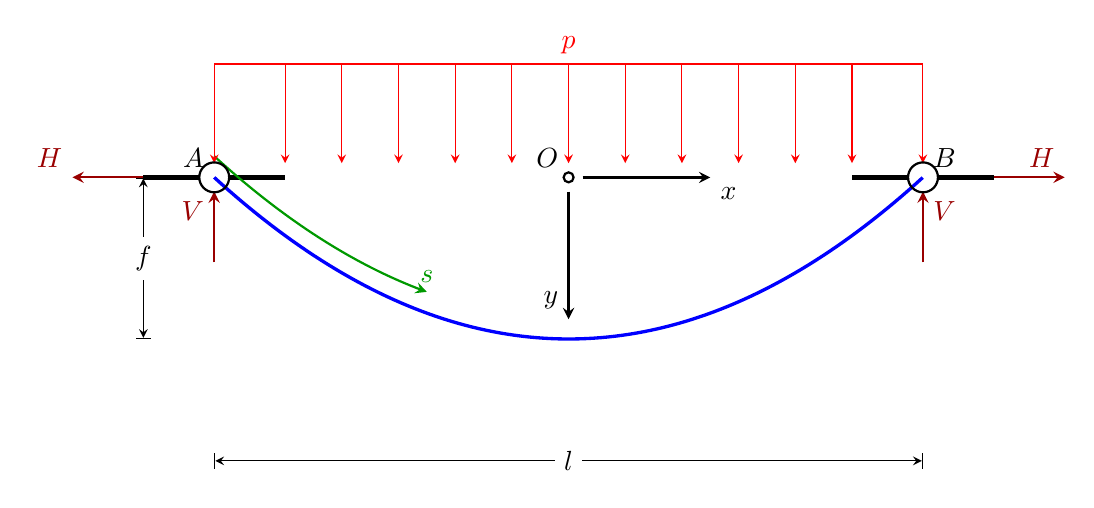
\begin{tikzpicture}[scale=1.8, >=stealth]
% Stile per i vincoli (muro/soffitto)
\tikzset{ground/.style={fill,pattern=north east lines,draw=none,minimum width=0.75cm,minimum height=0.3cm}}

% Parametri geometrici della parabola per il plot matematico
\def\l{5}   % Luce (lunghezza totale)
\def\f{1.14} % Freccia (distanza verticale dal vertice ad A/B: 3 - 1.86 = 1.14)

% Coordinate dei supporti
\coordinate (A) at (0,3);
\coordinate (B) at (5,3);
\coordinate (HA) at (-0.5,3);
\coordinate (HB) at (5.5,3);
\coordinate (VA) at (0,2.4);
\coordinate (VB) at (5,2.4);
\coordinate (O) at (2.5, 3);

% Rappresentazione dei supporti fisici
\draw[ultra thick] (-0.5,3) -- (-0.1,3);
\draw[ultra thick] ( 0.1,3) -- (0.5,3);
\draw[ultra thick] (4.5,3)  -- (4.9,3);
\draw[ultra thick] (5.1,3)  -- (5.5,3);

% --- LA FUNE (PARABOLA REALE) ---
% Equazione: y = 3 - f * (1 - (2*x/l - 1)^2)
\draw[very thick, blue, samples=100, domain=0:\l] 
    plot (\x, {3 - \f*(1 - (2*\x/\l-1)^2)});

% --- TRATTO DI ASCISSA CURVILINEA s (PARALLELA ALLA PARABOLA) ---
% Parte da A (x=0) e arriva fino a x=1.5, con un offset verticale di -0.15 per parallelismo
\draw[->, green!60!black, thick, samples=50, domain=0:1.5] 
    plot (\x, {3 - \f*(1 - (2*\x/\l-1)^2) + 0.15});

% Tratteggio verticale che collega la fine di 's' alla fune blue
\coordinate (S_end) at (1.5, {3 - \f*(1 - (2*1.5/\l-1)^2) + 0.15});
\coordinate (Fune_match) at (1.5, {3 - \f*(1 - (2*1.5/\l-1)^2)});

% Posizionamento MANUALE e preciso della lettera 's' sotto la punta della freccia verde
    \node[green!60!black, above] at (S_end) {$s$};

% --- CARICO DISTRIBUITO RETTANGOLARE SOPRA LA RETTA AB ---
\begin{scope}[shift={(A)}]
    \def\lung{5}      
    \def\alt{0.8}     
    
    \draw[red] (0, 0.1) -- (0, \alt) -- (\lung, \alt) -- (\lung, 0.1);
    
    \foreach \x in {0, 0.5, 0.9, 1.3, 1.7, 2.1, 2.5, 2.9, 3.3, 3.7, 4.1, 4.5, 5} {
        \draw[->, red, ] (\x, \alt) -- (\x, 0.1);
        }
    
    \node[red, above] at ({\lung/2}, \alt) {$p$};
\end{scope}

% --- QUOTE ---
\draw[black, thin, |<->|] (0, 1) -- (5, 1) node[midway, fill=white] {$l$};
\draw[black, thin, |<->|] (-0.5, 3) -- (-0.5, 1.86) node[midway, fill=white] {$f$};

% --- SISTEMA DI RIFERIMENTO ---
\draw[thick] (O) circle (1pt) node[above left] {$O$};
\draw[->, black, thick] (2.6, 3 ) -- (3.5, 3) node[below right]{${x}$};
\draw[->, black, thick] (2.5, 2.9 ) -- (2.5, 2) node[above left]{${y}$};

% Tensioni agli estremi
\draw[->, red!60!black, thick] (VA) -- ++( 0.0, 0.5) node[below left] {${V}$};
\draw[->, red!60!black, thick] (VB) -- ++( 0.0, 0.5) node[below right] {${V}$};
\draw[->, red!60!black, thick] (HA) -- ++(-0.5, 0.0) node[above left] {${H}$};
\draw[->, red!60!black, thick] (HB) -- ++( 0.5, 0.0) node[above left] {${H}$};

% Nodi di testo per i punti
\draw[thick] (A) circle (3pt) node[above left] {$A$};
\draw[thick] (B) circle (3pt) node[above right] {$B$};

\end{tikzpicture}
    \caption{Fune soggetta ad un carico verticale distribuito uniforme}
    \label{fig:fune_carico_distr}
\end{figure}
L'equilibrio di un tratto di fune compreso tra l'estremo $A$ ed una sezione generica di ascissa $x$ porta alla relazione: 

\begin{equation}
   H y(x) -  \frac{pl}{2}\left( \frac{l}{2} + x \right) + \frac{p}{2}\left( \frac{l}{2} + x \right)^{2} = 0
\end{equation}

Scrivendo la relazione in modo da esplicitare $y(x)$, avremo: 

\begin{equation}
   y(x) = \frac{p}{2H} \left( \frac{l^{2}}{4} - x^{2} \right) 
\end{equation}

La fune assume quindi la forma di una parabola simmetrica rispetto all'asse verticale. 
La tiro orizzontale risulta quindi:
\begin{equation}
   H = \frac{pl^{2}}{8f}
   \label{eq:equazione_tiro}
\end{equation}
Conoscendo $p$, $l$ ed $f$, e quindi la geometria della configurazione deformata, è immediato ricavare il tiro orizzontale $H$. Di conseguenza, la formula permette di conoscere il tiro di una fune già installata, quando la freccia $f$ può essere misurata, ma non consente di determinare a priori il tiro necessario per ottenere una configurazione desiderata. 

\subsubsection{L'equilibrio della fune soggetta al peso proprio}
Consideriamo la configurazione deformata di una fune soggetta al peso proprio.

\begin{figure}[htbp]
    \centering
    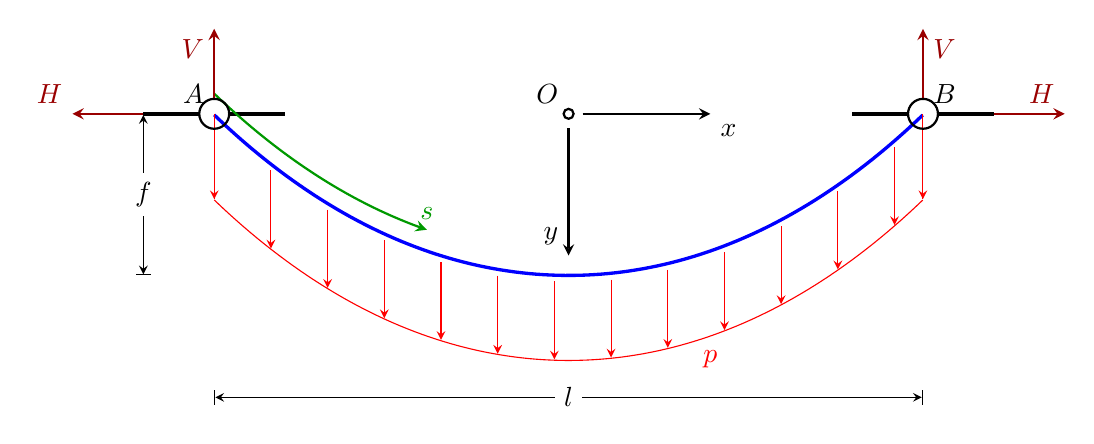
\begin{tikzpicture}[scale=1.8, >=stealth]
% Stile per i vincoli (muro/soffitto)
\tikzset{ground/.style={fill,pattern=north east lines,draw=none,minimum width=0.75cm,minimum height=0.3cm}}

% Parametri geometrici della catenaria per il plot matematico
\def\l{5}       % Luce (lunghezza totale)
\def\f{1.14}    % Freccia
\def\a{2.93}    % Parametro della catenaria per avere f=1.14 con l=5
\def\yv{1.86}   % Quota del vertice in mezzeria (3 - 1.14)

% Coordinate dei supporti
\coordinate (A) at (0,3);
\coordinate (B) at (5,3);
\coordinate (HA) at (-0.5,3);
\coordinate (HB) at (5.5,3);
\coordinate (VA) at (0,3.1);
\coordinate (VB) at (5,3.1);
\coordinate (O) at (2.5, 3);

% Rappresentazione dei supporti fisici
\draw[ultra thick] (-0.5,3) -- (-0.1,3);
\draw[ultra thick] ( 0.1,3) -- (0.5,3);
\draw[ultra thick] (4.5,3)  -- (4.9,3);
\draw[ultra thick] (5.1,3)  -- (5.5,3);

% --- LA FUNE (CATENARIA REALE) ---
% Equazione: y = yv + a * (cosh((x-2.5)/a) - 1) espressa in forma esponenziale
\draw[very thick, blue, samples=100, domain=0:\l] 
    plot (\x, {\yv + \a*(0.5*(exp((\x-2.5)/\a) + exp(-(\x-2.5)/\a)) - 1)});

% --- TRATTO DI ASCISSA CURVILINEA s (PARALLELA ALLA CATENARIA) ---
\draw[->, green!60!black, thick, samples=50, domain=0:1.5] 
    plot (\x, {\yv + \a*(0.5*(exp((\x-2.5)/\a) + exp(-(\x-2.5)/\a)) - 1) + 0.15});

% Posizionamento della lettera 's' sopra la punta della freccia verde
\pgfmathsetmacro{\xS}{1.5}
\pgfmathsetmacro{\yS}{\yv + \a*(0.5*(exp((\xS-2.5)/\a) + exp(-(\xS-2.5)/\a)) - 1) + 0.15}
\node[green!60!black, above] at (\xS,\yS) {$s$};

% --- CARICO DISTRIBUITO LUNGO LA FUNE (PESO PROPRIO) ---
% Profilo superiore del carico (offset di +0.6 verticalmente rispetto alla catenaria)
\draw[red, thin] plot[samples=100, domain=0:\l] 
    (\x, {\yv + \a*(0.5*(exp((\x-2.5)/\a) + exp(-(\x-2.5)/\a)) - 1) - 0.6});

% Chiusure laterali del diagramma di carico agli appoggi
\draw[red, thin] (0,3) -- (0,2.4);
\draw[red, thin] (5,3) -- (5,2.4);

% Generazione delle frecce di carico verticali che seguono l'andamento della fune
\foreach \x in {0, 0.4, 0.8, 1.2, 1.6, 2.0, 2.4, 2.8, 3.2, 3.6, 4.0, 4.4, 4.8, 5.0} {
    \pgfmathsetmacro{\yline}{\yv + \a*(0.5*(exp((\x-2.5)/\a) + exp(-(\x-2.5)/\a)) - 1.22)}
    \draw[->, red, thin] (\x, {\yline + 0.6}) -- (\x, {\yline + 0.05});
}
% Etichetta del carico costante lungo la curva
\node[red, below] at (3.5, 1.4) {$p$};

% --- QUOTE ---
\draw[black, thin, |<->|] (0, 1) -- (5, 1) node[midway, fill=white] {$l$};
\draw[black, thin, |<->|] (-0.5, 3) -- (-0.5, 1.86) node[midway, fill=white] {$f$};

% --- SISTEMA DI RIFERIMENTO ---
\draw[thick] (O) circle (1pt) node[above left] {$O$};
\draw[->, black, thick] (2.6, 3 ) -- (3.5, 3) node[below right]{${x}$};
\draw[->, black, thick] (2.5, 2.9 ) -- (2.5, 2) node[above left]{${y}$};

% Tensioni agli estremi
\draw[->, red!60!black, thick] (VA) -- ++( 0.0, 0.5) node[below left] {${V}$};
\draw[->, red!60!black, thick] (VB) -- ++( 0.0, 0.5) node[below right] {${V}$};
\draw[->, red!60!black, thick] (HA) -- ++(-0.5, 0.0) node[above left] {${H}$};
\draw[->, red!60!black, thick] (HB) -- ++( 0.5, 0.0) node[above left] {${H}$};

% Nodi di testo per i punti
\draw[thick] (A) circle (3pt) node[above left] {$A$};
\draw[thick] (B) circle (3pt) node[above right] {$B$};

\end{tikzpicture}
    \caption{Fune soggetta al peso proprio.}
    \label{fig:fune_catenaria}
\end{figure}
Sia $\gamma$ il peso specifico lineare della fune. L'equilibrio di un tratto compreso tra le ascisse curvilinee $s_1$ e $s_2$ fornisce: 

\begin{equation}
   V(s_2)-V(s_1) + \gamma(s_2 - s_1) = 0
\end{equation}
Passando al limite per $s_2 \rightarrow s_1$ si ottiene l'equazione indefinita di equilibrio: 

\begin{equation}
   \frac{dV}{ds} + \gamma = 0 
   \label{eq:indefinita_equilibrio}
\end{equation}
Poichè lo sforzo normale è parallelo alla tangente alla fune, vale la relazione: 
\begin{equation}
   V(s) = H\frac{dy}{dx}
   \label{eq:parallelismo}
\end{equation}
Inoltre, la lunghezza infinitesima della configurazione deformata $ds$ è: 
\begin{equation}
  ds = \sqrt{1 + (y'(x))^{2}} dx
  \label{eq:ds}
\end{equation}
Sostituendo le espressioni \eqref{eq:parallelismo} e \eqref{eq:ds} nella \eqref{eq:indefinita_equilibrio}, si ottiene:
\begin{equation}
   \frac{d^{2}y}{dx^{2}} = - \frac{\gamma}{H} \sqrt{1 + \left( \frac{dy}{dx} \right)^{2}}
\end{equation} 
che rappresenta l'equazione differenziale della catenaria. 
Risolvendo, troviamo l'equazione generale della catenaria:
\begin{equation}
   y(x) = - \frac{H}{\gamma}cosh \left[ \frac{\gamma}{H} (x - x_0)\right] + y_0
   \label{eq:equazione_generale_della_catenaria}
\end{equation}
dove $x_0$ e $y_0$ sono costanti di integrazione. Imponendo le condizioni al bordo coerentemente con \cref{fig:fune_catenaria} otteniamo la soluzione particolare del problema della catenaria:
\begin{equation}
   y(x) = \frac{H}{\gamma} \left( \cosh\!\left(\frac{\gamma l}{2H}\right) - \cosh\!\left(\frac{\gamma x}{H}\right) \right)
   \label{eq:equazione_particolare_della_catenaria}
\end{equation}

\subsubsection{La fune soggetta ad un accorciamento iniziale}
Nel modello inestensibile, la lunghezza della fune nella configurazione deformata coincide necessariamente con la lunghezza iniziale $L_0$. Tuttavia, nella pratica ingegneristica si presentano frequentemente situazioni in cui la fune viene installata con una lunghezza differente rispetto a quella che assumerebbe in assenza di carico, ad esempio a causa di un accorciamento $\Delta L_0$ imposto in fase di montaggio. 
Per modellare tali condizioni, si introduce una \textbf{lunghezza efficace} della fune, definita come: 
\begin{equation}
    L_{eff} = L_0 - \Delta L_0 = L_0(1 - \varepsilon_0) 
    \label{eq:lunghezza_efficace}
\end{equation}
dove $\varepsilon_0$ non rappresenta una deformazione imposta al materiale, ma è la percentuale di lunghezza iniziale del cavo che produce l'accorciamento desiderato. L'idea è quella di considerare la fune come inestensibile, ma con una lunghezza iniziale modificata. 

\subsubsection{L'equazione di congruenza}
Nei modelli inestensibili analizzati, l'equilibrio fornisce la forma della fune in funzione del tiro orizzontale $H$. Tuttavia, né nel caso della parabola né in quello della catenaria la geometria deformata è nota a priori: essa dipende proprio dal valore di $H$.
Quando, oltre ai carichi esterni $p$ (o $\gamma$) e alla distanza tra gli appoggi $l$, è nota anche la lunghezza iniziale della fune $L_0$, è possibile chiudere il problema imponendo una condizione di congruenza sulla lunghezza.
Per una fune inestensibile, la lunghezza nella configurazione deformata deve coincidere con la lunghezza iniziale. L'ipotesi costitutiva si traduce quindi nella condizione:
\begin{equation}
   L = L_0
   \label{eq:congruenza_inestensibile}
\end{equation}
La lunghezza $L$ dipende dalla forma della fune e quindi dal tiro $H$. In entrambe i problemi vale la seguente relazione: 
\begin{equation}
 L(H) = \int_{0}^{L} ds\ = \int_{-\frac{l}{2}}^{\frac{l}{2}} \sqrt{1 + (y'(x; H))^{2}} dx\
 \label{eq:lunghezza_deformata}
\end{equation}
Imporre la congruenza significa quindi risolvere l'equazione non lineare: 
\begin{equation}
   L(H) - L_0 = 0
   \label{eq:congruenza_inestensibile2}
\end{equation}
che combina equilibrio e congruenza e permette di determinare il tiro orizzontale $H$. 
Nel caso in cui la fune sia soggetta ad un accorciamento iniziale, la lunghezza disponibile dopo l'operazione non coincide più con $L_0$, ma con la lunghezza efficace $L_{eff}$. L'equazione di congruenza diventa: 
\begin{equation}
   L(H) = L_{eff}
   \label{eq:congruenza_inestensibile_con accorciamento}
\end{equation}
Ed il problema non lineare da risolvere assume la forma:
\begin{equation}
   L(H) - L_{eff} = 0
   \label{eq:congruenza_inestensibile2_con_accorciamento}
\end{equation}
Poichè per l'ipotesi di inestensibilità della fune dovrà valere che: 
\begin{equation}
   L(H) = L_{eff} \geq l
   \label{eq:condizione_di_esistenza_della_soluzione}
\end{equation}
L'equazione di congruenza ammette soluzione solo se la lunghezza efficace non è inferiore alla distanza tra gli appoggi. Di fatto nessuna fune inestensibile può assumere una configurazione con lunghezza inferiore alla distanza tra i vincoli. 

\vspace{1em}
Nelle figura \cref{fig:parabolavscatenaria} vengono presentati i grafici delle deformate di una fune inestensibile ($l = 10m$) soggetta al peso proprio, analizzata secondo i due principali schemi di carico verticale: distribuito sullo sviluppo della fune oppure sulla distanza orizzontale tra gli appoggi. Il confronto evidenzia come la differenza tra i due approcci sia marcata nel caso di funi lasche ($L_{eff} > l$) mentre diventi trascurabile nel casi di funi tese ($L_{eff} \approx l$), come mostrato nella figura \cref{fig:parabolavscatenaria2}, attraverso il grafico degli scostamenti geometrici.

\begin{figure}[htbp]
    \centering
    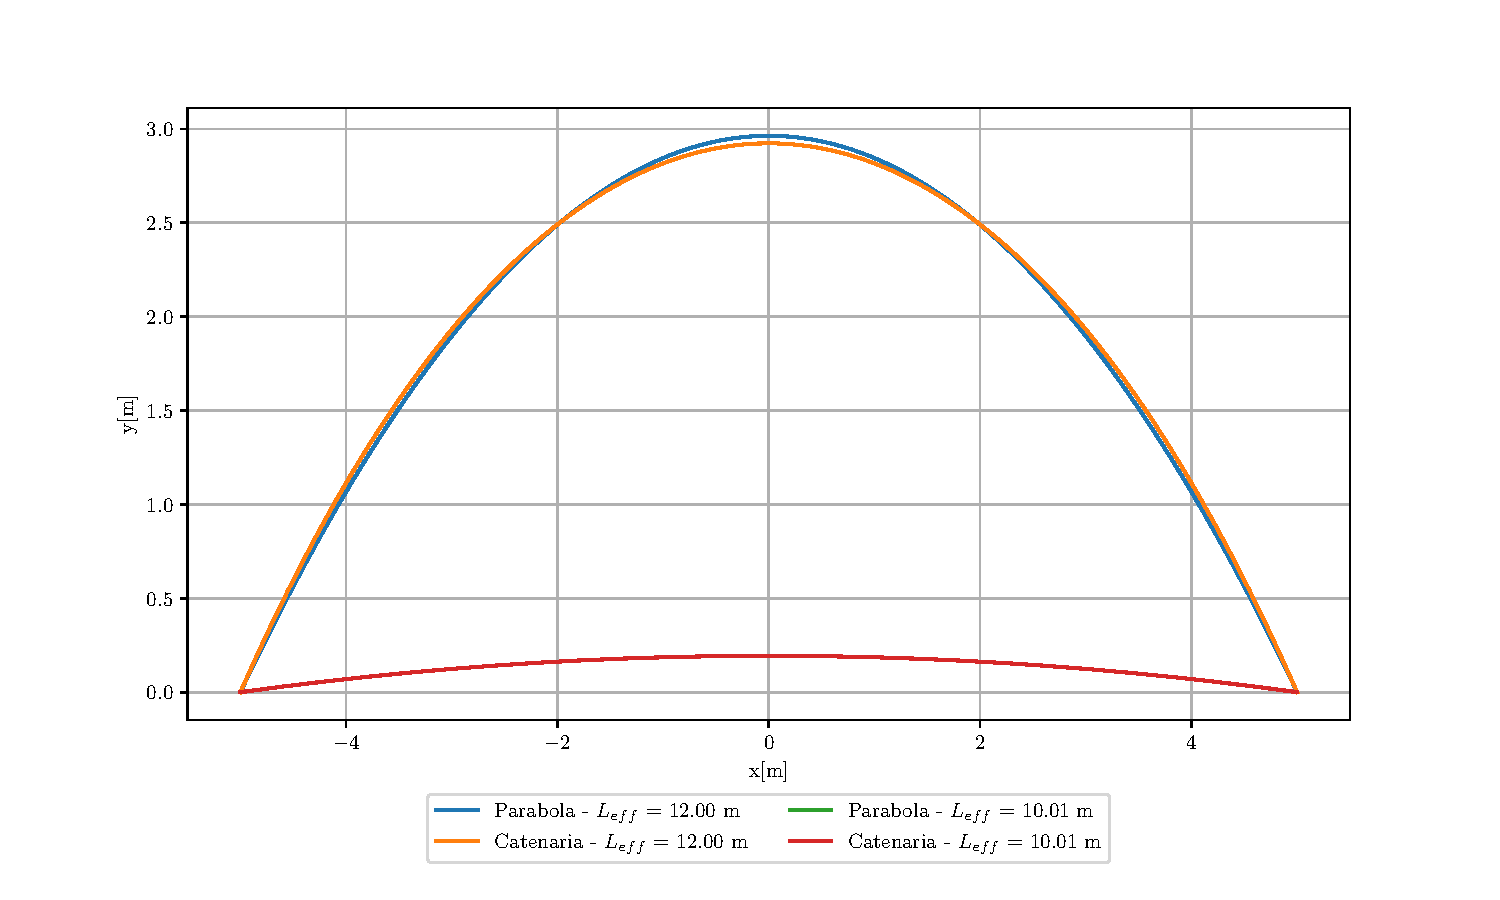
\includegraphics[width=\textwidth]{143_capitoli/capitolo2/immagini_capitolo_2/parabolavscatenaria.pdf}
    \caption{Deformata della fune: modello parabolico vs catenaria}
    \label{fig:parabolavscatenaria}
\end{figure}

\begin{figure}[htbp]
    \centering
    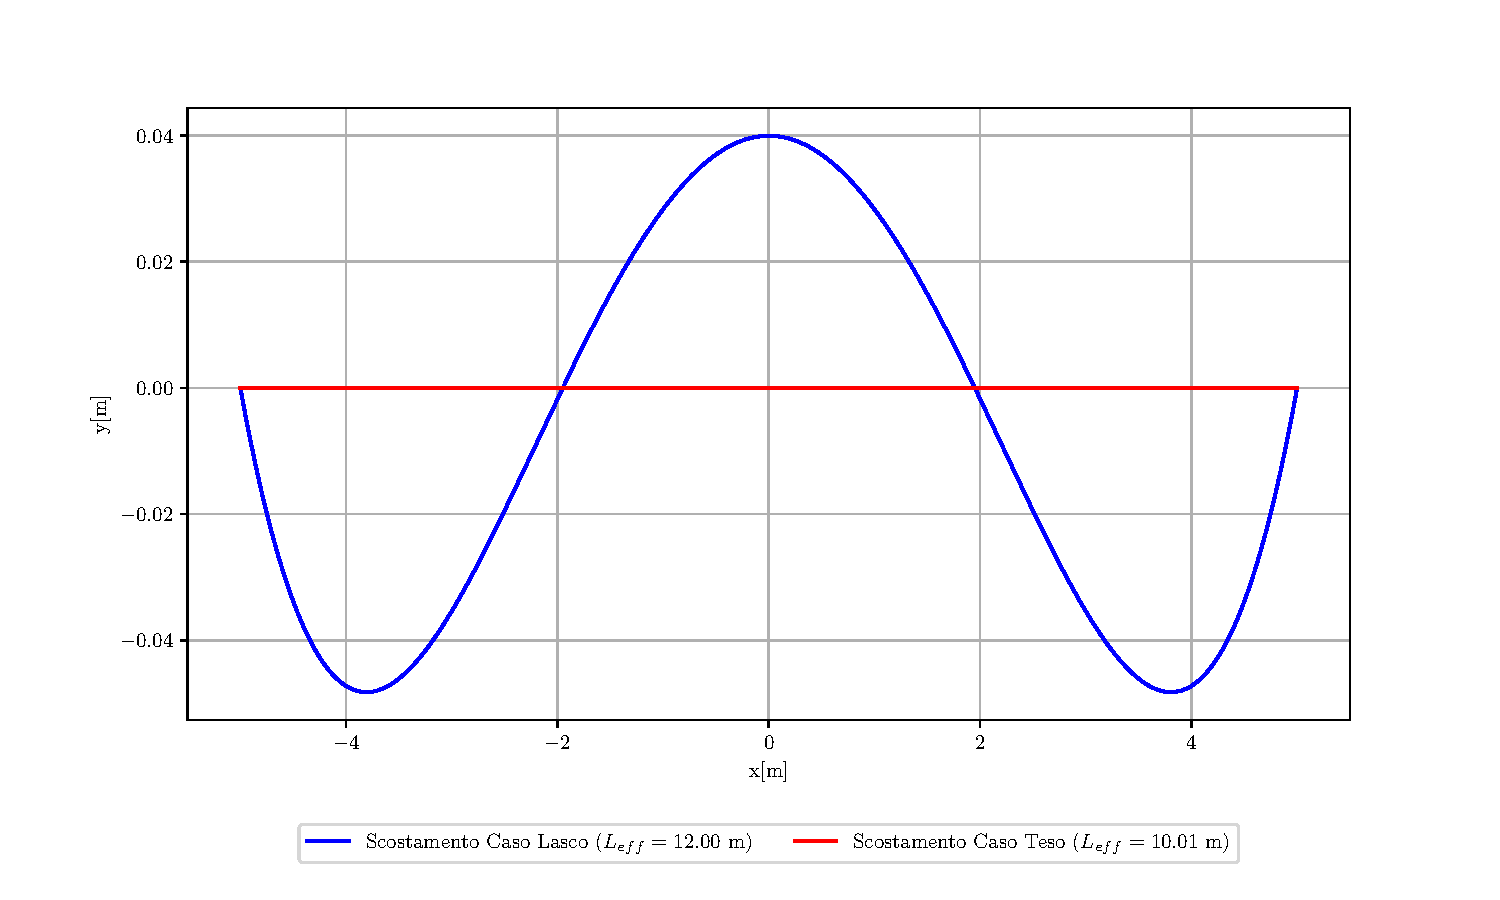
\includegraphics[width=\textwidth]{143_capitoli/capitolo2/immagini_capitolo_2/parabolavscatenaria2.pdf}
    \caption{Scostamento geometrico locale: modello parabolico vs catenaria}
    \label{fig:parabolavscatenaria2}
\end{figure}

\vspace{1em}
Il modello di fune inestensibile rappresenta uno strumento teorico estremamente efficace per descrivere in modo semplice e diretto la meccanica delle funi. La possibilità di ricavare le soluzioni per la parabola e per la catenaria, ne fanno un punto di partenza per i modelli successivi. Tuttavia, la sua semplicità deriva da assunzioni che ne limitano significativamente il campo di applicazione. In particolare, il modello non consente di rappresentare: 
\begin{itemize}
   \item la deformazione assiale del cavo. 
   \item il problema delle funi con lunghezza iniziale inferiore alla distanza tra gli appoggi. 
   \item il problema della fune con accorciamento della lunghezza iniziale tale per cui $L_{eff}<l$
\end{itemize}
La fune inestensibile è un modello geometrico, non costitutivo, utile per descrivere la forma in equilibrio ma incapace di rappresentare l'evoluzione deformativa o gli effetti della deformabilità assiale. 
Per affrontare il problema anche dal punto di vista deformativo e costitutivo è indispensabile ricorrere a modelli più completi, come il modello di Irvine, soluzioni numeriche al problema elastico non lineare o le formulazioni numeriche alle differenze finite o agli elementi finiti. 

\subsection{La fune elastica}
Il modello analizzato in questa sezione introduce un legame costitutivo esplicito tra spostamenti, deformazioni e tensioni. Questo approccio permette di superare le limitazioni intrinseche del modello inestensibile, le quali risultano fortemente vincolanti nella pratica progettuale (come l'impossibilità di modellare funi con lunghezza efficace inferiore alla distanza tra gli appoggi).

Inizialmente verrà introdotto il legame costitutivo del cavo; successivamente, verrà formulata l'equazione di congruenza che tiene conto dell'allungamnto assiale, al fine di determinare il tiro orizzontale $H$ attraverso una strategia numerica.

\vspace{1em}
Introduciamo il legame costitutivo  elastico lineare per il materiale: 
\begin{equation}
   \varepsilon = \frac{\sigma}{E}
   \label{eq:legame_costitutivo_materiale}
\end{equation}
Il quale, espresso in termini di sforzo normale $N$  e rigidezza assiale del cavo $EA$ assume la forma: 
\begin{equation}
   \varepsilon = \frac{N}{EA}
   \label{eq:legame_costitutivo_cavo}
\end{equation}
Coerentemente con le figure \cref{fig:fune_catenaria} e \cref{fig:fune_carico_distr}, difiniamo $s_0$ ed $s$, rispettivamente, l'ascissa curvilinea della fune nella configurazione iniziale e finale. 
Assumendo l'ipotesi di piccole deformazioni elastiche del materiale, la deformazione assiale può essere espressa mediante la relazione cinematica classica:
\begin{equation}
   \varepsilon = \frac{ds - ds_0}{ds_0}
   \label{eq:deformazione_assiale}
\end{equation}
dove $ds_0$ e $ds$ sono rispettivamente il tratto infinitesimo dell'ascissa curvilinea nelle due configurazioni.
Combinando la relazione \eqref{eq:deformazione_assiale} con il legame costitutivo \eqref{eq:legame_costitutivo_cavo}, è possibile esplicitare il tratto differenziale iniziale $ds_0$ in funzione della geometria deformata corrente e dello sforzo agente: 
\begin{equation}
   ds_0 = \frac{EA}{EA + N(s)} ds
   \label{eq:ds0_funzione_ds}
\end{equation}
L'equazione \eqref{eq:ds0_funzione_ds} consente di mappare la lunghezza iniziale della fune a partire dalla configurazione finale di equilibrio.

Per stabilire la condizione di congruenza del problema elastico, si consideri la lunghezza totale della fune nella configurazione finale deformata $L(H)$. Essa sarà pari alla lunghezza iniziale $L_0$ maggiorata dell'allungamento totale elastico $\Delta L$ indotto dai carichi:
\begin{equation}
   L(H) - \Delta L - L_0 = 0
   \label{eq:congruenza_estensibile}
\end{equation}
Ipotizziamo nota la lunghezza del cavo in configurazione iniziale $L_0$, l'equazione di congruenza \eqref{eq:congruenza_estensibile} può essere riscritta isolando la quantità geometrica iniziale:
\begin{equation}
   L(H) - \Delta L  = L_0
   \label{eq:congruenza_estensibile2}
\end{equation}
Ricordando che lo sforzo normale lungo il profilo della fune è legato al tiro orizzontale $H$ dalla relazione:
\begin{equation}
   N(x) = H \sqrt{1 + (y'(x; H))^2}
   \label{eq:sforzo_normale}
\end{equation}
e che il differenziale corrente $ds$ sulla corda è espresso mediante la relazione \eqref{eq:ds}, la lunghezza iniziale $L_0$ può essere calcolata integrando l'equazione \eqref{eq:ds0_funzione_ds} lungo la proiezione orizzontale della campata $l$:
\begin{equation}
    L_0(H) = \int_{0}^{L_0} ds_0\ = \int_{-\frac{l}{2}}^{\frac{l}{2}} \frac{EA}{EA + N(x)} \sqrt{1 + (y'(x; H))^{2}} dx\
   \label{eq:lunghezza_indeformata_integer}
\end{equation}
Il problema di congruenza si riduce pertanto alla risoluzione di un equazione non lineare nella sola incongnita rappresentata dal tiro orizzontale $H$: 
\begin{equation}
   L_0 - L_0(H) = 0 
   \label{eq:residuo_congruenza}
\end{equation}
Poichè la funzione della lunghezza elastica $L_0(H)$ dipende in modo fortemente non lineare da $H$, l'equazione \eqref{eq:residuo_congruenza} non ammette una soluzione analitica in forma chiusa. Il problema può essere tuttavia risolto efficacemente mediante schemi iterativi numerici, come il metodo di Newton - Raphson.

\vspace{1em}
Consideriamo anche in questo caso la necessità, dato un cavo di lunghezza inizale $L_0$, di sottoporlo ad un accorciamento $\Delta L_0$. Tale condizione modella fenomeni fisici reali importanti nell'ingegneria, come le operazioni di pre-tensionamento meccanico agli ancoraggi, i difetti di montaggio in cantiere e le contrazioni termiche indotte. Coerentemente con quanto definito per il modello inestensibile, si introduce la \textbf{lunghezza efficace} della fune in configurazione indeformata, definita come:
\begin{equation}
    L_{eff} = L_0 - \Delta L_0 = L_0(1 - \varepsilon_0)
    \label{eq:lunghezza_efficace_elastica}
\end{equation}
dove $\varepsilon_0$ rappresenta l'aliquota di accorciamento percentuale impresso rispetto alla geometria iniziale. L'introduzione di $L_{eff}$ modifica l'equazione di congruenza. La fune vincolata agli appoggi distanti $l$, reagisce alla contrazione sviluppando uno stato di trazione interna, nel caso in cui $L_{eff}<l$, mentre produce una variazione geometrica pari a quella prodotta nel caso inestensibile, quando $L_{eff}>l$. Al fine di esplicitare il ruolo di ciascuna componente deformativa la lunghezza totale della fune nella configurazione deformata $L$ può essere vista come la somma algebrica della lunghezza efficace $L_{eff}$, dell'accorciamento di montaggio $\Delta L_0$ e dell'allungamento elastico $\Delta L$:
\begin{equation}
   L = L_{eff} + \Delta L_0 + \Delta L
   \label{eq:contributi_L}
\end{equation}
Ricordando che per definizione l'allungemento elastico totale è pari a: 
\begin{equation}
   \Delta L = L - L_0(H)
   \label{eq:delta_L}
\end{equation}
la relazione di congruenza \eqref{eq:contributi_L} si riduce immediatamente all'uguaglianza:
\begin{equation}
L_0(H) = L_{eff} + \Delta L_0 \implies L_0(H) = L_0
\end{equation}
Il problema si riduce nuovamente alla determinazione dello zero di una funzione nella sola incognita $H$, pronta per essere implementata nell'algoritmo di Newton-Raphson.

\vspace{1em}
Prendiamo ad esempio una fune in acciaio (possiamo assumere che il modulo elastico sia pari a $E = 210GPa$ e che la densità valga $7850kg/m$), di area pari ad $A = \pi r^{2}$ con $r = 1cm$, soggetta all'azione del solo peso proprio lineare ($\gamma = \rho g A$) considerata agente sulla lunghezza della fune stessa, la cui distanza tra gli appoggi è pari a $l$. Ipotizzando di conoscere la lunghezza iniziale $L_0$ e variando la $L_{eff}$ per mezzo di un accorciamento $\Delta L$, grazie alle figure \cref{fig:estensibilevsinestensibile1} e \cref{fig:estensibilevsinestensibile2} possiamo vedere come attraverso il modello estensibile si possano considerare anche problemi la cui $L_{eff}$ sia minore di $l$. Nella figura \cref{fig:estensibilevsinestensibile3}, in cui si mette in relazione il tiro $H$ con la lunghezza effettiva della fune $L_{eff}$ il limite del modello inestensibile viene fuori. Osserviamo come il comportamento ottenuto dal modello estensibile quando la lunghezza $L_{eff}$ è inferiore alla luce $l$ assume un comportamento lineare proporzionale alla rigidezza assiale $EA$ della fune, mentre nel modello inestensibile, per $L_{eff} \approx l$ la curva incontra un asintoto verticale. Naturalmente il modello estensibile ci permette di cogliere anche il comportamento limite della fune la cui rigidezza assiale sia rispetto ai carichi esterni considerabile come inestensibile, di fatti per $EA \rightarrow \infty $, la curva del modello estensibile tenderà a quella del modello inestensibile.

\begin{figure}[H]
    \centering
    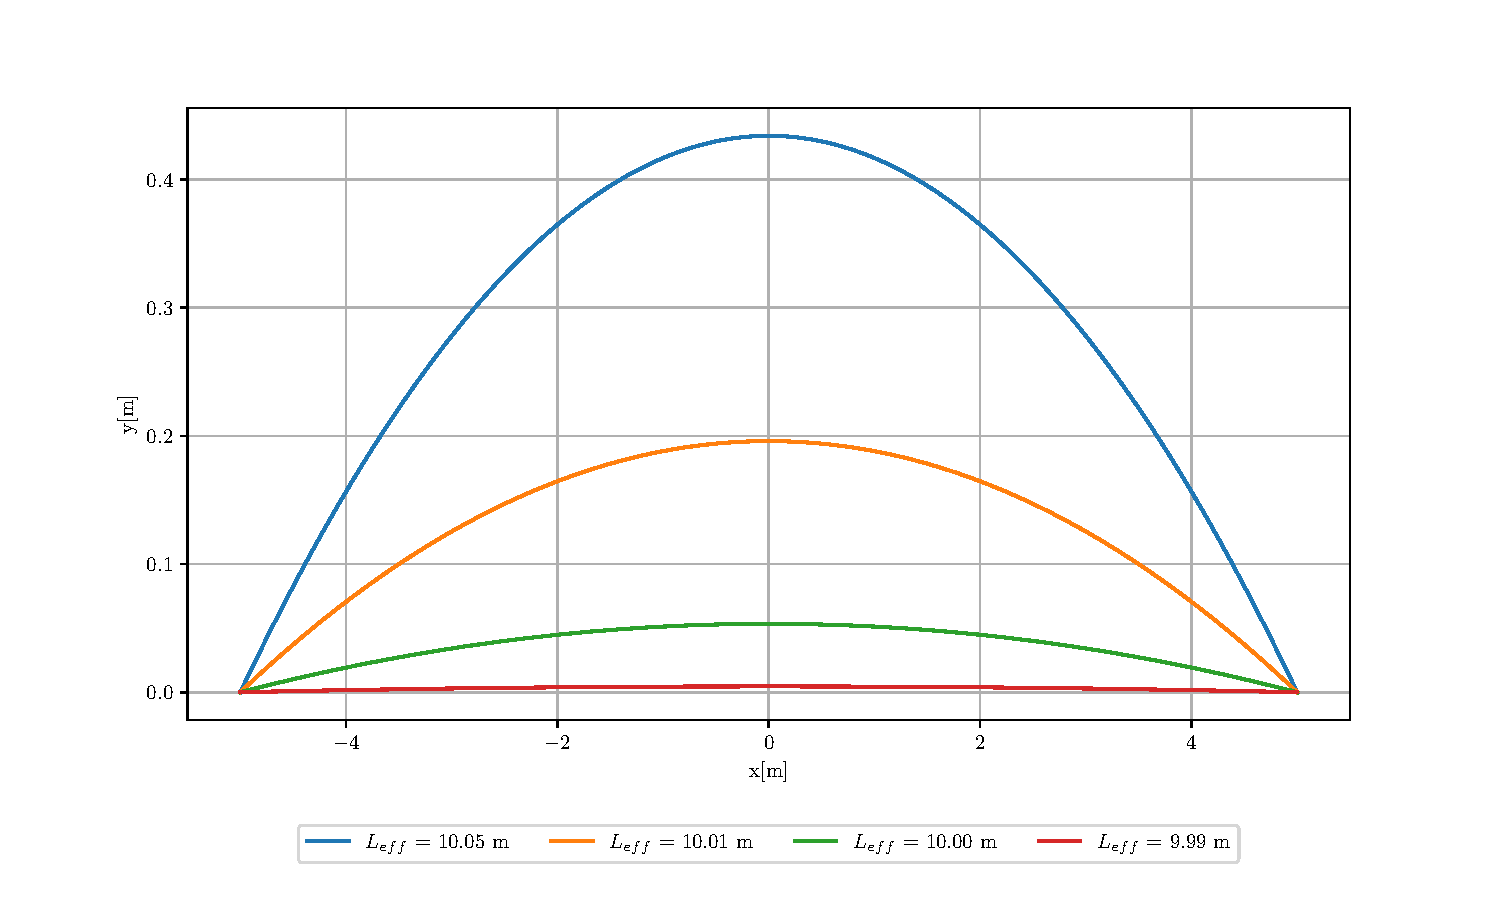
\includegraphics[width=\textwidth]{143_capitoli/capitolo2/immagini_capitolo_2/estensibilevsinestensibile1.pdf}
    \caption{Deformata della fune per varie $L_{eff}$}
    \label{fig:estensibilevsinestensibile1}
\end{figure}

\begin{figure}[H]
    \centering
    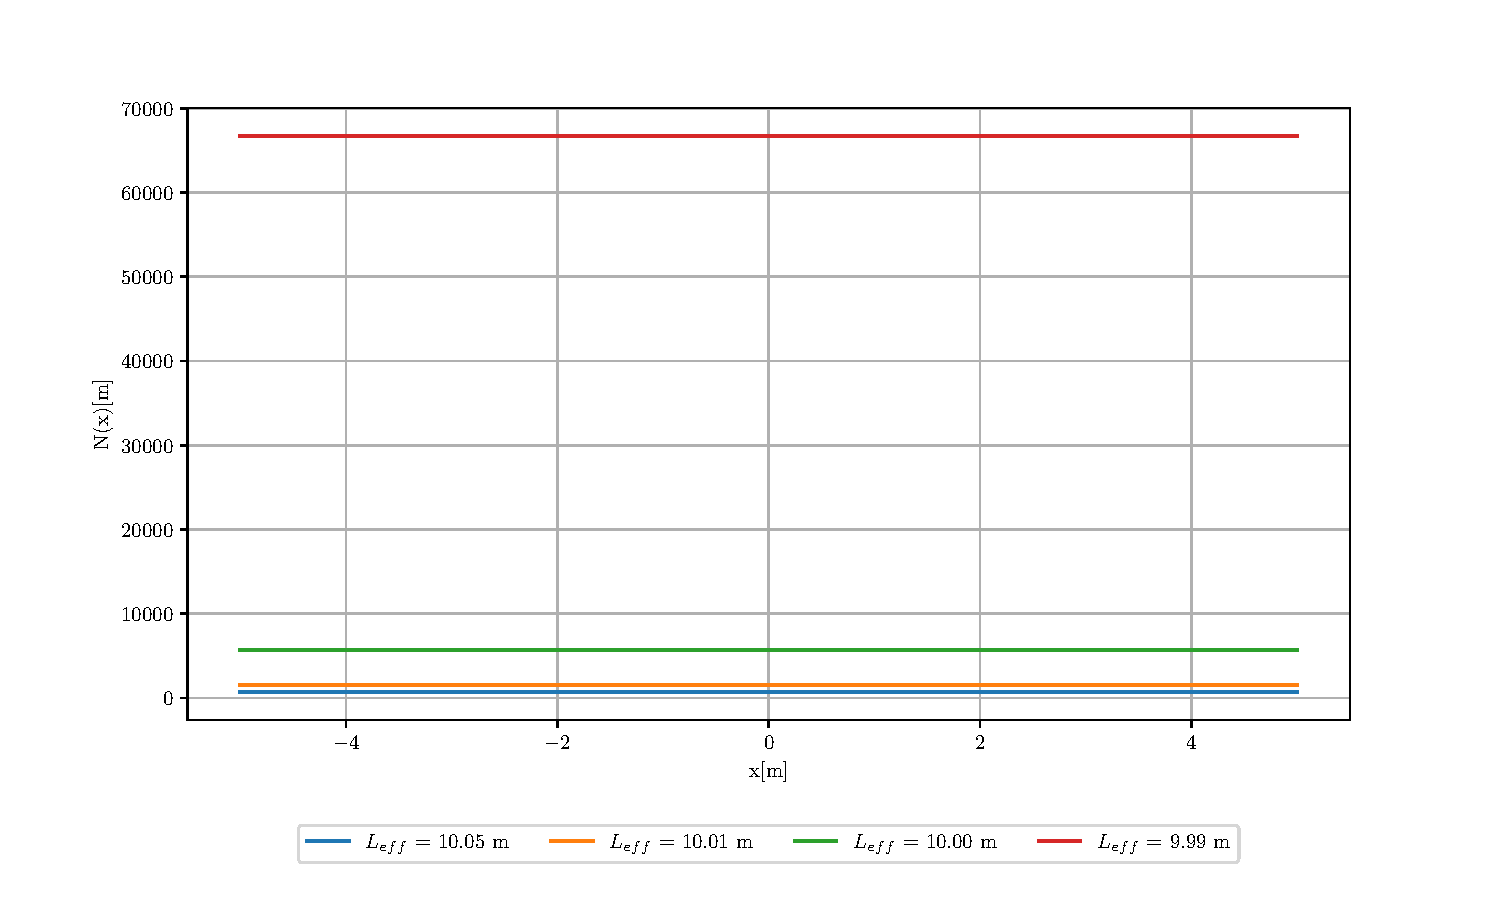
\includegraphics[width=\textwidth]{143_capitoli/capitolo2/immagini_capitolo_2/estensibilevsinestensibile2.pdf}
    \caption{Sforzo normale nella fune per varie $L_{eff}$}
    \label{fig:estensibilevsinestensibile2}
\end{figure}

\begin{figure}[H]
    \centering
    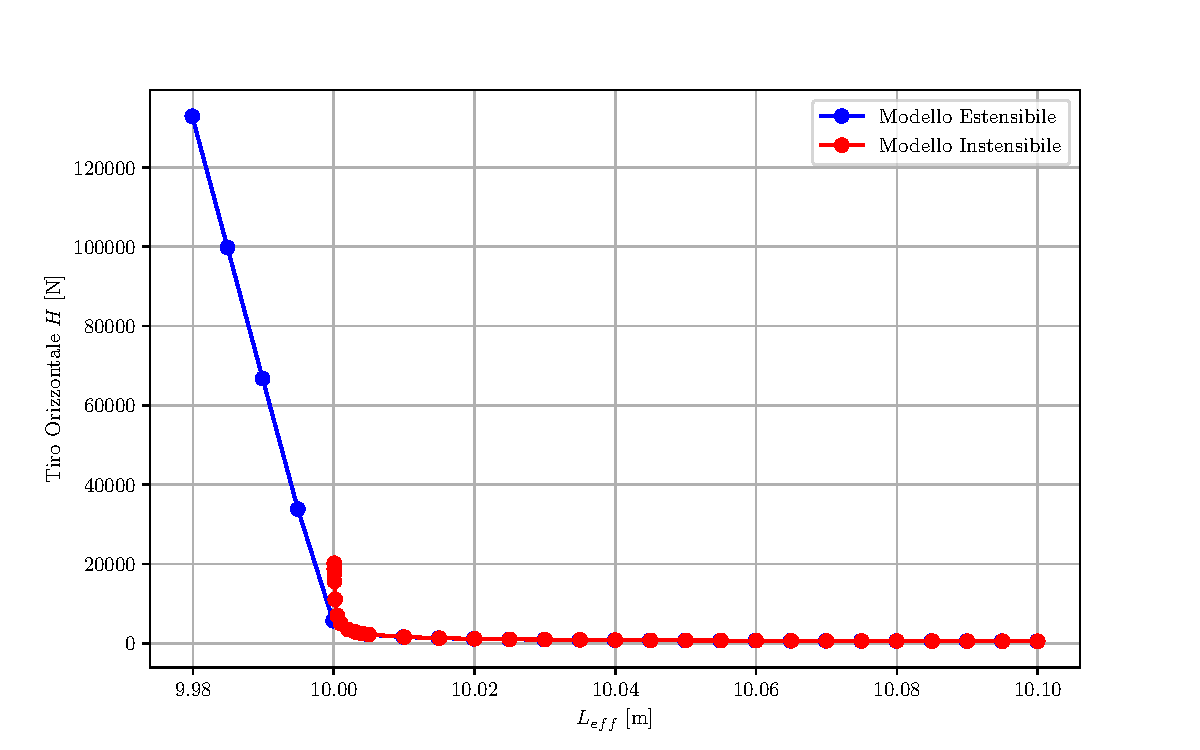
\includegraphics[width=\textwidth]{143_capitoli/capitolo2/immagini_capitolo_2/estensibilevsinestensibile3.pdf}
    \caption{Curva $L_{eff}$ - $H$: modello estensibile vs inestensibile}
    \label{fig:estensibilevsinestensibile3}
\end{figure}

\vspace{1em}
\subsection{Una soluzione alle differenze finite}
Mentre i modelli basati sull'equazione globale di congruenza della catenaria elastica introducono limitazioni cinematiche e matematiche, lo schema numerico che proponiamo mira alla risoluzione diretta della formulazione differenziale indefinita di Irvine. Tale approccio, in accordo con quanto riportato in \cite{irvine1981}, offre tre vantaggi fondamentali: in primo luogo, tratta la geometria corrente come incognita pura; in secondo luogo, calcola lo stato tensionale locale segmento per segmento, superando le approssimazioni delle tensioni medie tipiche dei problemi in cui si impone un'equazione di congruenza sull'intera struttura meccanica; infine, adotta una formulazione lagrangiana coerente rispetto all'ascissa curvilinea indeformata $s_0$, garantendo il rispetto rigoroso della conservazione della massa. Lo scopo di questa trattazione è quello di fornire una base ideale per il successivo confronto con i codici ad elementi finiti (FEM).

\vspace{1em}
Siano rispettivamente $\Omega_0$ ed $\Omega$ la configurazione di riferimento e quella deformata della fune soggetta al peso proprio. A differenza di quanto assunto nella figura \cref{fig:fune_catenaria}, assumiamo che l'ascissa curvilinea $s_0$ della fune abbia la propria origine nel punto medio della lunghezza della fune in configurazione di riferimento; perciò, anche non conoscendone a priori la geometria spaziale, possiamo definire il dominio materiale come:
\begin{equation}
   s_0 \in \left[ -\frac{L_0}{2}, \frac{L_0}{2}\right]
   \label{eq:dominio_s0}
\end{equation}
Siano invece $(x(s_0), y(s_0))$ le funzioni che descrivono le coordinate generiche dei punti della fune nella configurazione deformata corrente $\Omega$. Considerando valida anche in questo caso l'ipotesi di piccole deformazioni elastiche del materiale, la deformazione assiale può essere espressa mediante lo stretch locale $\lambda(s_0)$ nella forma:
\begin{equation}
   \varepsilon(s_0) = \lambda(s_0) - 1 
   \label{eq:deformazione_assiale2}
\end{equation}
Con questa definizione cinematico-geometrica, siamo in grado di mappare i punti della configurazione corrente a partire dalla configurazione di riferimento indeformata. Attraverso il legame costitutivo, è ora possibile associare lo stato deformativo alle forze interne agenti. Introduciamo quindi il legame costitutivo elastico lineare unilaterale per l'elemento fune:
\begin{equation}
N(s_0) =
\begin{cases}
EA \, \varepsilon(s_0), & \text{se } \varepsilon(s_0) > 0 \\[6pt]
0, & \text{se } \varepsilon(s_0) \le 0
\end{cases}
\label{eq:tension_only}
\end{equation}
Si osserva come in questa trattazione emerga una prima forte non linearità di tipo costitutivo, introdotta proprio dall'assunzione del legame bilineare di tipo \textit{tension-only}.

Definiamo ora il vettore tangente alla curva geometrica proiettato sulla configurazione indeformata della fune:
\begin{equation}
   \mathbf{t}(s_0) = \left( x'(s_0), y'(s_0) \right)
\end{equation} 
dove l'apice indica la derivazione rispetto all'ascissa curvilinea di riferimento $s_0$. Di conseguenza, la norma del vettore tangente coincide per definizione con lo stretch locale della fune:
\begin{equation}
   \|\mathbf{t}(s_0)\| = \sqrt{(x'(s_0))^2 + (y'(s_0))^2} = \lambda(s_0)
\end{equation}
Imponendo il parallelismo tra l'azione interna dello sforzo normale e la configurazione tangente corrente, si ricavano le componenti cartesiane dello sforzo normale lungo gli assi orizzontale e verticale:
\begin{equation}
   N_x(s_0) = N(s_0) \frac{x'(s_0)}{\lambda(s_0)}
\end{equation}
\begin{equation}
   N_y(s_0) = N(s_0) \frac{y'(s_0)}{\lambda(s_0)}
\end{equation}

\vspace{1em}
Poniamo adesso in equilibrio un tratto infinitesimo di fune. Isolando un segmento compreso tra due sezioni generiche aventi ascissa curvilinea corrente $s_1$ e $s_2$ nella configurazione deformata, l'equilibrio alla traslazione in direzione orizzontale $x$ si impone attraverso la relazione:
\begin{equation}
   N_x(s_2) - N_x(s_1) = 0
\end{equation}
Dividendo per l'intervallo $\Delta s = s_2 - s_1$ e passando al limite per $s_2 \rightarrow s_1$, si ottiene l'equazione indefinita di equilibrio in direzione $x$ riferita alla configurazione corrente:
\begin{equation}
   \frac{d N_x(s)}{ds} = 0 \implies \frac{d}{ds} \left[ N(s) \frac{x'(s)}{\lambda(s)} \right] = 0
   \label{eq:equilibrio_corrente_x}
\end{equation} 
Al fine di formulare il problema sulla configurazione di riferimento indeformata $\Omega_0$, è necessario esprimere l'operatore differenziale in funzione dell'ascissa materiale $s_0$. Ricordando il legame cinematico $ds = \lambda(s_0) \, ds_0$, la derivata rispetto alla configurazione deformata può essere riscritta secondo l'insieme di uguaglianze:
\begin{equation}
   \frac{d(\dots)}{ds} = \frac{d(\dots)}{ds_0} \frac{ds_0}{ds} = \frac{1}{\lambda(s_0)} \frac{d(\dots)}{ds_0}
\end{equation}
Sostituendo tale risultato nell'equazione \eqref{eq:equilibrio_corrente_x} e ridefinendo lo sforzo e le risposte geometriche in funzione di $s_0$, si ottiene:
\begin{equation}
   \frac{1}{\lambda(s_0)} \frac{d}{ds_0} \left[ N(s_0) \frac{x'(s_0)}{\lambda(s_0)} \right] = 0
\end{equation}
Poiché lo stretch locale $\lambda(s_0)$ assume per ipotesi fisica valori strettamente positivi, è lecito moltiplicare ambo i membri per quest'ultimo, pervenendo all'equazione differenziale indefinita di equilibrio lungo l'asse orizzontale formulata da Irvine:
\begin{equation}
   \frac{d}{ds_0} \left[ N(s_0) \frac{x'(s_0)}{\lambda(s_0)} \right] = 0
   \label{eq:irvine_indefinita_x}
\end{equation}

Seguendo il medesimo procedimento e includendo l'azione del peso proprio lineare $q_y$ agente per unità di lunghezza indeformata lungo la verticale, l'equazione di equilibrio nella direzione $y$ assume la forma:
\begin{equation}
   \frac{d}{ds_0} \left[ N(s_0) \frac{y'(s_0)}{\lambda(s_0)} \right] + q_y = 0
   \label{eq:irvine_indefinita_y}
\end{equation}
Le equazioni \eqref{eq:irvine_indefinita_x} e \eqref{eq:irvine_indefinita_y} costituiscono il sistema differenziale non lineare accoppiato che governa il problema della fune elastica in regime di grandi spostamenti.

\subsubsection{Risoluzione del problema mediante le differenze finite}
Per risolvere il problema differenziale formulato nel paragrafo precedente dobbiamo imporre il rispetto delle equazioni indefinite di equilibrio \ref{eq:irvine_indefinita_x} ed \ref{eq:irvine_indefinita_y} per ciascun nodo di controllo in cui la configurazione iniziale viene discretizzata. La suddivisione della configurazione di riferimento viene effettuata in tratti di ascissa curvilinea della stessa lunghezza $h$. Le incognite del problema sono rappresentate dai vettori di posizione dei punti di controllo $\mathbf{x}$ e $\mathbf{y}$ che hanno lunghezza pari a $n+1$, essendo $n$ il numero di tratti in cui la fune è suddivisa. Tuttavia, risolvendo la parte simmetrica del problema ed imponendo il rispetto delle condizioni al contorno in accordo con i vincoli, il numero di incognite si riduce di 3 unità. Il sistema di equazioni sui punti interni della fune ci permette di imporre $2(n+1) - 4$ equazioni; tuttavia, imponendo un equazione sull'annullamento della componente verticale dello sforzo normale in mezzeria, è possibile ottenere l'equazione aggiuntiva necessaria. In tal modo, il sistema finale presenta un numero di equazioni pari a quello delle incognite ($2n-1$), rendendo invertibile la matrice dei coefficienti e garantendo l'unicità della soluzione. 

\vspace{1em}
In accordo con le equazioni differenziali e con la definizione dello sforzo normale e dei versori tangenti, è necessario valutare le derivate delle funzioni $x(s_0)$ e $y(s_0)$. Non conoscendon l'espressione analitica, queste vengono approssimate per mezzo delle differenze finite. Al fine di ottenere un soddisfacente grado di accuratezza - tale da poter successivamente confrontare i risultati con i vari modelli - si impiegano le differenze finite centrali a 4 punti. Tale scelta permette di valutare la derivata al centro di un tratto di lunghezza $h$ (ovvero dove si intende calcolare lo sforzo normale) senza dover infittire la discretizzazione della fune. In questo modo, si calcolano lo sforzo normale $N$ e la tangente al centro dei singoli tratti, imponendo poi l'equilibrio ai nodi.

\vspace{1em}
A causa della non linearità del problema, il sistema di equazioni viene risolto mediante il metodo di Newton - Raphson ed espresso attraverso la relazione matriciale: 
\begin{equation}
 \underline{R}(\underline{u}) = [K] \cdot \underline{u}
 \label{eq:sistema_equazioni}
\end{equation}
dove:
\begin{itemize}
   \item  $\underline{u}$, è il vettore delle incognite, contenente le componenti dei vettori $\underline{x}$ e $\underline{y}$ non vincolate dalle condizioni al bordo. 
   \item  $\underline{R}(\underline{u})$, è il vettore dei residui.
   \item  $[K]$, è la matrice dei coefficienti. 
\end{itemize}
Vista la natura monotona del fenomeno, lo schema numerico può essere riassunto attraverso la formula di aggiornamento iterativo:
\begin{equation}
 \underline{u}^{(k+1)} = \underline{u}^{(k)} - [J \underline{u}^{(k)})]^{-1} \underline{R}(\underline{u}^{(k)})
 \label{eq:ricorrenza_newton_raphson}
\end{equation}
Dove $k$ rappresenta l'indice dell'iterazione corrente e $[J(\underline{u}^{(k)})]$. A differenza del caso continuo, in cui il problema dipende dall'unica variabile $s_0$, in questo contesto discreto le variabili da controllare sono pari a $2n - 1$. Di conseguenza, le componenti della Jacobiana sono definite come: 
\begin{equation}
J_{ij}(\underline{u}) = \frac{\partial R_i(\underline{u})}{\partial u_j},
\qquad i,j = 1,\dots,2n-1.
\label{eq:jacobiana_componenti}
\end{equation}
Le derivate all'interno della Jacobiana vengono approssimate per mezzo delle differenze finite centrali con uno schema a 2 punti. Si osserva che l'introduzione di questa ulteriore approssimazione su $[J]$ non riduce l'accuratezza della soluzione convergente, ma influenza unicamente il percorso del solutore nella ricerca della radice.

\vspace{1em}
L'algoritmo computazionale introduce nel calcolo dello sforzo normale un legame costitutivo di tipo \emph{tension-only} e assume come prima opzione di tentativo (\emph{initial guess}) la configurazione della fune ottenuta dal modello di fune elastica. Questa scelta favorisce la convergenza del solutore e permette di partire da una configurazione in cui il vettore degli sforzi normali presenta soli valori positivi; è stato infatti osservato che qualora molti elementi risultino Inizialmente compressi (e quindi privi di rigidezza), la convergenza del solutore ne risulterebbe compromessa.

\vspace{1em}
Dai risultati riportati in \cref{fig:differenzevsestensibile1,fig:differenzevsestensibile2} emerge chiaramente come lo scostamento tra i modelli proposti sia ampiamente inferiore alle tolleranze di misura tipiche dell'ingegneria civile ed edile. Infatti, l'errore assoluto massimo tra la soluzione semi-analitica ed il modello alle differenze finite si attesta nell'ordine di grandezza di $10^{-6}$ m. Questa convergenza non solo conferma la precisione della discretizzazione numerica adottata, ma legittima pienamente l'utilizzo della catenaria elastica, di più immediata gestione, come termine di paragone diretto e riferimento per i successivi modelli agli elementi finiti.

\begin{figure}[H]
    \centering
    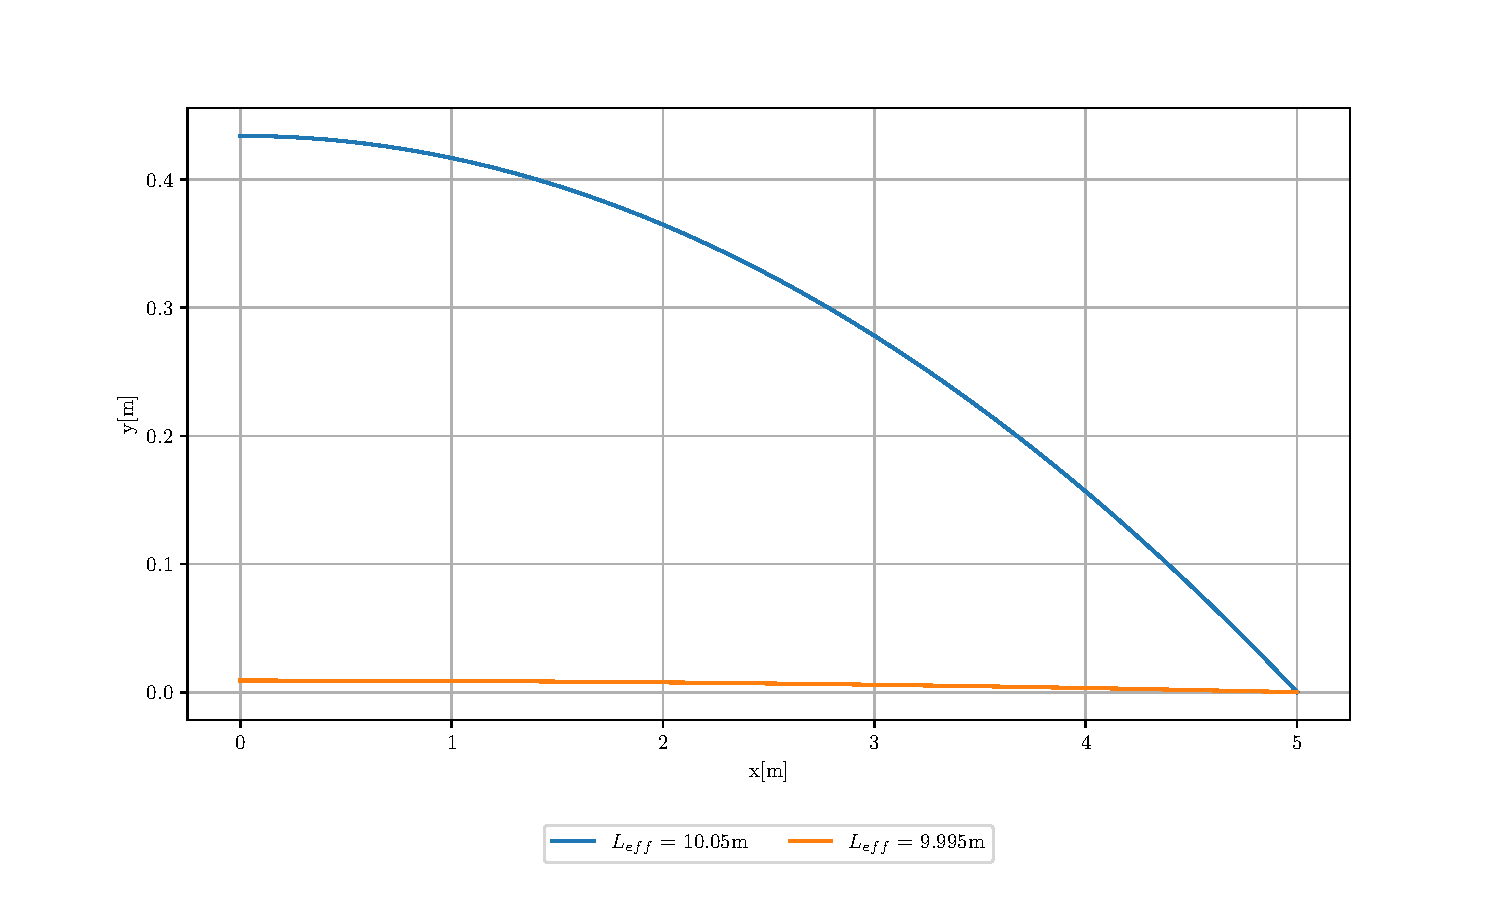
\includegraphics[width=\textwidth]{143_capitoli/capitolo2/immagini_capitolo_2/differenzevsestensibile1.pdf}
    \caption{Deformata di funi soggette al peso proprio ottenuta con il metodo delle differenze finite}
    \label{fig:differenzevsestensibile1}
\end{figure}

\begin{figure}[H]
    \centering
    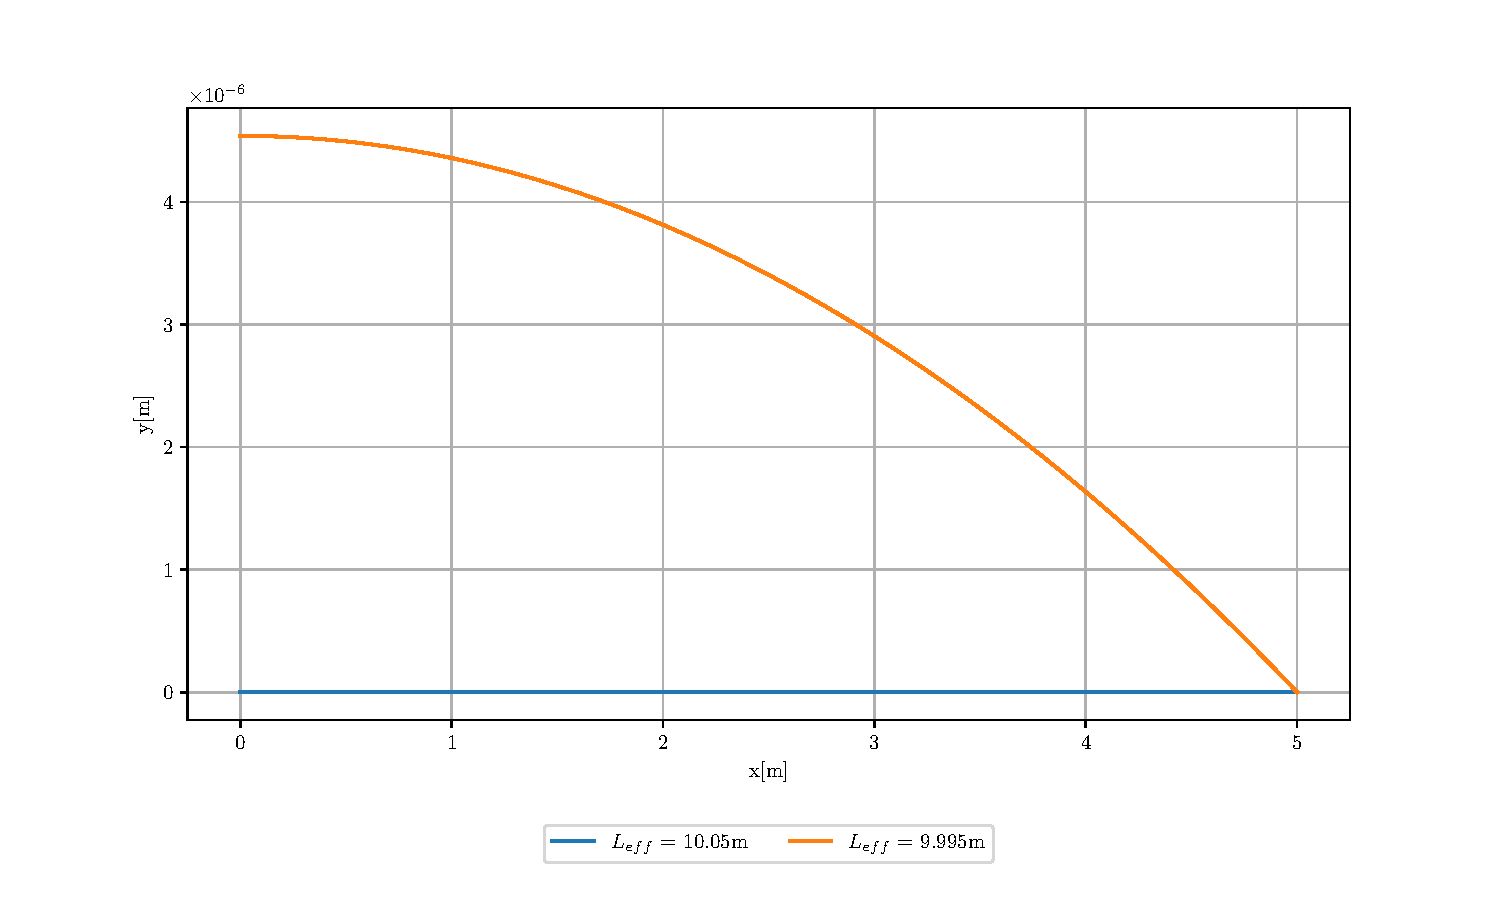
\includegraphics[width=\textwidth]{143_capitoli/capitolo2/immagini_capitolo_2/differenzevsestensibile2.pdf}
    \caption{Errore assoluto: catenaria estensibile vs metodo delle differenze finite}
    \label{fig:differenzevsestensibile2}
\end{figure}


\section{Sviluppo di un modello agli elementi finiti}
Data l'inesistenza di una teoria che conduca a soluzioni analitiche per il problema delle reti di funi, si rende necessario l'impiego di un metodo numerico di approssimazione. 

Una rete comprende funi annodate e attorcigliate su loro stesse a formare una struttura flessibile con geometria a griglia. Questa configurazione si presta ad una discretizzazione della risposta meccanica in funi e nodi: la rete può essere modellata come un sistema discreto di $m$ funi, connesse a $n$ nodi come schemattizzato in \cref{fig:rete_discretizzata1}. 

\begin{figure}[htbp]
  \centering
  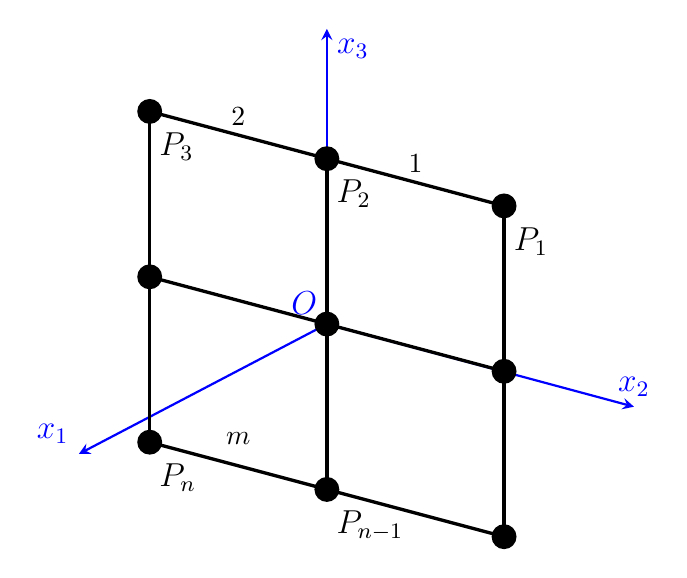
\begin{tikzpicture}[scale=1.5, >=stealth, every node/.style={scale=1.0}]

    % Coordinate dei nodi della griglia (prospettiva isometrica/3D semplificata)
    % Riga superiore
    \coordinate (P3) at (-1.5, 1.8);
    \coordinate (P2) at (0, 1.4);
    \coordinate (P1) at (1.5, 1.0);
    
    % Riga centrale
    \coordinate (M3) at (-1.5, 0.4);
    \coordinate (O)  at (0, 0);
    \coordinate (M1) at (1.5, -0.4);
    
    % Riga inferiore
    \coordinate (Pn)   at (-1.5, -1.0);
    \coordinate (Pn1)  at (0, -1.4);
    \coordinate (B1)   at (1.5, -1.8);

    % --- ASSI CARTESIANI (In blu, posizionati sotto i nodi per non sovrapporsi graficamente) ---
    \draw[blue, thick, ->] (O) -- (-2.1, -1.1) node[above left, font=\large] {$x_1$};
    \draw[blue, thick, ->] (O) -- (2.6, -0.7) node[above, font=\large] {$x_2$};
    \draw[blue, thick, ->] (O) -- (0, 2.5) node[below right, font=\large] {$x_3$};
    
    % Origine degli assi
    \node[blue, above left, font=\large\bfseries] at (O) {$O$};

    % --- LINEE DELLA RETE (Funi) ---
    % Linee orizzontali (corde)
    \draw[very thick, black] (P3) -- (P2) -- (P1);
    \draw[very thick, black] (M3) -- (O) -- (M1);
    \draw[very thick, black] (Pn) -- (Pn1) -- (B1);
    
    % Linee verticali (montanti)
    \draw[very thick, black] (P3) -- (M3) -- (Pn);
    \draw[very thick, black] (P2) -- (O) -- (Pn1);
    \draw[very thick, black] (P1) -- (M1) -- (B1);

    % --- NODI (Cerchi neri) ---
    \foreach \nodo in {P3, P2, P1, M3, O, M1, Pn, Pn1, B1} {
        \fill[black] (\nodo) circle (3.0pt);
    }

    % --- ETICHETTE DEI NODI E DEGLI ELEMENTI ---
    % Nodi superiori
    \node[below right, font=\large] at (-1.5, 1.7) {$P_3$};
    \node[below right, font=\large] at (0, 1.3) {$P_2$};
    \node[below right, font=\large] at (1.5, 0.9) {$P_1$};
    
    % Nodi inferiori
    \node[below right, font=\large] at (-1.5, -1.1) {$P_n$};
    \node[below right, font=\large] at (0, -1.5) {$P_{n-1}$};
    
    % Numerazione elementi (sopra le campate)
    \node[above, font=\normalsize] at (-0.75, 1.6) {$2$};
    \node[above, font=\normalsize] at (0.75, 1.2) {$1$};
    \node[above, font=\normalsize] at (-0.75, -1.1) {$m$};

\end{tikzpicture}
  \caption{Possibile modello di discretizzazione della rete }
  \label{fig:rete_discretizzata1}
\end{figure}

Masse, proprietà elastiche, carichi applicati e vincoli sono trattati come entità concentrate. Descrivendo la deformazione delle funi in accordo con opportune funzioni di forma, il modello si allinea pienamente con il Metodo degli Elementi Finiti (FEM).

La concezione di questo metodo non varia in funzione della spazialità del problema e la formulazione non distingue i casi bidimensionali da quelli tridimensionali. Visto l'obiettivo finale, e non disponendo di teorie analitiche sull'intera rete, l'accuratezza del codice verrà verificata confrontando i risultati del FEM con le risposte analitiche relative alla singola fune.

Nelle reti a maglie poligonali, la pratica comune prevede di posizionare i nodi del modello alle intersezioni tra le funi defininendo gli elementi come le porzioni di fune incluse tra di essi. Sebbene questo approccio sia molto diffuso nei modelli discreti, sono possibili strategie differenti in funzione della scala del problema strutturale. Quando si considerano reti di dimensioni importanti, quali le reti di sicurezza o le reti anticalcinacci, la struttura reale può comprendere diverse centinaia di migliaia di nodi. In questi casi per rendere computazionalmente fattibile l'analisi numerica, più maglie possono essere approssimate come una sola; di conseguenza i nodi e gli elementi del modello meccanico non corrisponderanno sempre ai nodi ed ai fili reali della rete. Nel caso opposto, una singola fune può essere discretizzata in un numero arbitrario di elementi finiti, così da rappresentarne accuratamente la curvatura e il comportamento geometrico non lineare. Quest'ultima strategia verrà sfruttata nel corso delle trattazione proprio per confrontare i risultati ottenuti dal codice con quelli analitici della catenaria elastica. 

\subsection{Position-based Finite Element Formulation}

Proponiamo un modello agli elementi finiti (FE) di reti di funi con masse nodali concentrate e elementi $cavo$ del primo ordine. In linea con il position-based finite element formulation (PFEF) \cite{Valvo1}\cite{Valvo2}, assumiamo come incognite principali del problema le posizioni nodali, anzichè gli spostamenti nodali, che sono comunemente adottati nelle analisi agli elementi finiti. Come risultato, la matrice di rigidezza elastica secante del sistema risulterà essere simmetrica e non sarà necessaria l'adozione di due distinti sistemi di riferimento (locale e globale), in quanto ogni grandezza è riferita a un unico sistema di coordinate globali. 

I grandi spostamenti e le deformazioni finite sono descritte per mezzo del tensore di deformazione di Green-Lagrange. si assume che gli elementi cavo possano reagire solamente in trazione ($tension-only$) mediante una relazione lineare tra la deformazione assiale e la corrispondente componente del secondo tensore delle tensioni di Piola-Kirchhoff. Questa legge costitutiva è nota in letteratura come modello di materiale di Saint-Venant-Kirchhoff. 

\vspace{1em}
Le configurazioni di riferimento e corrente sono definite rispetto al sistema di riferimento cartesiano $Ox_{1}x_{2}x_{3}$, illustrato in figura \cref{fig:rete_discretizzata1}. Indicando rispettivamente con $\overline{\Omega}$ e $\Omega$ il dominio del sistema meccanico nella configurazione di riferimento e in quella corrente, da qui in avanti tutte le grandezze geometriche e meccaniche relative alla configurazione di riferimento saranno contrassegnate dall'overline; viceversa le quantità prive di barra sarnno riferite alla configurazione corrente. Sia $P_i$ la posizione dell'$i$-esimo nodo $(i = 1,\dots,n)$ nella configurazione corrente e $\overline{P}_i$ la medesima posizione nella configurazione di riferimento, la quale per definizione viene assunta geometricamente indeformata. Il vettore posizione del generico nodo in configurazione corrente è definito come $\underline{x}_i = P_i - O \in \mathbb{R}^3 $, mentre il corrispondente vettore spostamento può essere espresso mediante la relazione $\underline{u}_i = P_i - \overline{P}_i$. Infine, raccogliendo i vettori posizione di tutti gli $n$ nodi del sistema in un unico vettore globale delle coordiante nodali $x \in \mathbb{R}^{3n}$, quest'ultimo viene assunto come la principale incognita cinematica del problema strutturale. 

\subsection{L'elemento cavo}
Consideriamo l'$e-esimo$ elemento $(e = 1,\dots,m)$ che connette l'$i-esimo$ e $j-esimo$ nodo come rappresentato in \cref{fig:elementocavo}. Indichiamo il vettore delle posizioni nodali dell'elemento in configurazione corrente come $\underline{x}_e = [\underline{x}_i ; \underline{x}_j] \in \mathbb{R}^6$. La lunghezza nominale dell'elemento $l_e$, è definita come la distanza tra i suoi nodi, e potrà essere calcolata con la seguente formula: 

\begin{figure}[htbp]
  \centering
  \begin{tikzpicture}[
    % Definizione degli stili grafici per il disegno
    cable/.style={double=blue!50, double distance=2.5pt, thick, line cap=squared},
    vector/.style={-{Stealth[scale=1.2]}, blue, thick},
    dimline/.style={black, thin},
    dot/.style={circle, fill=black, inner sep=1.5pt}
]

% ==================== CONFIGURAZIONE A) SLACK ELEMENT ====================
\begin{scope}[shift={(0,0)}]
    % Coordinate della configurazione di riferimento
    \coordinate (Pibar) at (0,0);
    \coordinate (Pjbar) at (5,0);
    \coordinate (Pbar) at (2.8,0);
    
    % Disegno elemento di riferimento (barra inferiore)
    \draw[cable] (Pibar) -- (Pjbar);
    
    % Coordinate della configurazione corrente (cavo allentato)
    \coordinate (Pi) at (0.3,1.6);
    \coordinate (Pj) at (4.3,2.2);
    \coordinate (P) at (2.4,1.7);
    
    % Vettori di spostamento (frecce blu)
    \draw[vector] (Pibar) -- (Pi) node[midway, right, yshift=2pt] {$\underline{u}_i$};
    \draw[vector] (Pjbar) -- (Pj) node[midway, left] {$\underline{u}_j$};
    \draw[vector] (Pbar) -- (P) node[midway, right] {$\underline{u}_P$};
    
    % Cavo in configurazione "Slack" (curve morbide di Bezier)
    \draw[cable] (Pi) .. controls (1.0,2.0) and (1.5,2.7) .. (1.8,2.7)
                      .. controls (2.1,2.7) and (1.6,1.3) .. (1.8,1.35)
                      .. controls (1.9,1.4) and (2.2,1.7) .. (P)
                      -- (Pj);
                      
    % Etichette di nodi e regioni
    \node[left, xshift=-2pt] at (Pibar) {$\bar{P}_i$};
    \node[right, xshift=2pt] at (Pjbar) {$\bar{P}_j$};
    \node[above right, xshift=-2pt] at (Pbar) {$\bar{P}$};
    \node[above, yshift=2pt] at ($(Pibar)!0.4!(Pjbar)$) {$\bar{\Omega}_e$};
    
    \node[above left] at (Pi) {$P_i$};
    \node[above right] at (Pj) {$P_j$};
    \node[above right, yshift=2pt] at (P) {$P$};
    \node[above, xshift=-4pt] at (1.1,2.0) {$\Omega_e$};
    
    % Quota inferiore per \bar{l}_e
    \draw[dimline] (0,0) -- (0,-1.2);
    \draw[dimline] (5,0) -- (5,-1.2);
    \draw[dimline] (0,-1.0) -- (5,-1.0) node[midway, fill=white] {$\bar{l}_e$};
    \node[dot] at (0,-1.0) {};
    \node[dot] at (5,-1.0) {};
    
    % Quota superiore parallela per l_e
    \coordinate (L1) at ($(Pi) + (-0.4, 1.1)$);
    \coordinate (L2) at ($(Pj) + (-0.4, 1.1)$);
    \draw[dimline] (Pi) -- (L1);
    \draw[dimline] (Pj) -- (L2);
    \draw[dimline] (L1) -- (L2) node[midway, fill=white] {$l_e$};
    \node[dot] at (L1) {};
    \node[dot] at (L2) {};
    
    % Didascalia grafica a)
    \node[below] at (2.5,-1.6) {(a) elemento lasco};
\end{scope}

% ==================== CONFIGURAZIONE B) TENSE ELEMENT ====================
\begin{scope}[shift={(7.5,0)}] % Traslato a destra per affiancarlo a quello sopra
    % Coordinate di riferimento
    \coordinate (Pibar) at (0,0);
    \coordinate (Pjbar) at (5,0);
    \coordinate (Pbar) at (3.5,0);
    
    \draw[cable] (Pibar) -- (Pjbar);
    
    % Coordinate configurazione corrente (rettilineo teso)
    \coordinate (Pi) at (0,2.2);
    \coordinate (Pj) at (4.7,0.8);
    \coordinate (P) at (3.2,1.25);
    
    % Vettori di spostamento (frecce blu)
    \draw[vector] (Pibar) -- (Pi) node[midway, left] {$\underline{u}_i$};
    \draw[vector] (Pjbar) -- (Pj) node[midway, left, xshift=-1pt] {$\underline{u}_j$};
    \draw[vector] (Pbar) -- (P) node[midway, left] {$\underline{u}_P$};
    
    % Cavo teso (linea retta)
    \draw[cable] (Pi) -- (Pj);
    
    % Etichette
    \node[left, xshift=-2pt] at (Pibar) {$\bar{P}_i$};
    \node[right, xshift=2pt] at (Pjbar) {$\bar{P}_j$};
    \node[above right, xshift=-2pt] at (Pbar) {$\bar{P}$};
    \node[above, yshift=2pt] at ($(Pibar)!0.3!(Pjbar)$) {$\bar{\Omega}_e$};
    
    \node[above left] at (Pi) {$P_i$};
    \node[above right] at (Pj) {$P_j$};
    \node[above right] at (P) {$P$};
    \node[above] at ($(Pi)!0.3!(Pj)$) {$\Omega_e$};
    
    % Quota inferiore per \bar{l}_e
    \draw[dimline] (0,0) -- (0,-1.2);
    \draw[dimline] (5,0) -- (5,-1.2);
    \draw[dimline] (0,-1.0) -- (5,-1.0) node[midway, fill=white] {$\bar{l}_e$};
    \node[dot] at (0,-1.0) {};
    \node[dot] at (5,-1.0) {};
    
    % Quota superiore parallela per l_e
    \coordinate (L1) at ($(Pi) + (0.4, 1.1)$);
    \coordinate (L2) at ($(Pj) + (0.4, 1.1)$);
    \draw[dimline] (Pi) -- (L1);
    \draw[dimline] (Pj) -- (L2);
    \draw[dimline] (L1) -- (L2) node[midway, fill=white] {$l_e$};
    \node[dot] at (L1) {};
    \node[dot] at (L2) {};
    
    % Didascalia grafica b)
    \node[below] at (2.5,-1.6) {(b) elemento teso};
\end{scope}

\end{tikzpicture}
  \caption{Elementi cavo in configurazione di riferimento e corrente}
  \label{fig:elementocavo}
\end{figure}


\begin{equation}
   l_e^2 = \left( \underline{x}_j - \underline{x}_i \right)^2 =  \underline{x}_e^T 
   \begin{bmatrix}
    I & -I \\
    -I &  I 
   \end{bmatrix} \underline{x}_e
   \label{eq:lunghezza_elemento_quadro}
\end{equation}
dove $I \in \mathbb{R}^{3x3}$ è la matrice identità. La componente del tensore delle deformazioni di Green-Lagrange nella direzione assiale dell'elemento è valutata rispetto alla configurazione di riferimento come: 
\begin{equation}
   e_{11} = \frac{1}{2}\frac{l_e^2 - \overline{l}_e^2}{\overline{l}_e^2}
   \label{eq:deformazione_green_lagrange}
\end{equation}
La tensione nella direzione assiale dell'elemento è ottenuta per mezzo della legge costitutiva che tiene conto dell'impossibilità dei cavi di sostenere sforzi di compressione (dovuto all'instabilità causata dalla scarsa rigidezza flessionale delle funi). Quando la lunghezza nominale corrente dell'elemento è inferiore alla lunghezza di riferimento, l'elemento si considera lasco ($slack$) e lo sforzo normale è da assumersi nullo. Negli altri casi si assume una relazione elastica lineare tra la deformazione di Green-Lagrange e la componente del secondo tensore di Piola-Kirchhoff:
\begin{equation}
   \sigma_{11} =
\begin{cases}
E \, e_{11}, & \text{se } e_{11} \geq 0 \\[6pt]
0, & \text{negli altri casi } 
\end{cases}
\label{eq:tension_only2}
\end{equation}
dove $E$ è il modulo di Young del materiale. 

Assumendo delle funzioni di forma lineari per gli elementi, in accordo con \cite{Valvo1,Valvo2}, la matrice di rigidezza elastica secante del singolo cavo $S_e \in \mathbb{R}^{6x6}$ può essere espressa mediante la relazione:
\begin{equation}
   S_e(\underline{x}_e) = \sigma_{11} \frac{\overline{a}_e}{\overline{l}_e}\begin{bmatrix}
    I & -I \\
    -I &  I 
   \end{bmatrix}
   \label{eq:matrice_secante}
\end{equation}
dove $\overline{a}_e$ è l'area della sezione dell'elemento, valutata in configurazione di riferimento. Allo stesso tempo, la matrice di rigidezza elastica tangente $T_e \in \mathbb{R}^{6x6}$ si ottiene differenziando le forze interne e può essere espressa come:
\begin{equation}
   T_e\left(\underline{x}_e\right) = S_e\left(\underline{x}_e\right) + \frac{\partial \sigma_{11}}{\partial e_{11}}\frac{\overline{a}_e l_e^2}{\overline{l}_e^3} \left[\begin{matrix}
    I & -I \\
    -I &  I  
   \end{matrix}\right]
\label{eq:matrice_tangente}
\end{equation}  
che, secondo quanto dimostrato in \cite{Fisicaro} può essere riscritta in forma compatta come: 
\begin{equation}
   T_e\left(\underline{x}_e\right) = \left(\sigma_{11} + \frac{\partial \sigma_{11}}{\partial e_{11}}\frac{l_e^2}{\overline{l}_e^2}\right) \frac{\overline{a}_e}{\overline{l}_e} \left[\begin{matrix}
    I & -I \\
    -I &  I  
   \end{matrix}\right]
\label{eq:matrice_tangente2}
\end{equation}  
Dalle equazioni \eqref{eq:matrice_secante} e \eqref{eq:matrice_tangente2} la dipendenza esplicita delle matrici dal vettore delle posizioni nodali dell'elemento $\underline{x_e}$ è racchiusa implicitamente nella lunghezza nominale $l_e$. 

\vspace{1em}
Come detto in precedenza, il modello a massa concentrata adottato prevede di ripartire la massa totale dell'elemento sui nodi di estremità. In accordo con la formulazione classica di \cite{Penzien}, assumiamo per il singolo elemento la seguente matrice di massa globale $M_e \in \mathbb{R}^{6x6}$:
\begin{equation}
   M_e = 
   \frac{1}{2}\ \overline{\rho}_e\,\overline{a}_e\,\overline{l}_e 
   \begin{bmatrix}
      I & 0 \\
      0 & I
   \end{bmatrix}
\end{equation}
dove $\overline{\rho}_e$ è la densità di massa uniforme nella configurazione di riferimento, e $0 \in \mathbb{R}^{3x3}$ è la sottomatrice nulla. La struttura diagonale a blocchi riflette il fatto che ciascun nodo riceve metà della massa totale dell'elemento, senza accoppiamenti inerziali reciproci. 

Nel caso di problemi statici, il contributo inerziale è trascurabile. L'unico effetto della massa è legato alla forza peso. Per questo motivo, anzichè assemblare l'intera matrice di massa del sistema, si introduce direttamente il vettore di carico gravitazionale dell'elemento $f_{g,e} \in \mathbb{R}^6$:
\begin{equation}
   \underline{f}_{g,e} = \frac{1}{2}\overline{\rho}_e \overline{a}_e \overline{l}_e g
\left\{
\begin{array}{c}
0 \\
0 \\
1 \\
0 \\
0 \\
1 \\
\end{array}
\right\}
\end{equation}
dove $g$ è l'accelerazione gravitazionale. Il vettore rappresenta la forza peso applicata ai due nodi dell'elemento, orientata lungo la direzione verticale del sistema di riferimento (assumendo l'asse $x_3$ rivolto verso il basso).  

\vspace{1em}
Al fine di formalizzare l'assemblaggio delle matrici appena introdotte e relative all'intero sistema meccanico introduciamo la matrice di localizzazione dell'$i-esimo$ nodo $L_i \in \mathbb{R}^{3x3n}$ e la matrice di assemblaggio dell'$e-simo$ elemento $A_e \in \mathbb{R}^{6x3n}$. 
La matrice di localizzazione è definita come una matrice nulla, eccetto per le componenti corrispondenti alle colonne da $3i -2$ a $3i$ dove è posizionata la matrice identità $I \in \mathbb{R}^{3x3}$ .
\begin{equation}
   L_i = 
   \begin{bmatrix}
      0 & \dots & 0 & I & 0 & \dots & 0 
   \end{bmatrix}
   \label{eq:matrice_localizzazione}
\end{equation}
La matrice di localizzazione può essere usata per estrarre il vettore posizione dell'i-esimo nodo a partire dal vettore globale, ossia $\underline{x}_i = L_i \underline{x}$. Di conseguenza, l'operatore trasposto permette di scrivere $\underline{x} = \sum_{i=1}^{n} L_i^T \underline{x}_i$.
La matrice di assemblaggio dell'elemento $e$, che connette i nodi $i$ e $j$, si ottiene affiancando verticalmente le matrici di localizzazione dei suoi nodi di estremità: 
 \begin{equation}
   A_e = 
   \begin{bmatrix}
      L_i \\
      L_j   
   \end{bmatrix}=
   \begin{bmatrix}
      0 & \dots & 0 & I & 0 & \dots & 0 & 0 & 0 \dots & 0 \\
      0 & \dots & 0 & 0 & 0 & \dots & 0 & I & 0 \dots & 0 \\
   \end{bmatrix}
   \label{eq:matrice_assemblaggio}
\end{equation} 
Di fatto la matrice di assemblaggio raccoglie le matrici di localizzazione dei due nodi di estremità dell'elemento. Come risultato, il vettore delle posizioni nodali dell'elemento potrà essere espresso come $\underline{x}_e = A_e \underline{x}$.
Come risultato, il vettore delle posizioni nodali dell'elemento può essere espresso in funzione del vettore globale $\underline{x}_e = A_e \underline{x}$. 

\subsection{La rete di funi}
Il vettore globale delle forze peso dell'intera rete $f_g \in \mathbb{R}^{3n}$ è ottenuto sommando i contributi dei singoli elementi tramite le rispettive matrici di assemblaggio trasposte:
\begin{equation}
 \underline{f}_{g,e} = \sum_{e=1}^{m} A_e^T \underline{f}_{g,e}
 \label{eq:vettore_peso}
\end{equation}
Le matrici di rigidezza elastica secante $S(\underline{x})$ e tangente $T(\underline{x})$ dell'intera rete, appartenenti a $\mathbb{R}^{3 \times 3n}$ si ricavano per assemblaggio diretto:
\begin{equation}
   \begin{aligned}
   S(\underline{x}) = \sum_{e=1}^{m} A_e^T S_e(\underline{x}_{e})A_e\\
   T(\underline{x}) = \sum_{e=1}^{m} A_e^T T_e(\underline{x}_{e})A_e
    \end{aligned}
   \label{eq:matrice_rigidezza}
\end{equation}
Per trattare il problema in via generale, definiamo la matrice di massa globale dell'intera struttura $M \in \mathbb{R}^{3n \times 3n}$: 
\begin{equation}
   M = \sum_{e=1}^{m} A_e^T M_e A_e
   \label{eq:matrice_massa}
\end{equation}
Infine, introduciamo lo smorzamento nel modello secondo le ipotesi di Rayleigh \cite{Penzien}. La matrice di smorzamento $D \in \mathbb{R}^{3n \times 3n}$ è ottenuta come la combinazione lineare della matrice di massa e della matrice di rigidezza elastica tangente, quest'ultima valutata nella configurazione di riferimento (o indeformata) $\underline{\overline{x}}$: 
\begin{equation}
   D = \alpha_d M + \beta_d T(\underline{\overline{x}})
   \label{eq:matrice_smorzamento}
\end{equation}
dove $\alpha_d$ e $\beta_d$ sono coefficienti di proporzionalità di Rayleigh.

\subsection{La formulazione lagrangiana}
Le equazioni differenziali che governano il problema dell'equilibrio dinamico non lineare possono essere dedotte secondo appocci differenti. In accordo con \cite{Fisicaro}, seguiamo il metodo Lagrangiano. Lo stesso approccio sarà adottato successivamente per trattare il problema di contatto tra una rete ed un oggetto.

Definiamo la funzione Lagrangiana $\mathcal{L}$ del sistema come la differenza tra l'energia cinetica $\mathcal{K}$ e l'energia potenziale totale $\mathcal{V}$:
\begin{equation}
   \mathcal{L}(\underline{x}, \underline{\dot{x}}, t) = \mathcal{K} - \mathcal{V}
   \label{eq:funzione_lagrangiana}
\end{equation}
con $\mathcal{L}: \mathbb{R}^{6n+1} \rightarrow \mathbb{R}$. Il punto sovrapposto indica la derivazione rispetto al tempo $t$ del vettore $\underline{x}$. 

L'energia cinetica globale del sistema discreto può essere ottenuta dalla sua definizione: 
\begin{equation}
   \mathcal{K} = \frac{1}{2} \underline{\dot{x}}^T M \underline{\dot{x}}
   \label{eq:energia_cinetica}
\end{equation}
L'energia potenziale totale $\mathcal{V}$ racchiude i contributi associati alle forze conservative, tra cui il potenziale della forza peso e l'energia potenziale elastica interna $\mathcal{U}$.

\subsubsection{L'energia potenziale elastica}
L'energia potenziale elastica dell'$e-esimo$ elemento si esprime come \cite{Valvo1,Valvo2}: 
\begin{equation}
   \mathcal{U}_e = \int_{\overline{\Omega}_e} \overline{\varphi}\, dx1dx2dx3
\end{equation}
Dove $\overline{\varphi}$ è la densità di energia di deformazione elastica per unità di volume nella configurazione di riferimento. Per l'elemento cavo considerato nel modello, $\mathcal{U}_e$ ha l'espressione analitica: 
\begin{equation}
   \mathcal{U}_e = \frac{1}{2} \sigma_{11} e_{11} \overline{a}_e \overline{l}_e
\end{equation}
L'energia potenziale elastica totale dell'intero sistema meccanico è la somma dei contributi sui singoli elementi: 
\begin{equation}
   \mathcal{U} = \frac{1}{2} \sum_{e=1}^{m} \sigma_{11} e_{11} \overline{a}_e \overline{l}_e
   \label{eq:energia_potenziale_elastica}
\end{equation}
Ricordando le equazioni \eqref{eq:deformazione_green_lagrange} e \eqref{eq:tension_only2} si arriva all'espressione: 
\begin{equation}
   \frac{\partial (\sigma_{11} e_{11})}{\partial {\underline{x}}} = 2\sigma_{11} \frac{\partial e_{11}}{\partial {\underline{x}}} = \frac{\sigma_{11}}{\overline{l}_e^2} \frac{\partial l_e^2}{\partial {\underline{x}}}
\end{equation}
Differenziando l'energia potenziale del singolo elemento rispetto al vettore delle posizioni globali $\underline{x}$, otteniamo:
\begin{equation}
   \frac{\partial \mathcal{U}}{\partial {\underline{x}}} = \frac{1}{2} \sum_{e=1}^{m} \overline{a}_e \overline{l}_e \frac{\partial {\sigma_{11} e_{11}}}{\partial {\underline{x}}} = \frac{1}{2} \sum_{e=1}^{m} \sigma_{11} \frac{\overline{a}_e}{\overline{l}_e} \frac{\partial l_e^2}{\partial {\overline{x}}}
   \label{eq:derivata_energia_potenziale_elastica}
\end{equation}
Dall'equazione \ref{eq:lunghezza_elemento_quadro} segue la relazione: 
\begin{equation}
   \frac{\partial l_e^2}{\partial{\underline{x}}} = \frac{\partial}{\partial{\underline{x}}} \left\{ \underline{x}_e^T 
   \begin{bmatrix}
    I & -I \\
    -I &  I 
   \end{bmatrix} \underline{x}_e \right\}
\end{equation}
che, sfruttando la matrice di assemblaggio e scrivendo $\underline{x}_e = A_e \underline{x}$, diventa: 
\begin{equation}
   \frac{\partial l_e^2}{\partial{\underline{x}}} = \frac{\partial}{\partial{\underline{x}}} \left\{ \underline{x}^T A_e^T
   \begin{bmatrix}
    I & -I \\
    -I &  I 
   \end{bmatrix} A_e \underline{x} \right\} = 2 A_e^T \begin{bmatrix}
    I & -I \\
    -I &  I 
   \end{bmatrix} 
   A_e \underline{x}
   \label{eq:derivata_lunghezza_elemento}
\end{equation}
Sostituendo l'equazione \eqref{eq:derivata_lunghezza_elemento} in \eqref{eq:derivata_energia_potenziale_elastica} otteniamo il seguente risultato: 
\begin{equation}
   \frac{\partial {\mathcal{U}}}{\partial {\underline{x}}} = \sum_{e=1}^{m} \sigma_{11} \frac{\overline{a}_e}{\overline{l}_e} A_e^T \begin{bmatrix}
    I & -I \\
    -I &  I 
   \end{bmatrix} 
   A_e \underline{x}
\end{equation}
Confrontando tale risultato cone le definizioni delle matrici \eqref{eq:matrice_secante} e \eqref{eq:matrice_rigidezza}, il gradiente dell'energia potenziale elastica corrisponde esattamente al vettore delle forze interne elastiche globali del sistema: 
\begin{equation}
   \frac{\partial {\mathcal{U}}}{\partial {\underline{x}}} = S (\underline{x}) \underline{x}
\end{equation}

\subsubsection{Il contributo dissipativo}
Per tener conto delle forze dissipative, estendiamo il formalismo lagrangiano introducendo la funzione di dissipazione di Rayleigh \cite{Penzien}:
\begin{equation}
   \mathcal{R} = \frac{1}{2} \underline{\dot{x}}^T D \underline{\dot{x}}
   \label{eq:dissipazione}
\end{equation}
La funzione di dissipazione di Rayleigh esprime la perdita di potenza nel sistema meccanico causata dalle forze non conservative.

\subsubsection{Equazioni di governo}
L'espressione generale dell'equazione lagrangiana è la seguente: 
\begin{equation}
   \frac{d}{dt} \left( \frac{\partial \mathcal{L}}{\partial \dot{x}_h}\right) - \frac{\partial \mathcal{L}}{\partial  x_h} = \frac{\partial \mathcal{R}}{\partial \dot{x}_h} + p_h
\end{equation}
dove $p_h$ rappresenta la componente della forza generalizzata non conservativa ed esterna non inclusa nel potenziale.
Sostituendo le espressioni ricavate e sviluppando le derivate, arriviamo al sistema di equazioni differenziali ordinarie del secondo ordine, non lineare, che governa la dinamica della rete: 
\begin{equation}
   M \ddot{\underline{x}} + D \dot{\underline{x}} + S(\underline{x}) \underline{x} = \underline{p}
   \label{eq:equilibrio_dinamico_problema}
\end{equation}
In questa formulazione, sia il vettore delle posizioni dei nodi $\underline{x}(t)$ che il vettore dei carichi nodali esterni globali $\underline{p}(t)$, dipendono dal tempo. 

\subsubsection{I problemi statico e quasti statico}
L'equazione fondamentale di equilibrio statico o quasi-statico può essere ricavata come caso degenerato dell'equazione generalizzata \eqref{eq:equilibrio_dinamico_problema}
Nel caso statico, le azioni esterne sono costanti nel tempo $\underline{p}(t) = p_0$. Le accelerazioni e le velocità sono identicamente nulle ($\ddot{\underline{x}} = 0, \dot{\underline{x}} = 0$). Di conseguenza, il sistema di equazioni differenziali si riduce a un sistema di equazioni algebriche non lineari in cui la variabile tempo scompare esplicitamente:
\begin{equation}
   S(\underline{x}) \underline{x} = \underline{p}
   \label{eq:problema_statico}
\end{equation}
Nel caso quasi-statico, le azioni esterne variano nel tempo in modo sufficientemente lento da non far nascere effetti inerziali o dissipativi significativi. Sotto questa ipotesi, le derivate temporali restano trascurabili ($\ddot{\underline{x}} \approx 0, \dot{\underline{x}} \approx 0$), ma lo stato di deformazione segue l'evoluzione cronologica del carico. L'equilibrio istante per istante è governato dalla relazione: 
\begin{equation}
   S(\underline{x}(t)) \underline{x}(t) = \underline{p}(t)
   \label{eq:problema_quasi_statico}
\end{equation}

\subsection{Un'applicazione: la fune soggetta al peso proprio}
Applichiamo la formulazione PFEF specializzata al caso bidimensionale per lo studio di una singola fune soggetta al peso proprio. Ciò consentirà di paragonare i risultati numerici del modello FEM con quelli ottenuti tramite la soluzione analitica della catenaria elastica la quale, come mostrato in precedenza, approssima accuratamente la soluzione del problema differenziale mediante il metodo delle differenza finite.

E' opportuno precisare che tale confronto mira ad evidenziare le differenze intrinseche tra i due approcci e non a validare due soluzioni identiche dello stesso problema. Infatti, a differenza del modello analitico della catenaria elastica, che utilizza un'approssimazione al primo ordine dell'allungamento, l'approccio FEM qui descritto impiega la componente assiale del tensore di deformazione di Green-Lagrange; pertanto, i due modelli risultano teoricamente distinti. 

\vspace{1em}
Sebbene la formulazione del PFEF sia stata presentata nel dominio tridimensionale per preservare la generalità, il problema cinematico della singola fune soggetta al peso proprio può essere convenientemente studiato nel piano verticale $Ox_1x_3$. In assenza di carichi ortogonali a tale piano e assumendo una configurazione di riferimento contenuta in esso, la terza componente dello spostamento e della posizione di ogni nodo risulta identicamente nulla. 

Di conseguenza, è possibile ridurre lo spazio delle incongnite eliminando i gradi di libertà associati all'asse $x_2$. Il vettore posizione del generico nodo $i$-esimo si riduce a $\underline{x}_i = [x_{1,i}, x_{3,i}] \in \mathbb{R}^{2}$, e il vettore globale delle coordiante nodali apparterrà allo spazio $\underline{x} \in \mathbb{R}^{2n}$.
Dal punto di vista dell'implementazione numerica, le matrici identità $I$ e nulle $0$ presenti nella definizioni degli elementi e degli operatori di assemblaggio, quali la lunghezza dell'elemento \eqref{eq:lunghezza_elemento_quadro}, le matrici di rigidezza \eqref{eq:matrice_secante} e \eqref{eq:matrice_tangente}, vengono ridotte da dimensioni $3 \times 3$ a dimensioni $2 \times 2$. Questa riduzione non altera la struttura algebrica delle equazioni di governo, ma dimezza il numero di incognite totali, ottimizzando significativamente l'efficienza computazionale del solutore non lineare.

\vspace{1em}
Il problema meccanico della fune nel piano è descritto dalla relazione di equilibrio statico \eqref{eq:problema_statico}. In questo contesto, il vettore delle forze esterne $\underline{p}$ coincide con il vettore globale delle forze peso $\underline{f}_{g} \in \mathbb{R}^{2n}$, ottenuto per la fune discretizzata in $m$ elementi e $n$ nodi mediante la relazione \eqref{eq:vettore_peso}, dove la componente gravitazionale agisce esclusivamente lungo l'asse verticale $x_3$.

Il problema così delineato presenta una doppia non linearità: geometrica, dovuta al regime di grandi spostamenti, e costitutiva, legata all'introduzione del legame di tipo \textit{tension-only}. Per risolvere il sistema di equazioni algebriche non lineari, si impiega l'algoritmo iterativo di Newton-Raphson. Il vettore dei residui $R(\underline{x}) \in \mathbb{R}^{2n}$ è definito dalla relazione: 
\begin{equation}
   R(\underline{x}) = S(\underline{x})\underline{x} - \underline{f}_{g}
   \label{eq:residuo_problema_statico}
\end{equation}
La formula di ricorrenza dell'algoritmo, introdotta in generale nell'espressione \eqref{eq:ricorrenza_newton_raphson}, si specializza per questo caso come:
\begin{equation}
   \underline{x}^{(k+1)} = \underline{x}^{(k)} - [J(\underline{x}^{(k)})]^{-1} R(\underline{x}^{(k)})
\end{equation}
dove $[J(\underline{x}^{(k)})] \in \mathbb{R}^{2n \times 2n}$ è la matrice Jacobiana della funzione vettoriale del residuo $R(\underline{x})$. Poichè il vettore globale delle forze peso $\underline{f}_g$ dipende esclusivamente dalle proprietà geometriche e materiali definite nella configurazione di riferimento, esso risulta del tutto indipendente dallo stato cinematico corrente del sistema; la sua derivata rispetto alle posizioni attuali è pertanto nulla ($\partial f_{g,i} / \partial x_j = 0$).

Allo stesso tempo, il termine $\frac{\partial (S_i(\underline{x})\underline{x})}{\partial x_j}$ esprime la variazione del vettore delle forze interne elastiche globali rispetto alle coordinate correnti. Coerentemente con la formulazione introdotta in \cite{Fisicaro}, l'operazione di differenziazione del prodotto applicata al singolo elemento cavo mostra che la matrice di rigidezza tangente elementare $T_e$ è definita come la derivata prima del vettore delle forze elastiche nodali rispetto alle coordinate dei nodi stessi, sviluppata tramite la regola di derivazione delle funzioni composte:
\begin{equation}
   T_e(\underline{x}_e) = \frac{\partial (S_e \underline{x}_e)}{\partial \underline{x}_e} = S_e + \frac{\partial S_e}{\partial \underline{x}_e} \underline{x}_e
   \label{eq:rigidezza_meccanica_geometrica}
\end{equation}
Questo approccio analitico, basato sulla scomposizione della rigidezza tangente come somma del contributo secante attuale $S_e$ e del contributo dovuto alla variazione geometrica $\frac{\partial S_e}{\partial \underline{x}_e} \underline{x}_e$, si inserisce nel solco della letteratura classica ed è riportato in \cite{Fisicaro}. In tale ambito, si fa riferimento all'introduzione di $T_e$ nella soluzione con il metodo di Newton-Raphson dei problemi di elasticità non lineare, aventi come incognite le coordinate nodali, in accordo con \cite{Wriggers}.

\vspace{1em}
Nel caso specifico dell'elemento cavo qui trattato, introducendo il legame cinematico di Green-Lagrange \eqref{eq:deformazione_green_lagrange} e la legge costitutiva \textit{tension-only} \eqref{eq:tension_only2} all'interno del termine differenziale $\frac{\partial S_e}{\partial \underline{x}_e} \underline{x}_e$, l'esplicitazione di tale derivata conduce direttamente, come dimostrato in \cite{Fisicaro} nell'appendice A, alla formulazione compatta della matrice di rigidezza tangente elementare presentata nell'equazione \eqref{eq:matrice_tangente2}. In essa, la dipendenza dallo stato cinematico corrente rimane condensata implicitamente nel solo parametro della lunghezza nominale $l_e$.

Poichè l'operatore globale delle forze interne è ottenuto per assemblaggio lineare dei contributi dei singoli elementi tramite la relazione \eqref{eq:matrice_rigidezza}, la differenziazione del sistema globale coincide esattamente con la matrice di rigidezza tangente totale della rete, $T(\underline {x})$. Ne consegue che la matrice Jacobiana del problema statico equivalga alla matrice di rigidezza tangente globale, e le sue componenti possono essere espresse semplicemente come:
\begin{equation}
   J_{ij}(\underline{x}) = \frac{\partial (S_i(\underline{x})\underline{x})}{\partial x_j} = T_{ij}(\underline{x}),
   \qquad i,j = 1,\dots,2n.
   \label{eq:jacobiana_componenti2}
\end{equation}

\subsubsection{Il confronto tra le soluzioni al problema della fune elastica: analitica vs FEM }
Per confrontare i due approcci alla soluzione del problema della fune soggetta al peso proprio è stato scelto di prendere a riferimento i risultati relativi ad un elemento la cui distanza tra gli appoggi $l$ sia pari a $10m$ e la cui lunghezza effettiva in configurazione di riferimento $L_0$ sia di $10.05m$. Con $L_{eff}$ indichiamo invece la lunghezza assunta dalla fune a seguito dell'accorciamento $\Delta L_0$ in accordo con la relazione \eqref{eq:lunghezza_efficace}. In funzione del valore di $L_{eff}$ si distingueranno due casi, quello di cavo lasco (\textit{slack}) in cui $L_{eff}>l$ e quello di cavo teso $L_{eff}<l$. Questa differenziazione permetterà di evidenziare diversi aspetti tipici della trattazione FEM. 

In \cref{fig:deformate_PFEF} vengono mostrate le deformate di funi in configurazione sia lasca che tesa, mettendo direttamente a confronto la soluzione analitica classica e quella ottenuta tramite l'approccio numerico PFEF (utilizzando una mesh standard da 50 nodi). Da questa sovrapposizione grafica emerge l'ottima convergenza del solutore. Al fine di valutare rigorosamente l'accuratezza del codice sviluppato e interpretare i diagrammi degli errori locali (\cref{fig:errore_locale1_PFEF,fig:errore_locale2_PFEF}) e dello sforzo sforzo normale (\cref{fig:sforzonormale1_PFEF,fig:sforzonormale2_PFEF}), è possibile individuare tre distinte sorgenti di errore: 

\begin{itemize}
   \item Errore di convergenza del solutore: questa componente è intrinseca all'algoritmo iterativo di Newton-Raphson. La soluzione numerica si considera soddisfatta quando la norma del vettore residuo $\|R\| = \sqrt{\sum_{i=2}^{2n-3} R_i^2}$ (dove l'indice $i$ considera l'equilibrio dei soli gradi di libertà non vincolati del sistema) scende al di sotto di una determinata soglia. Mentre i valori standard di letteratura suggeriscono tolleranze comprese $10^{-5}$ e $10^{-7}$, nel presente lavoro si è adottato un criterio di convergenza restrittivo pari a $10^{-6}$. L'errore residuo legato all'arresto dell'algoritmo si colloca pertanto all'interno di questa tolleranza. 
   \item Errore di formulazione cinematica (modello analitico vs Green-Lagrange): questa discrepanza non dipende dall'implementazione del solutore, ma dalla differente teoria cinematica alla base dei due approcci. Laddove il modello analitico si ferma a un'approssimazione del primo ordine dello stato deformativo, la formulazione PFEF implementa il tensore di deformazione di Green-Lagrange, necessario per cogliere gli effetti non lineari dovuti all'eliminazione dell'ipotesi di piccole deformazioni. L'effetto di tale transizione è chiaramente visibile nei casi in cui la fune risulta tesa e la deformabilità gioca un ruolo cruciale. Sulla deformata (\cref{fig:errore_locale2_PFEF}), l'errore locale non si azzera all'infittirsi della mesh, ma si stabilizza attorno ad un valore minimo di $10 \mu m $, configurandosi come un divario geometrico intrinseco alle due teorie. Sullo sforzo normale (\cref{fig:sforzonormale2_PFEF}), la differente modellazione cinematica produce nel caso teso uno scarto di $\sim 30N$ su un valore relativo alla soluzione analitica di $62775N$ (differenza è addirittura minore nel caso lasco in cui $L_{eff}>l$). Tale divario rappresenta uno scostamento inferiore allo $0.1\%$, un risultato perfettamente in linea con i dati di letteratura che valida la rigorosità dell'approccio FEM implementato. 
   \item Errore di discretizzazione spaziale: quest'ultima componente deriva dall'approssimazione di un continuo fisico tramite un numero finito di elementi discreti. Questo errore emerge come predominante nel problema del cavo lasco (\cref{fig:errore_locale1_PFEF}), dove le deformazioni geometriche sono ridotte e l'errore costitutivo/cinematico descritto al punto precedente diventa trascurabile. In questo scenario, l'errore di discretizzazione risulta marcato per mesh grossolane ma si riduce drasticamente all'aumentare del numero di elementi $m$, mostrando un ordine di converegenza coerente con le formulazioni FEM basate su funzioni di forma lineari. In particolare, adottando una mesh fitta da 64 elementi, l'errore di discretizzazione scende ad un ordine di grandezza di $10\mu m$ che, rapportato alla luce complessiva $l$ della fune, si traduce in un errore relativo inferiore a $10^{-6}$.
\end{itemize}

\vspace{1em}
In conclusione, l'analisi appena fatta ci permette di affermare che impiegando una discretizzazione della mesh soddisfacente, gli scostamenti massimi riscontrati risultano in ogni caso inferiori alle tolleranze ingegneristiche comunemente accettate; dal punto di vista applicativo, possiamo considerare la soluzione numerica equivalente a quella analitica di riferimento. 


\begin{figure}[htbp]
    \centering
    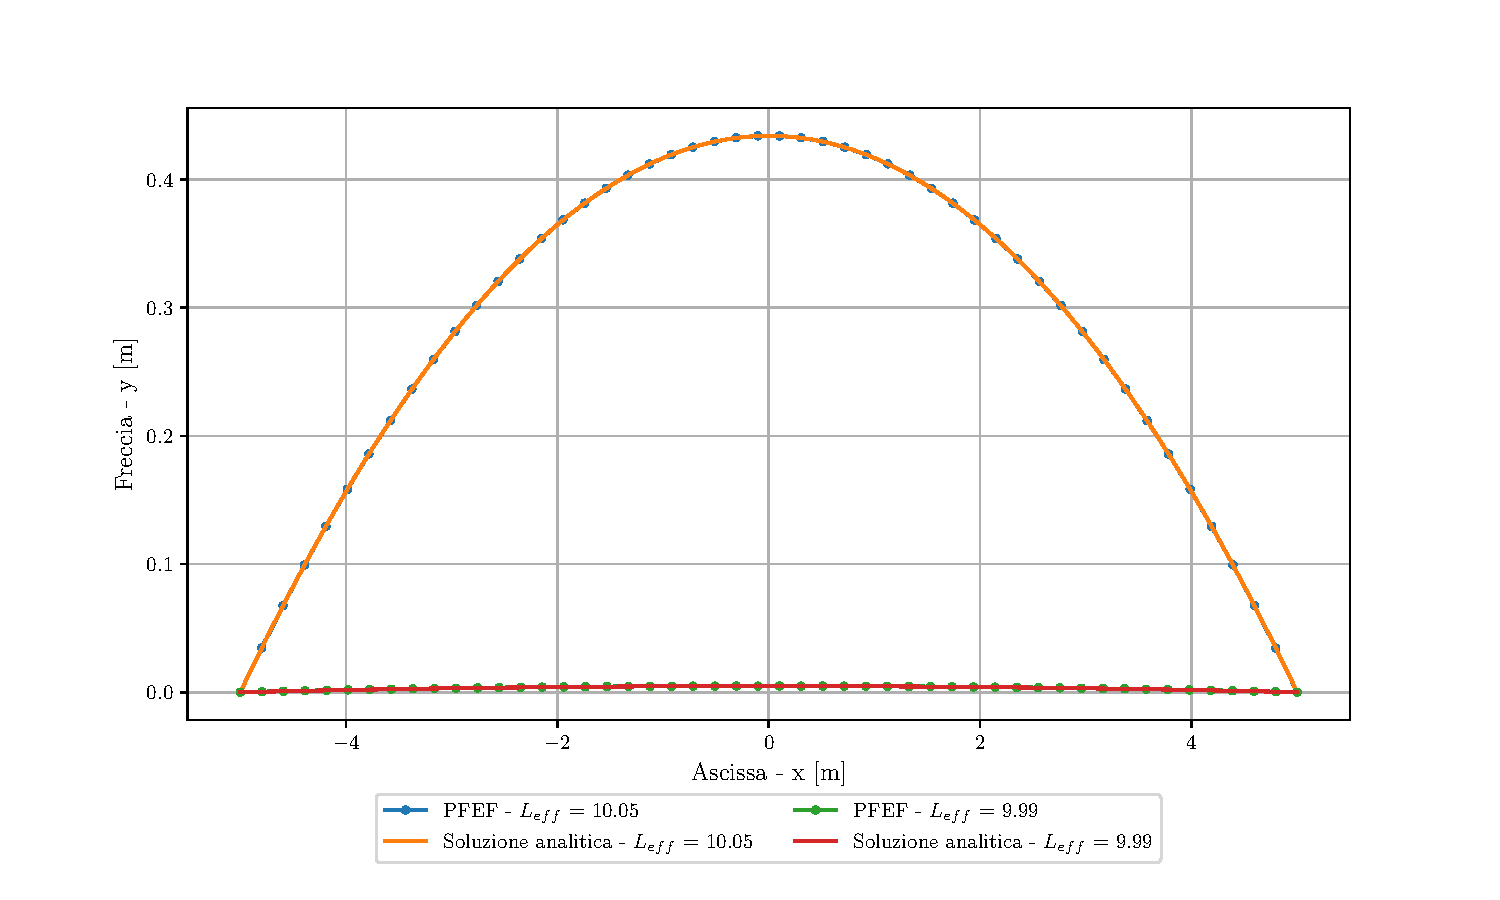
\includegraphics[width=\textwidth]{143_capitoli/capitolo2/immagini_capitolo_2/funePFEF1.pdf}
    \caption{Deformate di funi lasche e tese: Soluzione analitica vs PFEF (mesh = 50 nodi)}
    \label{fig:deformate_PFEF}
\end{figure}

\begin{figure}[htbp]
    \centering
    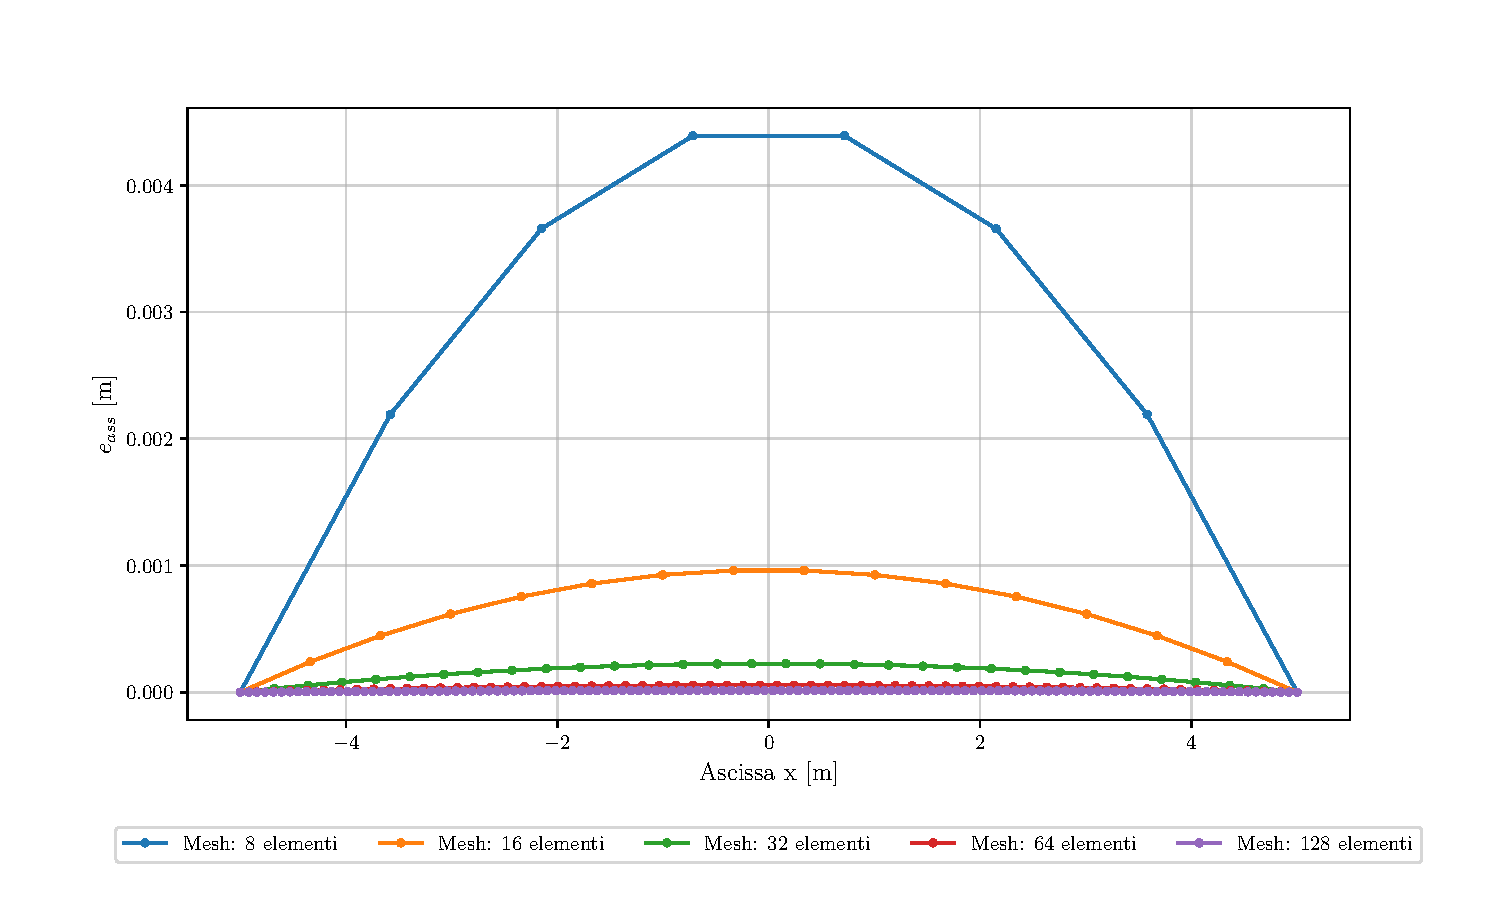
\includegraphics[width=\textwidth]{143_capitoli/capitolo2/immagini_capitolo_2/funePFEF2.pdf}
    \caption{Errore locale sulla deformata - Cavo Lasco ($L_0 = 10.05$)}
    \label{fig:errore_locale1_PFEF}
\end{figure}

\begin{figure}[htbp]
    \centering
    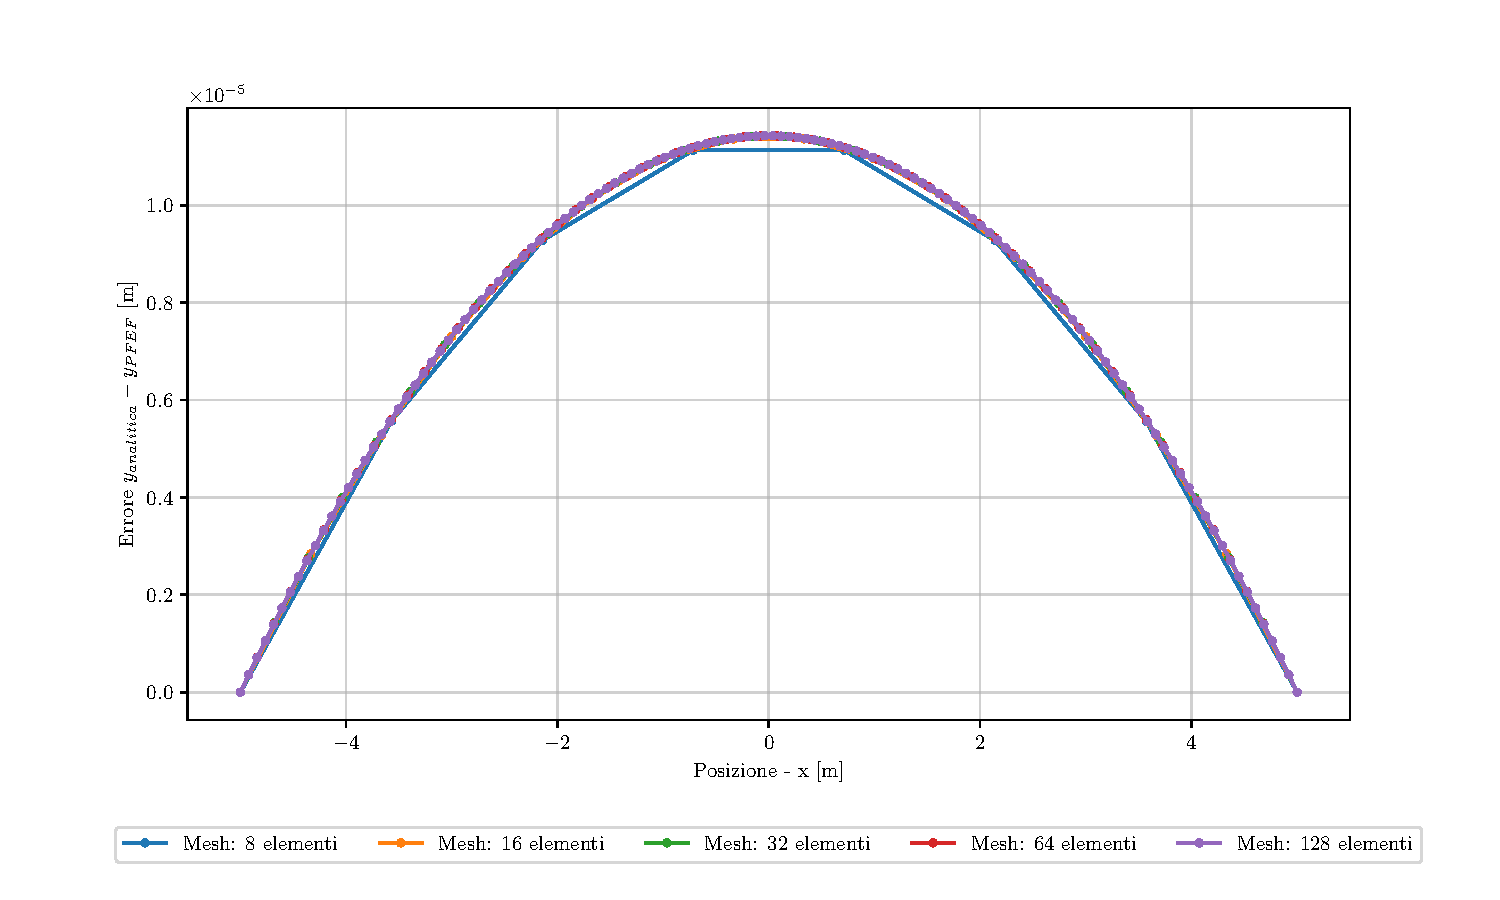
\includegraphics[width=\textwidth]{143_capitoli/capitolo2/immagini_capitolo_2/funePFEF3.pdf}
    \caption{Errore locale sulla deformata - Cavo Teso ($L_0 = 9.99$)}
    \label{fig:errore_locale2_PFEF}
\end{figure}

\begin{figure}[htbp]
    \centering
    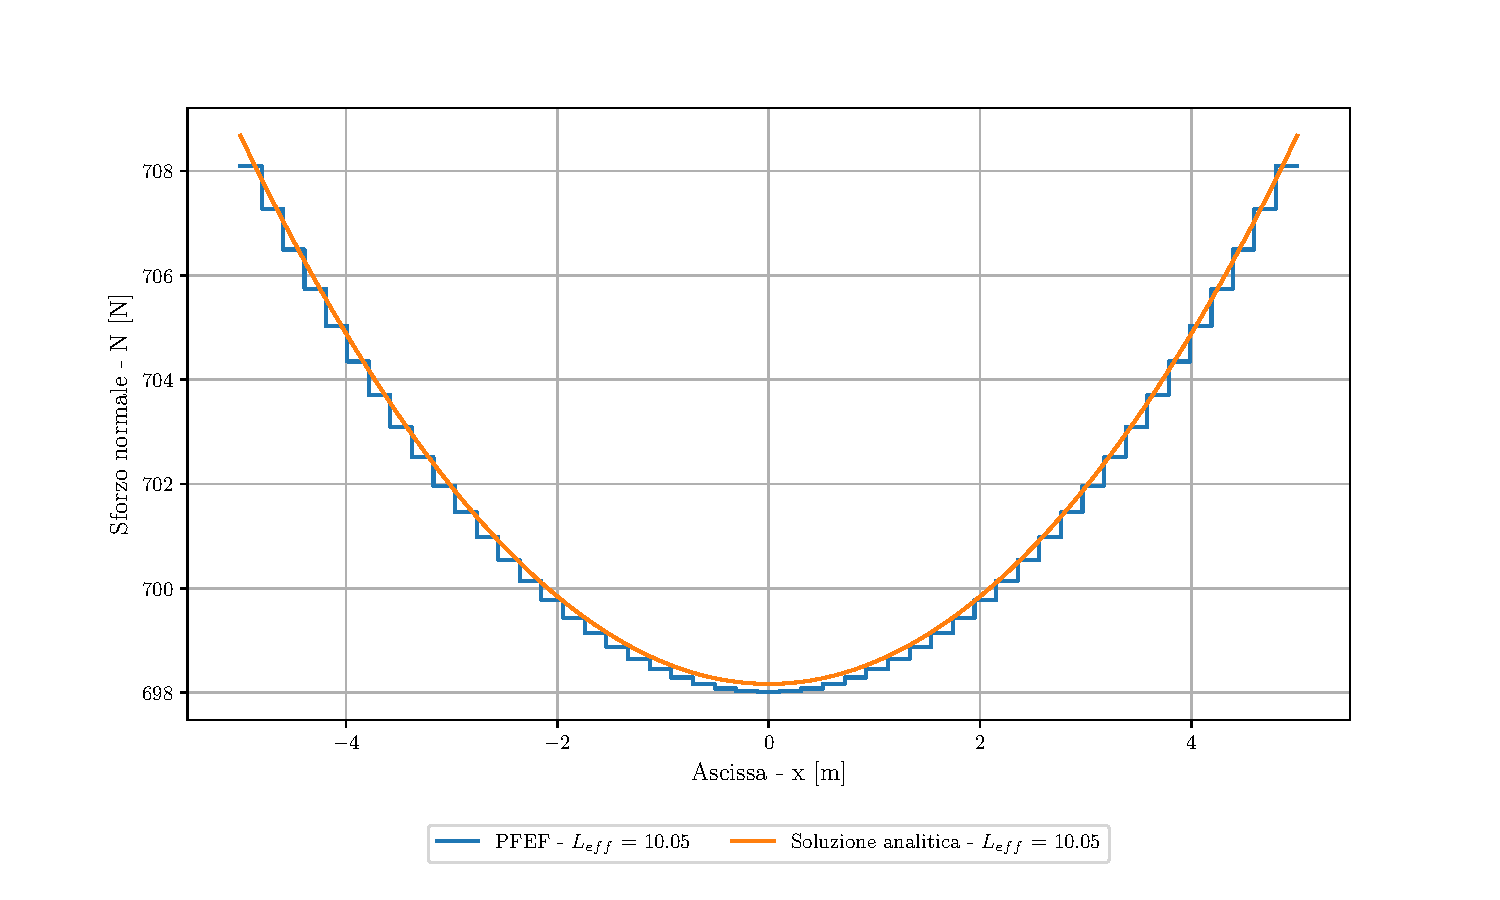
\includegraphics[width=\textwidth]{143_capitoli/capitolo2/immagini_capitolo_2/funePFEF4.pdf}
    \caption{Sforzo normale: Soluzione analitica vs PFEF - Cavo Lasco ($L_0 = 10.05$)}
    \label{fig:sforzonormale1_PFEF}
\end{figure}

\begin{figure}[htbp]
    \centering
    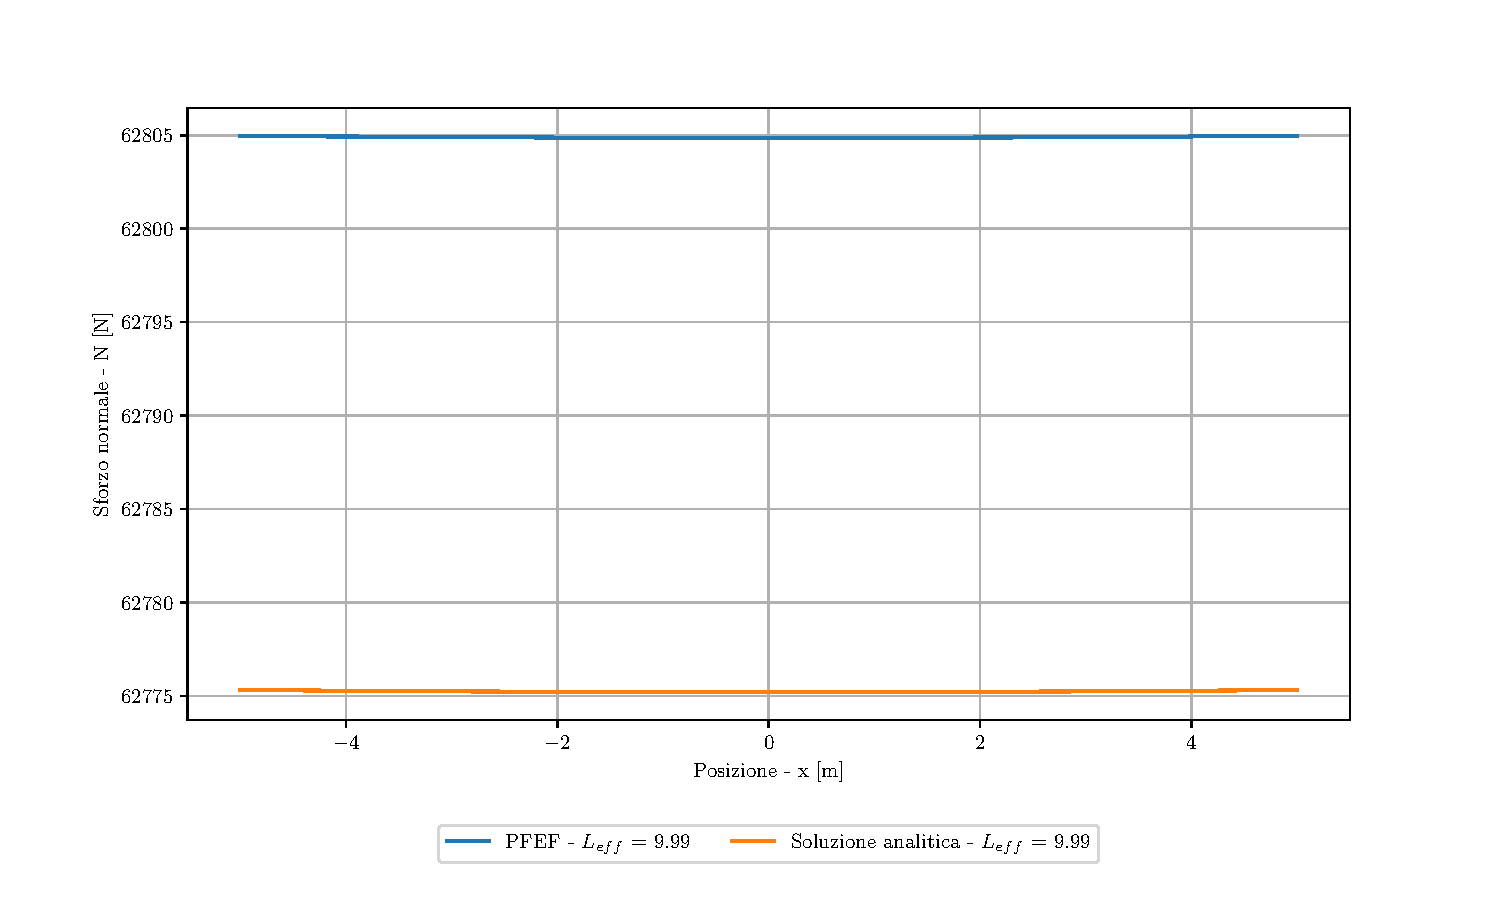
\includegraphics[width=\textwidth]{143_capitoli/capitolo2/immagini_capitolo_2/funePFEF5.pdf}
    \caption{Sforzo normale: Soluzione analitica vs PFEF - Cavo Teso ($L_0 = 9.99$)}
    \label{fig:sforzonormale2_PFEF}
\end{figure}

\section{Reti di funi}
La concordanza appena mostrata tra la soluzione analitica della catenaria e la formulazione numerica PFEF costituisce una fondamentale validazione del codice. Sotto questo profilo, è necessario evidenziare che il problema bidimensionale del singolo cavo e quello tridimensionale di una rete di funi presentano differenze sostanziali nel significato fisico e nello scopo geometrico assegnato alla discretizzazione: 
\begin{itemize}
   \item nel caso bidimensionale: il singolo elemento FEM ha il compito di approssimare la continuità di un unico tratto di fune soggetto a carico distribuito (peso proprio), riproducendone numericamente la curvatura e la distribuizione dello sforzo normale;
   \item nel caso tridimensionale, l'elemento lineare compreso tra due nodi della rete assume invece il ruolo di simulare un segmento di fune tesa, in cui l'effetto del peso proprio del singolo tratto diventa trascurabile rispetto alle forze concentrate scambiate ai nodi. L'elemento assume quindi il significato fisico di un tirante rettilineo. 
\end{itemize}

Nonostante gli scopi strutturali dell'elemento siano differenti nei due scenari, il superamento del test della catenaria bidimensionale rimane un passaggio imprescindibile. Una rete di funi, caratterizzata da una risposta strutturale complessa, è costituita dall'assemblaggio di singoli elementi cavo. Validare accuratamente il singolo elemento rispetto ad un problema continuo bidimensionale garantisce la rigorosità del legame costitutivo, della cinematica non lineare (Green-Lagrange) e dell'algoritmo di Newton-Raphson. Questa robustezza numerica rappresenta il prerequisito necessario per l'estensione del modello ai sistemi di reti tridimensionali e per la successiva implementazione ai problemi di contatto. 

Poichè la formulazione matematica elementare non richiede variazioni nel passaggio al modello tridimensionale, l'obiettivo principale in tale circostanza è stato quello di sviluppare degli strumenti per mezzo dei quali poter valutare una vasta gamma di casistiche reali e rispondere alle principali richieste in campo tecnico come già accenato all'interno del capitolo 1, agendo su alcuni aspetti fondamentali: 
\begin{itemize}
   \item \textbf{Geometria della maglia (\textit{mesh pattern}):} nei sistemi di protezioni regolati dalla norma \cite{EN1263-1}, la geometria della maglia può assumere due pattern distinti: a maglie quadrate (\textit{squared mesh}, contraddistinta dalla lettera Q) o a maglie a forma di diamante (\textit{diamond mesh}, D). L'architettura del codice consente tuttavia la specializzazione verso geometrie arbitrarie in ottica di consentire l'ottimizzazione nell'ambito della progettazione meccanica delle reti; a tal proposito, vengono riportati anche i risultati relativi a reti a base quadrata con elementi fune disposti lungo le diagonali principali. La gestione dell'assemblaggio dei FE avviene per mezzo della matrice di connettività, definita in funzione della geometria scelta, che verrà approfondita nelle sezioni successive. 
   \item \textbf{Vincoli esterni (\textit{supports}):} al fine di riprodurre le reali modalità di serraggio e vincolo applicate ai nodi perimetrali della rete, il comportamento dei supporti è stato idealizzato tramite vincoli cinematici rigidi (come cerniere fisse) o parzialmente cedevoli (come cerniere mobili). Oltre alla natura intrinseca del vincolo, il solutore permette di modificarne la disposizione geometrica lungo il perimetro per mezzo di schemi preconfigurati (ad esempio vincoli differenti a seconda del lato di perimetro che si vuole vincolare), consententendo l'analisi meccanica di reti parzialmente vincolate o sospese esclusivamente in corrispondenza dei vertici. 
   \item \textbf{Disomogeneità meccanica dei cavi:} in conformità con le prescrizioni tecniche della norma \cite{EN1263-1} le reti impiegate possono essere dotate di una fune di bordo (\textit{border rope}). Per riprodurre questa disomogeneità di rigidezza tra le funi di maglia, di bordo e di diagonale, il codice gestisce la variazione delle proprietà meccaniche tramite la modulazione dell'area della sezione trasversale $A$. Tale sezione viene assunta idealmente come circolare e governata analiticamente per mezzo di un raggio fittizio $r$, consentendo così la differenziazione meccanica a livello del singolo elemento fune. La definizione di tali proprietà geometriche avviene nel solutore attraverso configurazioni prestabilite, strutturate per analizzare scenari caratterizzati da rigidezze assiali differenti: elementi a sezione uniforme su tutto il dominio, sezioni differenziate tra maglia interna e funi di bordo, ed infine un modello che distingue tra funi di maglia, di bordo e diagonali strutturali. 
   \item \textbf{Lunghezza dei lati della rete:} un parametro fondamentale per lo svolgimento della prova di assorbimento statico dell'energia da parte di una rete, come specificato in \cite{EN1263-1}, è l'abbassamento iniziale massimo dovuto al solo peso proprio della rete (\textit{sag}), il quale deve attestarsi su un valore pari a $5 \pm 1 cm$. Poichè lo standard normativo prevede che la rete sia posizionata in opera senza l'applicazione di un pretensionamento iniziale, l'unico parametro geometrico che consente di calibrare questa freccia flessionale è il rapporto tra la lunghezza effettiva dei lati della rete a riposo ($L_x$ e $L_y$), e la distanza tra i bordi vincolati ($l_x$ e $l_y$). Come espresso nel Capitolo 1, l'indagine si limita a domini a base rettangolare o quadrata, a seguito della maggior richiesta sul mercato. Il problema computazionale si riduce, pertanto, alla valutazione e alla taratura della tolleranza geometrica da adottare sulle lunghezze dei lati affinchè l'abbassamento ottenuto rientri nel range normativo.    
\end{itemize}

\subsection{Topologia strutturale e matrice di connettività}\label{chap:connettività}
Alla base del Metodo degli Elementi Finiti, ed in modo analogo all'interno della formulazione Position-based qui adottata, il problema meccanico viene governato attraverso le coordinate spaziali di un insieme discreto di nodi, i quali si muovono nello spazio in funzione delle proprietà costitutive e geometriche degli elementi interconnessi. Dal punto di vista topologico, l'insieme di tali nodi, collegati vicendevolmente da elementi lineari, costituisce per definizione un grafo. 

Nel caso specifico delle reti di funi, il sistema può essere descritto associandovi un grafo orientato astratto, la cui struttura spaziale viene mappata ricorrendo all'ordine lessicografico. L'associazione tra la struttura reale discretizzata e la teoria dei grafi consente di sfruttare le proprietà dell'ordinamento lessicografico per gestire, in modo rigoroso e modulare, sia la generazione automatica della matrice di connettività, sia l'individuazione di specifiche famiglie di nodi (come i nodi di bordo, i nodi appartenenti alle diagonali principali o i vertici d'angolo) all'interno dello spazio computazionale.

L'ordine lessicografico è un criterio di ordinamento di una sequenza di simboli per cui è già presente un ordine interno. Date due famiglie di insiemi ordinati, come quelle che contengono la numerazione di righe $J = \{j_0, j_1, \dots , j_m\}$ e colonne $I = \{i_0, i_1, \dots, i_n\}$ della griglia in cui è suddiviso il dominio della rete, è possibile applicare l'ordinamento lessicografico sulle coppie di valori di righe e colonne $(i,j)$ per mapparle in un indice lineare coerente attraverso la formula: 
\begin{equation}
     N = j \cdot n_x + i 
\end{equation}  
dove: 
\begin{itemize}
   \item $N$ è l'indice lineare univoco associato al generico nodo;
   \item $n_x$ è il numero totale di nodi presenti su ciascuna riga, pari a $n_x = n + 1$;
   \item $j \in J$ è l'indice di riga relativo al nodo indicato ($j = 0, 1, \dots, m$)
   \item $i \in I$ è l'indice di colonna relativo al nodo indicato ($i = 0, 1, \dots, n$)
\end{itemize}

\begin{figure}[htbp]
    \centering
    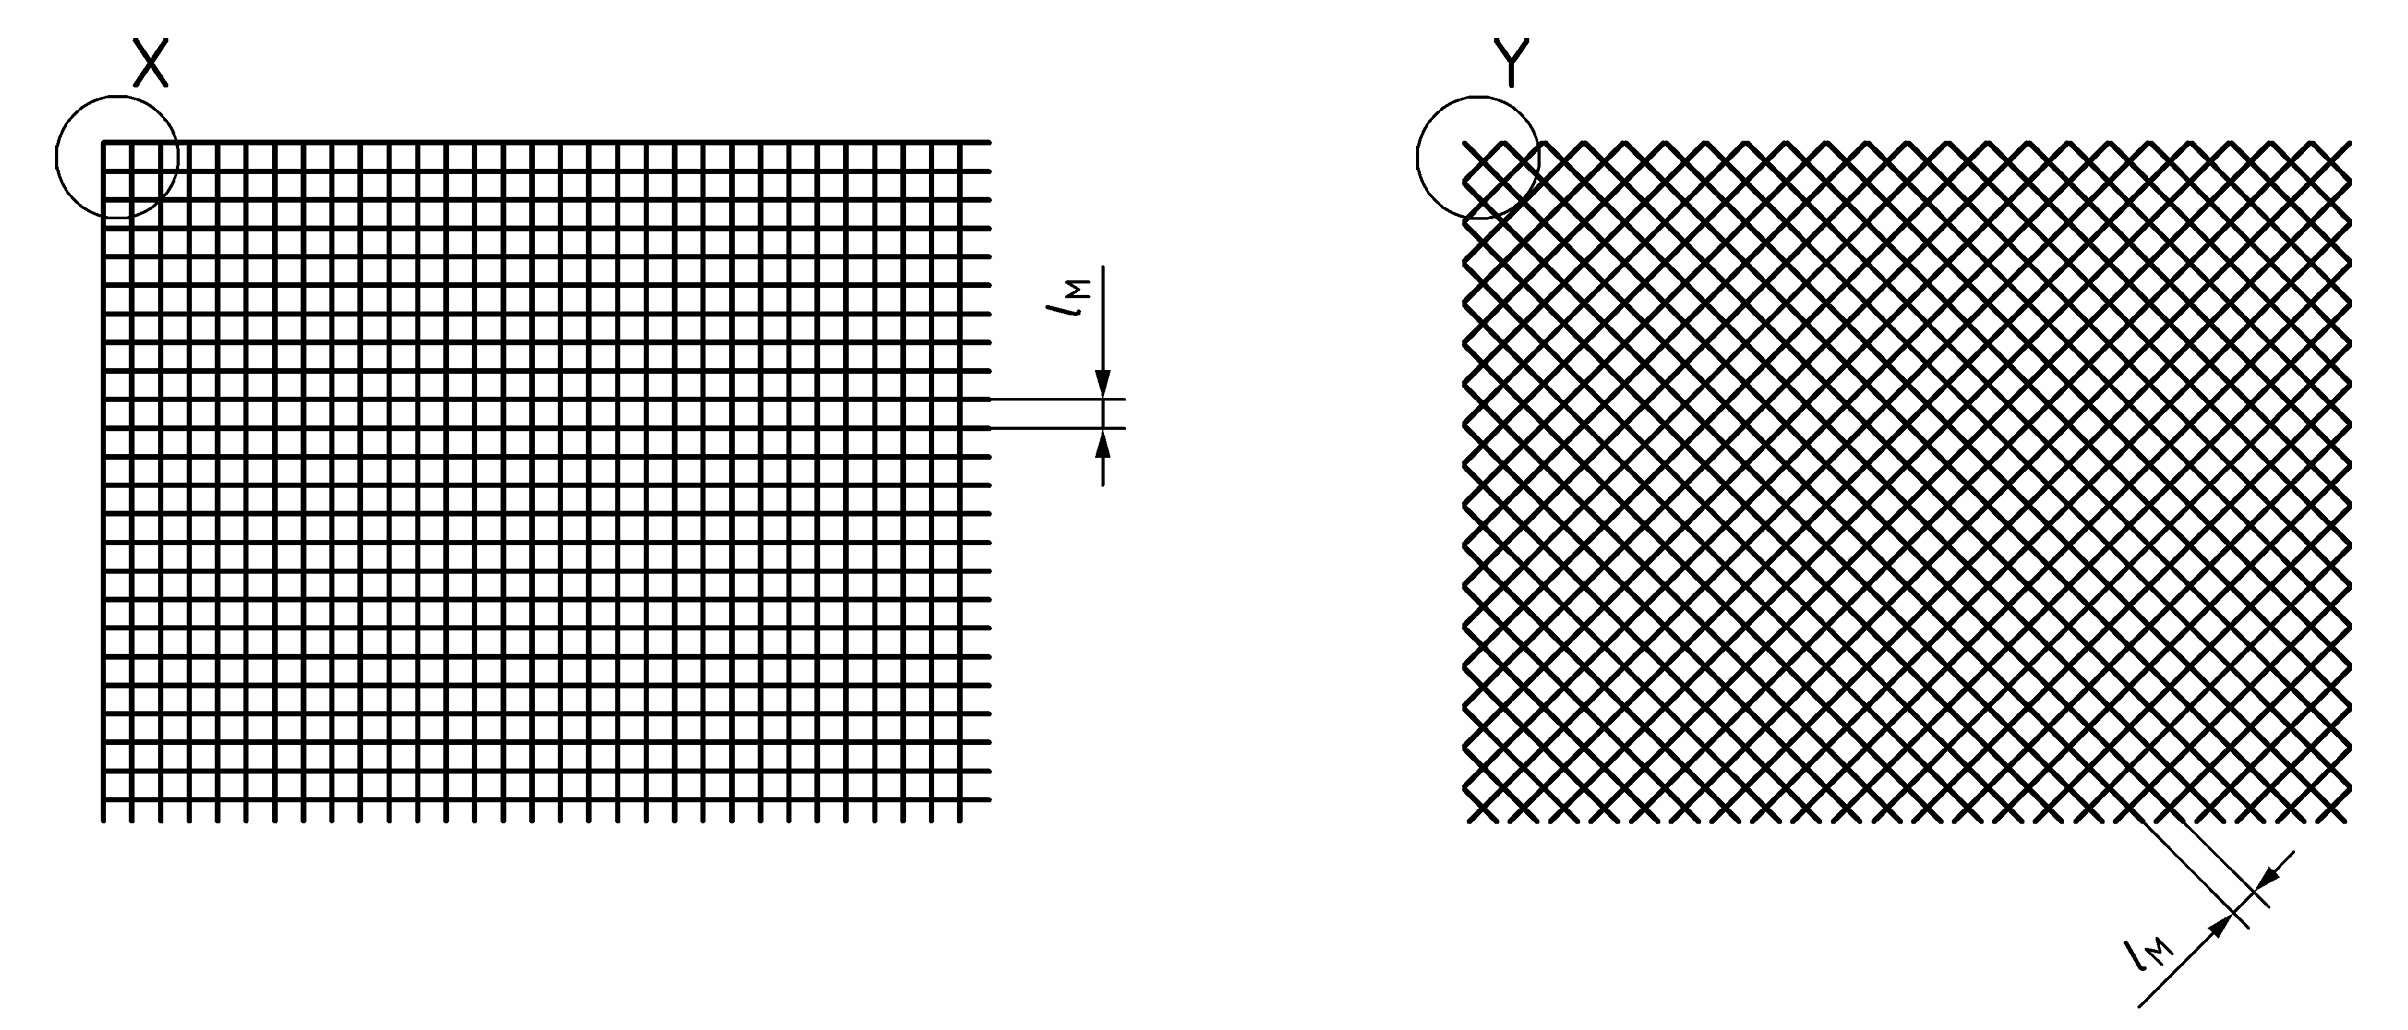
\includegraphics[width=\textwidth]{143_capitoli/capitolo2/immagini_capitolo_2/mesh_pattern.png}
    \caption{Mesh pattern normati: 'X' squared mesh (Q) - 'Y' diamond mesh (D)}
    \label{fig:pattern_mesh}
\end{figure}


A titolo esemplificativo, consideriamo le mesh pattern standard $Q$ e $D$ previste dalla norma \cite{EN1263-1} e riportate in \cref{fig:pattern_mesh}. Per entrambe le configurazioni, l'ordinamento lessicografico definisce la sequenza con cui avviene la numerazione dei nodi della maglia, sebbene venga declinato secondo logiche di scansione differenti: 
\begin{itemize}
   \item nel caso di \textit{squared mesh} (Q), l'ordine lessicografico segue una scansione cartesiana standard per righe e colonne parallele agli assi principali del dominio di posa della rete. In questa configurazione, ogni intersezione della griglia corrisponde univocamente a un nodo strutturale e ad un incrocio di filamenti ortogonali, come rappresentato nel grafo di \cref{fig:grafo_squared};
   \item nel caso di \textit{diamond mesh} (D), l'ordinamento definisce la medesima disposizione spaziale dei nodi, ma la matrice di connettività viene modificata per mappare l'orientamento inclinato a rombo dei singoli elementi fune. Al fine di descrivere la caratteristica alternanza geometrica a scacchiera senza altere la mappatura dei nodi, la procedura attraverso cui viene compilata la matrice di connettività opera distinguendo la parità della somma degli indici di riga e colonna $(i + j)$. Gli elementi interni vengono così tesi lungo le diagonali geoemetriche dei quadrati logici, mentra gli elementi perimetrali di bordo vengono generati campionando i nodi con passo doppio, garantendo la perfetta chiusura dei triangoli esterni (vedi \cref{fig:grafo_diamond}).
\end{itemize}

\begin{figure}[htbp]
    \centering
    % Contenuto di "143_capitoli/capitolo2/immagini_capitolo_2/grafo_squared.tex"
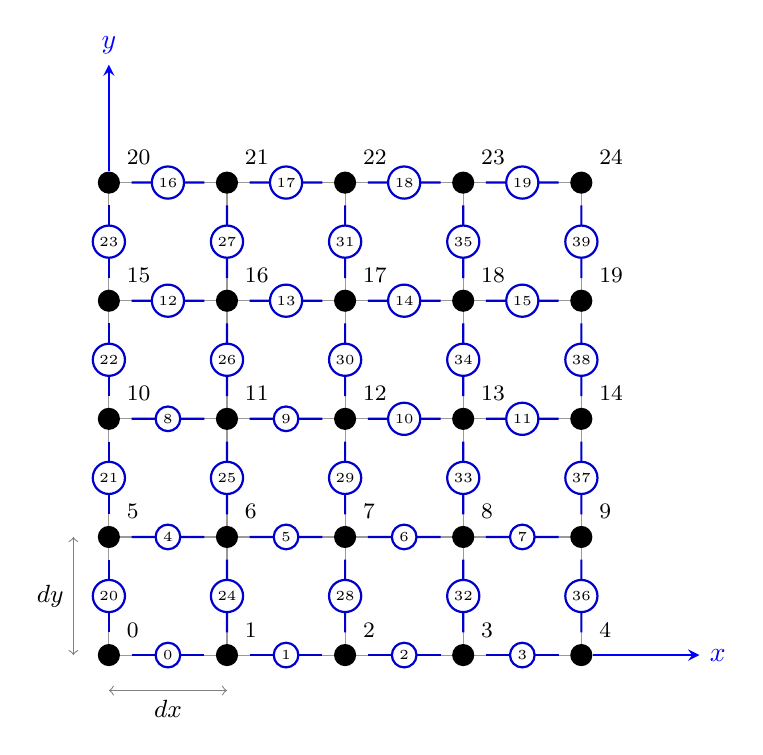
\begin{tikzpicture}[
    scale=1.5, 
    punto/.style={circle, fill=black, inner sep=0pt, minimum size=8pt}, 
    fune/.style={draw=blue!80!black, thick, shorten >=4pt, shorten <=4pt}, 
    asse/.style={->, >=stealth, blue, thick},
    el_oriz/.style={circle, draw=blue!80!black, fill=white, font=\tiny\color{black}, inner sep=1.5pt},
    el_vert/.style={circle, draw=blue!80!black, fill=white, font=\tiny\color{black}, inner sep=1.5pt},
    every label/.style={font=\footnotesize, black} 
]

    % 1. Assi cartesiani
    \draw[asse] (4.1,0) -- (5.0,0) node[right] {$x$};
    \draw[asse] (0,4.1) -- (0, 5.0) node[above] {$y$};
    
    % LA GRIGLIA DI SFONDO
    % Disegna una griglia dal punto (0,0) al punto (4,4) con passo 1.0 (coincidente con i nodi)
    \draw[gray!80, thin, step = 1.0] (0,0) grid (4,4);
    
    % Quote passi dx e dy
    \draw[<->, gray] (0,-0.3) -- (1,-0.3) node[midway, below, black] {\small $dx$};
    \draw[<->, gray] (-0.3,0) -- (-0.3,1) node[midway, left, black] {\small $dy$};

    % 2. Definizione dei Nodi (25 nodi totali, matrice 5x5, nx = 5)
    % Riga y = 0
    \node[punto, label={45:0}] (N0) at (0,0) {};
    \node[punto, label={45:1}] (N1) at (1,0) {};
    \node[punto, label={45:2}] (N2) at (2,0) {};
    \node[punto, label={45:3}] (N3) at (3,0) {};
    \node[punto, label={45:4}] (N4) at (4,0) {};
    
    % Riga y = 1
    \node[punto, label={45:5}] (N5) at (0,1) {};
    \node[punto, label={45:6}] (N6) at (1,1) {};
    \node[punto, label={45:7}] (N7) at (2,1) {};
    \node[punto, label={45:8}] (N8) at (3,1) {};
    \node[punto, label={45:9}] (N9) at (4,1) {};
    
    % Riga y = 2
    \node[punto, label={45:10}] (N10) at (0,2) {};
    \node[punto, label={45:11}] (N11) at (1,2) {};
    \node[punto, label={45:12}] (N12) at (2,2) {};
    \node[punto, label={45:13}] (N13) at (3,2) {};
    \node[punto, label={45:14}] (N14) at (4,2) {};
    
    % Riga y = 3
    \node[punto, label={45:15}] (N15) at (0,3) {};
    \node[punto, label={45:16}] (N16) at (1,3) {};
    \node[punto, label={45:17}] (N17) at (2,3) {};
    \node[punto, label={45:18}] (N18) at (3,3) {};
    \node[punto, label={45:19}] (N19) at (4,3) {};
    
    % Riga y = 4
    \node[punto, label={45:20}] (N20) at (0,4) {};
    \node[punto, label={45:21}] (N21) at (1,4) {};
    \node[punto, label={45:22}] (N22) at (2,4) {};
    \node[punto, label={45:23}] (N23) at (3,4) {};
    \node[punto, label={45:24}] (N24) at (4,4) {};

    % 3. Elementi Orizzontali (20 elementi, numeri da 0 a 19 cerchiati sulla fune)
    % y = 0
    \draw[fune] (N0) -- (N1) node[midway, el_oriz] {0};
    \draw[fune] (N1) -- (N2) node[midway, el_oriz] {1};
    \draw[fune] (N2) -- (N3) node[midway, el_oriz] {2};
    \draw[fune] (N3) -- (N4) node[midway, el_oriz] {3};
    
    % y = 1
    \draw[fune] (N5) -- (N6) node[midway, el_oriz] {4};
    \draw[fune] (N6) -- (N7) node[midway, el_oriz] {5};
    \draw[fune] (N7) -- (N8) node[midway, el_oriz] {6};
    \draw[fune] (N8) -- (N9) node[midway, el_oriz] {7};
    
    % y = 2
    \draw[fune] (N10) -- (N11) node[midway, el_oriz] {8};
    \draw[fune] (N11) -- (N12) node[midway, el_oriz] {9};
    \draw[fune] (N12) -- (N13) node[midway, el_oriz] {10};
    \draw[fune] (N13) -- (N14) node[midway, el_oriz] {11};
    
    % y = 3
    \draw[fune] (N15) -- (N16) node[midway, el_oriz] {12};
    \draw[fune] (N16) -- (N17) node[midway, el_oriz] {13};
    \draw[fune] (N17) -- (N18) node[midway, el_oriz] {14};
    \draw[fune] (N18) -- (N19) node[midway, el_oriz] {15};
    
    % y = 4
    \draw[fune] (N20) -- (N21) node[midway, el_oriz] {16};
    \draw[fune] (N21) -- (N22) node[midway, el_oriz] {17};
    \draw[fune] (N22) -- (N23) node[midway, el_oriz] {18};
    \draw[fune] (N23) -- (N24) node[midway, el_oriz] {19};

    % 4. Elementi Verticali (20 elementi, numeri da 20 a 39 cerchiati sulla fune)
    % x = 0
    \draw[fune] (N0) -- (N5) node[midway, el_vert] {20};
    \draw[fune] (N5) -- (N10) node[midway, el_vert] {21};
    \draw[fune] (N10) -- (N15) node[midway, el_vert] {22};
    \draw[fune] (N15) -- (N20) node[midway, el_vert] {23};
    
    % x = 1
    \draw[fune] (N1) -- (N6) node[midway, el_vert] {24};
    \draw[fune] (N6) -- (N11) node[midway, el_vert] {25};
    \draw[fune] (N11) -- (N16) node[midway, el_vert] {26};
    \draw[fune] (N16) -- (N21) node[midway, el_vert] {27};
    
    % x = 2
    \draw[fune] (N2) -- (N7) node[midway, el_vert] {28};
    \draw[fune] (N7) -- (N12) node[midway, el_vert] {29};
    \draw[fune] (N12) -- (N17) node[midway, el_vert] {30};
    \draw[fune] (N17) -- (N22) node[midway, el_vert] {31};
    
    % x = 3
    \draw[fune] (N3) -- (N8) node[midway, el_vert] {32};
    \draw[fune] (N8) -- (N13) node[midway, el_vert] {33};
    \draw[fune] (N13) -- (N18) node[midway, el_vert] {34};
    \draw[fune] (N18) -- (N23) node[midway, el_vert] {35};
    
    % x = 4
    \draw[fune] (N4) -- (N9) node[midway, el_vert] {36};
    \draw[fune] (N9) -- (N14) node[midway, el_vert] {37};
    \draw[fune] (N14) -- (N19) node[midway, el_vert] {38};
    \draw[fune] (N19) -- (N24) node[midway, el_vert] {39};

\end{tikzpicture}
    \caption{Rappresentazione topologica della \textit{squared mesh} (Q) tramite grafo orientato: numerazione dei nodi secondo l'ordine lessicografico cartesiano e orientamento locale degli elementi fune.}
    \label{fig:grafo_squared}
\end{figure}

\begin{figure}[htbp]
    \centering
    % Contenuto di "143_capitoli/capitolo2/immagini_capitolo_2/grafo_diamond.tex"
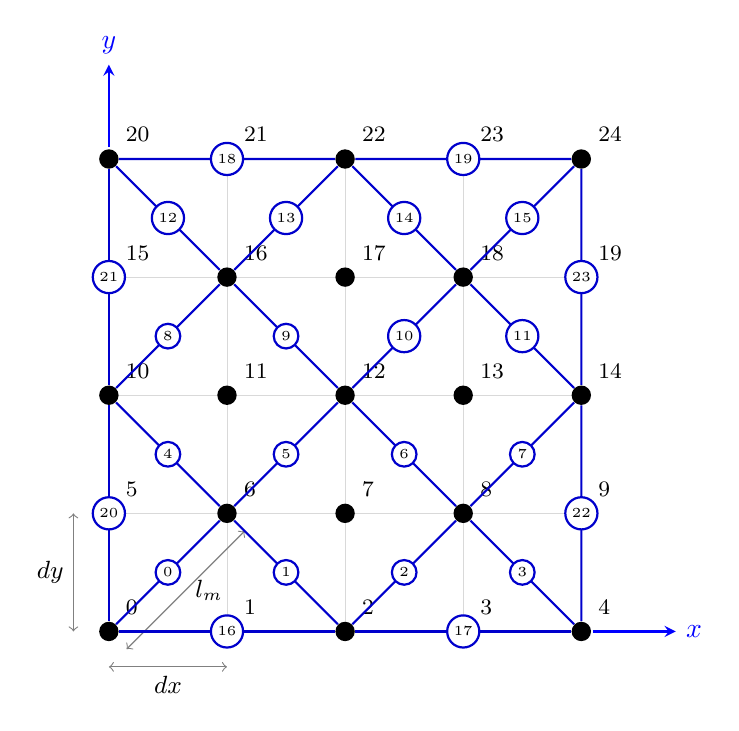
\begin{tikzpicture}[
    scale=1.5, 
    punto/.style={circle, fill=black, inner sep=0pt, minimum size=7pt}, 
    fune/.style={draw=blue!80!black, thick, shorten >=0pt, shorten <=0pt}, 
    asse/.style={->, >=stealth, blue, thick},
    el/.style={circle, draw=blue!80!black, fill=white, font=\tiny, inner sep=1.5pt},
    every label/.style={font=\footnotesize, text=black} 
]

    % 1. Assi cartesiani
    \draw[asse] (4.1,0) -- (4.8,0) node[right] {$x$};
    \draw[asse] (0,4.1) -- (0, 4.8) node[above] {$y$};
    
    % Griglia di sfondo fissa (passo 0.5)
    \draw[gray!30, very thin, step=1] (0,0) grid (4,4);
    
    % Quote passi dx, dy (valgono 1.0 geometrico per n=4, m=4)
    \draw[<->, gray] (0,-0.3) -- (1,-0.3) node[midway, below, black] {\small $dx$};
    \draw[<->, gray] (-0.3,0) -- (-0.3,1) node[midway, left, black] {\small $dy$};
    % Quota della maglia diagonale lm
    \draw[<->, gray] (0.15,-0.15) -- (1.15,0.85) node[midway, right, black] {\small $l_m$};

    % 2. Generazione dei 25 Nodi (Matrice 5x5, da 0 a 24, nx = 5)
    % y = 0
    \node[punto, label={45:0}]  (N0)  at (0,0) {};
    \node[punto, label={45:1}]  (N1)  at (1,0) {};
    \node[punto, label={45:2}]  (N2)  at (2,0) {};
    \node[punto, label={45:3}]  (N3)  at (3,0) {};
    \node[punto, label={45:4}]  (N4)  at (4,0) {};
    % y = 1
    \node[punto, label={45:5}]  (N5)  at (0,1) {};
    \node[punto, label={45:6}]  (N6)  at (1,1) {};
    \node[punto, label={45:7}]  (N7)  at (2,1) {};
    \node[punto, label={45:8}]  (N8)  at (3,1) {};
    \node[punto, label={45:9}]  (N9)  at (4,1) {};
    % y = 2
    \node[punto, label={45:10}] (N10) at (0,2) {};
    \node[punto, label={45:11}] (N11) at (1,2) {};
    \node[punto, label={45:12}] (N12) at (2,2) {};
    \node[punto, label={45:13}] (N13) at (3,2) {};
    \node[punto, label={45:14}] (N14) at (4,2) {};
    % y = 3
    \node[punto, label={45:15}] (N15) at (0,3) {};
    \node[punto, label={45:16}] (N16) at (1,3) {};
    \node[punto, label={45:17}] (N17) at (2,3) {};
    \node[punto, label={45:18}] (N18) at (3,3) {};
    \node[punto, label={45:19}] (N19) at (4,3) {};
    % y = 4
    \node[punto, label={45:20}] (N20) at (0,4) {};
    \node[punto, label={45:21}] (N21) at (1,4) {};
    \node[punto, label={45:22}] (N22) at (2,4) {};
    \node[punto, label={45:23}] (N23) at (3,4) {};
    \node[punto, label={45:24}] (N24) at (4,4) {};

    % 3. ELEMENTI INTERNI (16 Diagonali alternate dall'output per n=4, m=4)
    % j = 0
    \draw[fune] (N0)  -- (N6)  node[midway, el] {0};   % (0+0)%2 == 0 -> SW-NE
    \draw[fune] (N2)   -- (N6)  node[midway, el] {1};   % (1+0)%2 != 0 -> SE-NW
    \draw[fune] (N2)  -- (N8)  node[midway, el] {2};   % (2+0)%2 == 0 -> SW-NE
    \draw[fune] (N4)   -- (N8)  node[midway, el] {3};   % (3+0)%2 != 0 -> SE-NW
    
    % j = 1
    \draw[fune] (N10) -- (N6)  node[midway, el] {4};   % (0+1)%2 != 0 -> SE-NW
    \draw[fune] (N6)  -- (N12) node[midway, el] {5};   % (1+1)%2 == 0 -> SW-NE
    \draw[fune] (N12) -- (N8)  node[midway, el] {6};   % (2+1)%2 != 0 -> SE-NW
    \draw[fune] (N8)  -- (N14) node[midway, el] {7};   % (3+1)%2 == 0 -> SW-NE
    
    % j = 2
    \draw[fune] (N10) -- (N16) node[midway, el] {8};   % (0+2)%2 == 0 -> SW-NE
    \draw[fune] (N12) -- (N16) node[midway, el] {9};   % (1+2)%2 != 0 -> SE-NW
    \draw[fune] (N12) -- (N18) node[midway, el] {10};  % (2+2)%2 == 0 -> SW-NE
    \draw[fune] (N14) -- (N18) node[midway, el] {11};  % (3+2)%2 != 0 -> SE-NW
    
    % j = 3
    \draw[fune] (N20) -- (N16) node[midway, el] {12};  % (0+3)%2 != 0 -> SE-NW
    \draw[fune] (N16) -- (N22) node[midway, el] {13};  % (1+3)%2 == 0 -> SW-NE
    \draw[fune] (N22) -- (N18) node[midway, el] {14};  % (2+3)%2 != 0 -> SE-NW
    \draw[fune] (N18) -- (N24) node[midway, el] {15};  % (3+3)%2 == 0 -> SW-NE

    % 4. ELEMENTI DI BORDO (8 Elementi perimetrali a passo 2)
    % Bordo x in basso
    \draw[fune] (N0)  -- (N2)  node[midway, el] {16};
    \draw[fune] (N2)  -- (N4)  node[midway, el] {17};
    
    % Bordo x in alto
    \draw[fune] (N20) -- (N22) node[midway, el] {18};
    \draw[fune] (N22) -- (N24) node[midway, el] {19};
    
    % Bordo sinistro y
    \draw[fune] (N0)  -- (N10) node[midway, el] {20};
    \draw[fune] (N10) -- (N20) node[midway, el] {21};
    
    % Bordo destro y
    \draw[fune] (N4)  -- (N14) node[midway, el] {22};
    \draw[fune] (N14) -- (N24) node[midway, el] {23};

\end{tikzpicture}
    \caption{Rappresentazione topologica della \textit{Diamond mesh} (D) tramite grafo orientato: numerazione dei nodi secondo l'ordine lessicografico cartesiano e orientamento locale degli elementi fune.}
    \label{fig:grafo_diamond}
\end{figure}

\vspace{1em}
\subsubsection{Matrice di connettività}
La matrice di connettività è una matrice di dimensioni $n_{elements} \times 2$ che contiene le informazioni topologiche del grafo associato alla struttura di funi. Ciascuna riga $e$ della matrice descrive un elemento d'asta (arco del grafo) e contiene gli indici lineari dei due nodi estremanti ($N_1$, $N_2$) da esso connessi. 

\vspace{1em}
Nel caso di maglia quadrata (\textit{squared mesh (Q)}), la matrice di connettività è generata coerentemente con la numerezione riportata in \cref{fig:grafo_squared}. L'algoritmo esegue dapprima un ciclo sulle righe del grafo, perciò le prime $n \times m_y$ righe memorizzano le connessioni orizzontali con indici dei nodi estremi definiti da:
\begin{equation}
   (N_1, N_2) = \bigl(j \cdot n_x + i, \; j \cdot n_x + (i + 1)\bigr)
\end{equation}
successivamente, la scansione procede lungo le colonne, determinando le restanti $m \times n_x$ righe della matrice relative alle connessioni veritcali, i cui indici nodali assumono la forma:
\begin{equation}
   (N_1, N_2) = \bigl(j \cdot n_x + i, \; (j+1) \cdot n_x + i\bigr)
\end{equation}

\vspace{1em}
Nel caso della diamond mesh (\textit{diamond mesh (D)}) la matrice di connettività è costruita coerentemente con l'ordinamento logico illustrato in \cref{fig:grafo_diamond}. In questa configurazione le prime $n \cdot m$  righe contengono informazioni topologiche riguardo agli elementi interni di maglia, mentre le restanti descrivono la connettività tra i nodi di bordo del dominio. 

Mentre per la definizione degli elementi di bordo si applica una logica analoga a quella descritta per la maglia quadrata, la generazione degli elementi interni richiede la formulazione di un algoritmo specifico. Iterando su ciascuna riga della griglia, la connettività dei singoli elementi è governata dalla parità della coordinata discreta del nodo:
\begin{itemize}
    \item Se la somma degli indici di posizione $(i + j)$ risulta \textbf{pari}, l'elemento identifica una diagonale orientata a sinistra; i nodi estremanti associati all'arco sono pertanto identificati dalla relazione:
    \begin{equation}
        (N_1, N_2) = \bigl(j \cdot n_x + i, \; (j + 1) \cdot n_x + (i + 1)\bigr)
    \end{equation}
    \item Se la somma $(i + j)$ risulta \textbf{dispari}, l'elemento individua una diagonale orientata a destra, le cui connessioni nodali sono espresse da:
    \begin{equation}
        (N_1, N_2) = \bigl((j + 1) \cdot n_x + i, \; j \cdot n_x + (i + 1)\bigr)
    \end{equation}
\end{itemize}
Si evidenzia, infine, come la medesima logica di binarizzazione geometrica basata sull'orientamento delle diagonali destre e sinistre trovi applicazione diretta anche per l'identificazione e la mappatura degli elementi controventati nel caso di maglie quadrate con diagonali aggiuntive.

\subsection{Vincoli esterni}
Le reti di sicurezza conformi alla normativa \cite{EN1263-1} possono essere soggette a molteplici configurazioni di vincolamento esterno. Al fine di poter ripordurre fedelmente tali condizioni all'interno del modello, si rende necessaria una formulazione cinematica versatile che consenta di accoppiare i nodi di bordo della rete con l'ambiente circostante, tenendo conto dei reali gradi di libertà concessi dai sistemi di ancoraggio.

All'interno del solutore sviluppato, le condizioni di vincolo esterne applicabili ai singoli nodi computazionali si basano su due modelli cinematici fondamentali, rappresentati in \cref{fig:confronto_vincoli}.
\begin{itemize}
   \item Cerniera fissa (\cref{fig:confronto_vincoli} (a)): blocca tutti i gradi di libertà traslazionali del nodo ($u_{x_1} = 0, u_{x_2} = 0, u_{x_3} = 0$)
   \item Cerniera mobile (\cref{fig:confronto_vincoli} (b)): l'unico grado di libertà del nodo garantisce la traslazione lungo la direzione dell'asse orizziontale su cui esso giace (es. direzione locale $x_j$), consentendogli lo scorrimento cinematico lungo la guida e bloccando i restanti gradi di libertà ortogonali.
\end{itemize}

\begin{figure}[htbp]
    \centering
    % Contenuto di "143_capitoli/capitolo2/immagini_capitolo_2/confronto_vincoli_3d.tex"
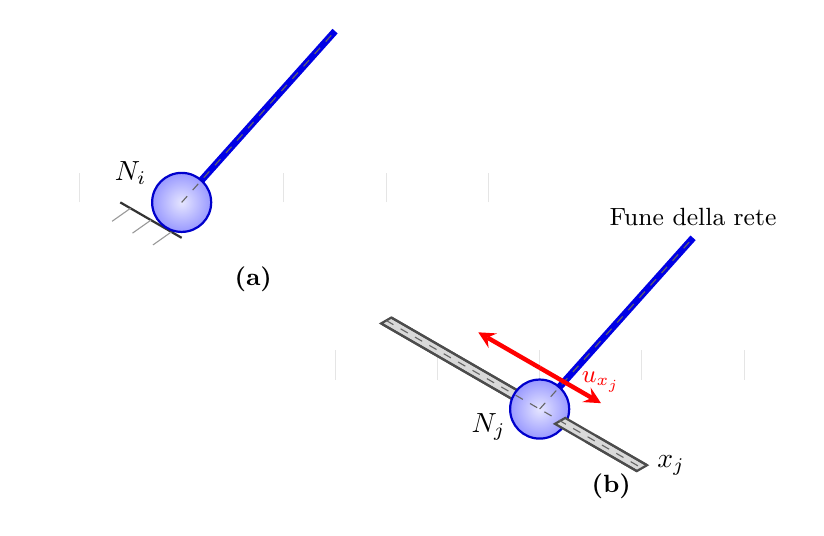
\begin{tikzpicture}[
    scale=1.5,
    x={(0.866cm,-0.5cm)}, y={(0.866cm,0.5cm)}, z={(0cm,1cm)},   % Assonometria isometrica
    guida/.style={draw=black!70, fill=gray!30, thick},
    fune/.style={draw=blue!90!black, line width=2.5pt},
    vettore/.style={->, >=stealth, red, ultra thick},
    titolo/.style={font=\small\bfseries, text=black, align=center}
]

    % =========================================================================
    % 1. SINISTRA: CERNIERA FISSA (Ancorata a terra)
    % =========================================================================
    
    % Piano di fondo locale
    \draw[gray!20, thin, step=0.5] (-1,-0.5,0) grid (1.5,1.5,0);
    
    % Piastra fissa di base a terra (Ancoraggio meccanico strutturale)
    \draw[black!80, thick] (-0.3,-0.3,0) -- (0.3,-0.3,0);
    \foreach \x in {-0.2,0,0.2} {
        \draw[black!40, thin] (\x,-0.3,0) -- (\x-0.08,-0.4,-0.1);
    }

    % Disegno della Fune (prima della sferetta per corretta sovrapposizione)
    \draw[fune] (0,0,0) -- (0.5, 1.0, 1.2);

    % Sferetta del nodo fisso (copre l'inizio della fune)
    \shadedraw[inner color=blue!10, outer color=blue!40, draw=blue!80!black, thick] (0,0,0) circle [radius=0.25cm];

    % Asse della fune (nero tratteggiato, sovrapposto sopra)
    \draw[dashed, black!60, thin] (0,0,0) -- (0.5, 1.0, 1.2);

    % Etichetta del nodo
    \node[black] at (-0.1, -0.4, 0.4) {$N_i$};
    
    % Titolo della subfigura a) bloccato alla quota y=0.5, z=-0.8
    \node[titolo] at (0.2, 0.5, -0.8) {(a)};


    % =========================================================================
    % 2. DESTRA: CERNIERA MOBILE (Su Guida Lineare)
    % =========================================================================
    % Lo shift ora è (3.5, 0, 0) puro: y=0 e z=0 sono identici al precedente.
    % Questo rende le due cerniere perfettamente parallele e complanari.
    \begin{scope}[shift={(3.5,0,0)}]
        
        % Piano di fondo locale
        \draw[gray!20, thin, step=0.5] (-1.5,-0.5,0) grid (1,1.5,0);

        % Guida cilindrica (asse x locale) - parte posteriore
        \fill[guida] (-1.5,-0.05,0) -- (0,-0.05,0) -- (0,0.05,0) -- (-1.5,0.05,0) -- cycle;
        \draw[black!70, thick] (-1.5,-0.05,0) -- (0,-0.05,0);
        \draw[black!70, thick] (-1.5,0.05,0) -- (0,0.05,0);

        % Disegno della Fune
        \draw[fune] (0,0,0) -- (0.5, 1.0, 1.2) node[above, black] {\small Fune della rete};

        % Sferetta del nodo mobile (copre l'inizio della fune e la parte posteriore della guida)
        \shadedraw[inner color=blue!10, outer color=blue!40, draw=blue!80!black, thick] (0,0,0) circle [radius=0.25cm];

        % Parte anteriore della guida
        \fill[guida] (0.2,-0.05,0) -- (1.0,-0.05,0) -- (1.0,0.05,0) -- (0.2,0.05,0) -- cycle;
        \draw[black!70, thick] (0.5,-0.05,0) -- (1.0,-0.05,0);
        \draw[black!70, thick] (0.5,0.05,0) -- (1.0,0.05,0) node[right, black] {$x_j$};
     
        % Asse geometrico della guida
        \draw[dashed, black!60, thin] (-1.5,0,0) -- (1.0,0,0);

        % Asse della fune (nero tratteggiato)
        \draw[dashed, black!60, thin] (0,0,0) -- (0.5, 1.0, 1.2);

        % Frecce dei Gradi di Libertà (Traslazione u_xj)
        \draw[vettore] (0,0,0.35) -- (0.6,0,0.35) node[above] {\small $u_{x_j}$};
        \draw[vettore] (0,0,0.35) -- (-0.6,0,0.35);

        % Etichetta del nodo
        \node[black] at (-0.1, -0.4, 0) {$N_j$};
        
        % Titolo della subfigura b) bloccato alla stessa identica coordinata relativa
        \node[titolo] at (0.2, 0.5, -0.8) {(b)};
        
    \end{scope}

\end{tikzpicture}
    \caption{Vincoli cinematici: (a) -  Cerniera fissa (spostamenti impediti), (b) - Cerniera scorrevole (scorrimento lungo $x_j$)}
    \label{fig:confronto_vincoli}
\end{figure}
Oltre alla natura cinematica del vincolo applicato, il solutore offre una struttura per la selezione della geometria dei vincoli. Nello specifico, l'utente può scegliere tra quattro diverse distribuzioni spaziali dei nodi vincolati:
\begin{itemize}
   \item Vincolo perimetrale completo: la condizione di cerniera (fissa o scorrevole) viene estesa a tutti i nodi appartenenti ai quattro lati esterni della maglia (vedi \cref{fig:rete_vincolata_4lati});
   \item Vincolo su 2 lati paralleli (direzione $x$ o $y$): il vincolamento viene attivato esclusivamente per i nodi disposti lungo i bordi paralleli ad un singolo asse del dominio, lasciando liberi i restanti due margini (vedi \cref{fig:rete_vincolata_x,fig:rete_vincolata_y}). Questa specifica configurazione riveste un importanza notevole nel campo delle \textit{Safety nets}, poichè riproduce le condizioni di vincolo tipiche delle reti di \textit{Sistema T} e \textit{Sistema U}. 
   
   Dal punto di vista numerico, mentre l'impiego di cerniere fisse garantisce la stabilità della mesh, l'utilizzo di cerniere scorrevoli, frequente in questa tipologia di applicazioni, rende la soluzione del problema originariamente indeterminata a causa della comparsa di moti rigidi globali del sistema in direzione dell'asse vincolato. Per ovviare a tale problematica e restituire l'unicità della soluzione, nel solutore è introdotta una regolarizzazione del legame costitutivo che simula una seppur irrisoria resistenza a compressione degli elementi fune o, più verosimilmente, l'aliquota di resistenza attritiva e di contatto opposta dal vincolo sulle funi adiacenti. 
   \item vincolo sui 4 vertici d'angolo: la condizione di vincolo si applica strettamente ai 4 nodi d'estremità che identificano gli angoli della rete (\cref{fig:rete_vincolata_corners}). Questa specifica configurazione riveste una notevole importanza ingegneristica, poichè riproduce la condizione di vincolo delle reti di \textit{Sistema S} soggette al test di impatto dinamico previsto dalla norma \cite{EN1263-1}.
\end{itemize}

La risposta strutturale del sistema è investigata assumendo come riferimento una rete a maglia quadrata (Q) con le caratteristiche geometriche e meccaniche riportate in \cref{tab:caratteristiche_vincoli_rete}.
\begin{table}[htbp]
    \centering
    \caption{Proprietà geometriche e meccaniche della rete per riportare i risultati relativi alla varie condizioni di vincolo.}
    \vspace{5pt}
    \label{tab:caratteristiche_vincoli_rete}
    \begin{tabularx}{\textwidth}{l c X}
        \hline
        \textbf{Parametro} & \textbf{Simbolo} & \textbf{Valore nominale} \\ \hline
        Dimensione totale della rete & $L_x \times L_y$ & Vedi l'immagine $[\text{m}]$ \\
        Dimensione della singola maglia & $l_{m_x} \times l_{m_y}$ & $10 \times 10$ $[\text{cm}]$ \\
        Diametro nominale delle funi di maglia & $\phi_1$ & $5.0$ $[\text{mm}]$ \\
        Diametro nominale delle funi di bordo & $\phi_2$ & $10.0$ $[\text{mm}]$ \\
        Modulo di elasticità longitudinale fune & $E$ & 2.1e9 $[\text{Pa}]$ \\
        Area sezione trasversale fune di maglia & $A$ & 19.63 $[\text{mm}^2]$ \\
        Area sezione trasversale fune di bordo & $A_2$ & 78.54 $[\text{mm}^2]$ \\
        Bando iniziale cinematico - x (Slackness) & $L_x/l_x$ & 3.33 $[\text{\%}]$ \\
        Bando iniziale cinematico - y (Slackness) & $L_y/l_y$ & 3.33 $[\text{\%}]$ \\ \hline
    \end{tabularx}
\end{table}

\begin{figure}[H]
    \centering
    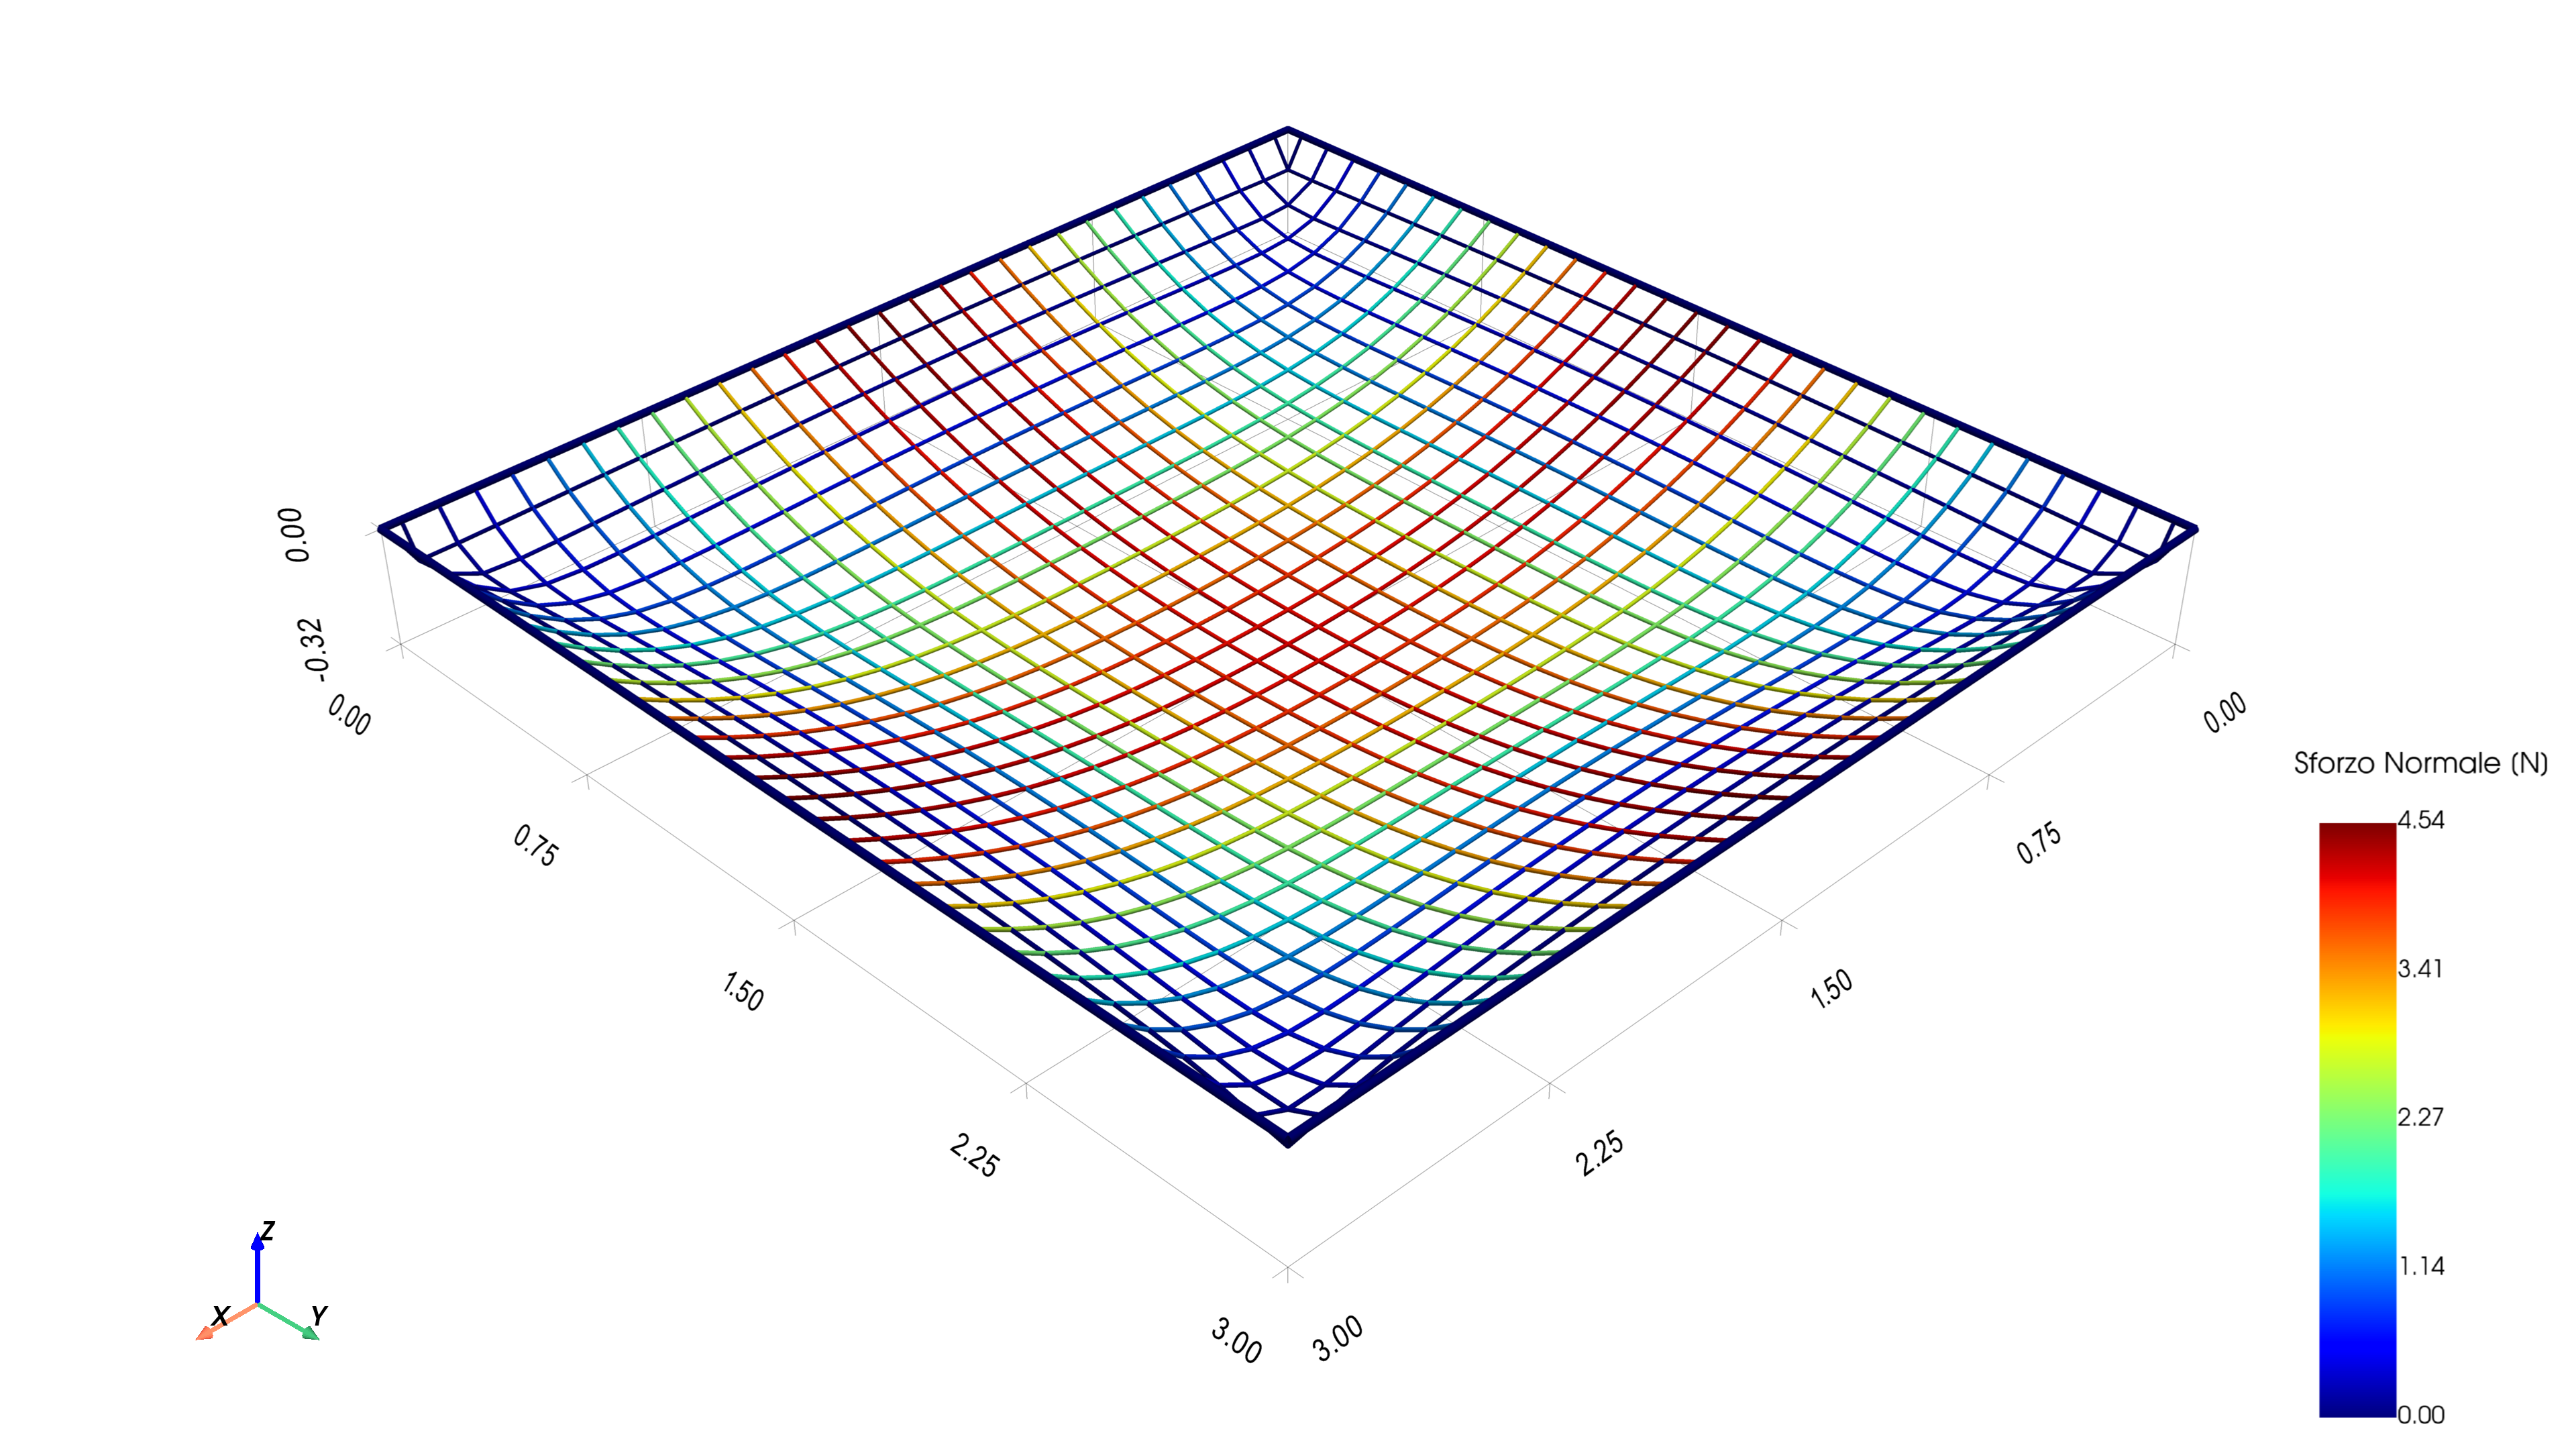
\includegraphics[width=\textwidth]{143_capitoli/capitolo2/immagini_capitolo_2/immagini_vincoli/rete_vincolata_4lati.png}
    \caption{Rete vincolata su 4 lati con cerniere mobili}
    \label{fig:rete_vincolata_4lati}
\end{figure}

\begin{figure}[H]
    \centering
    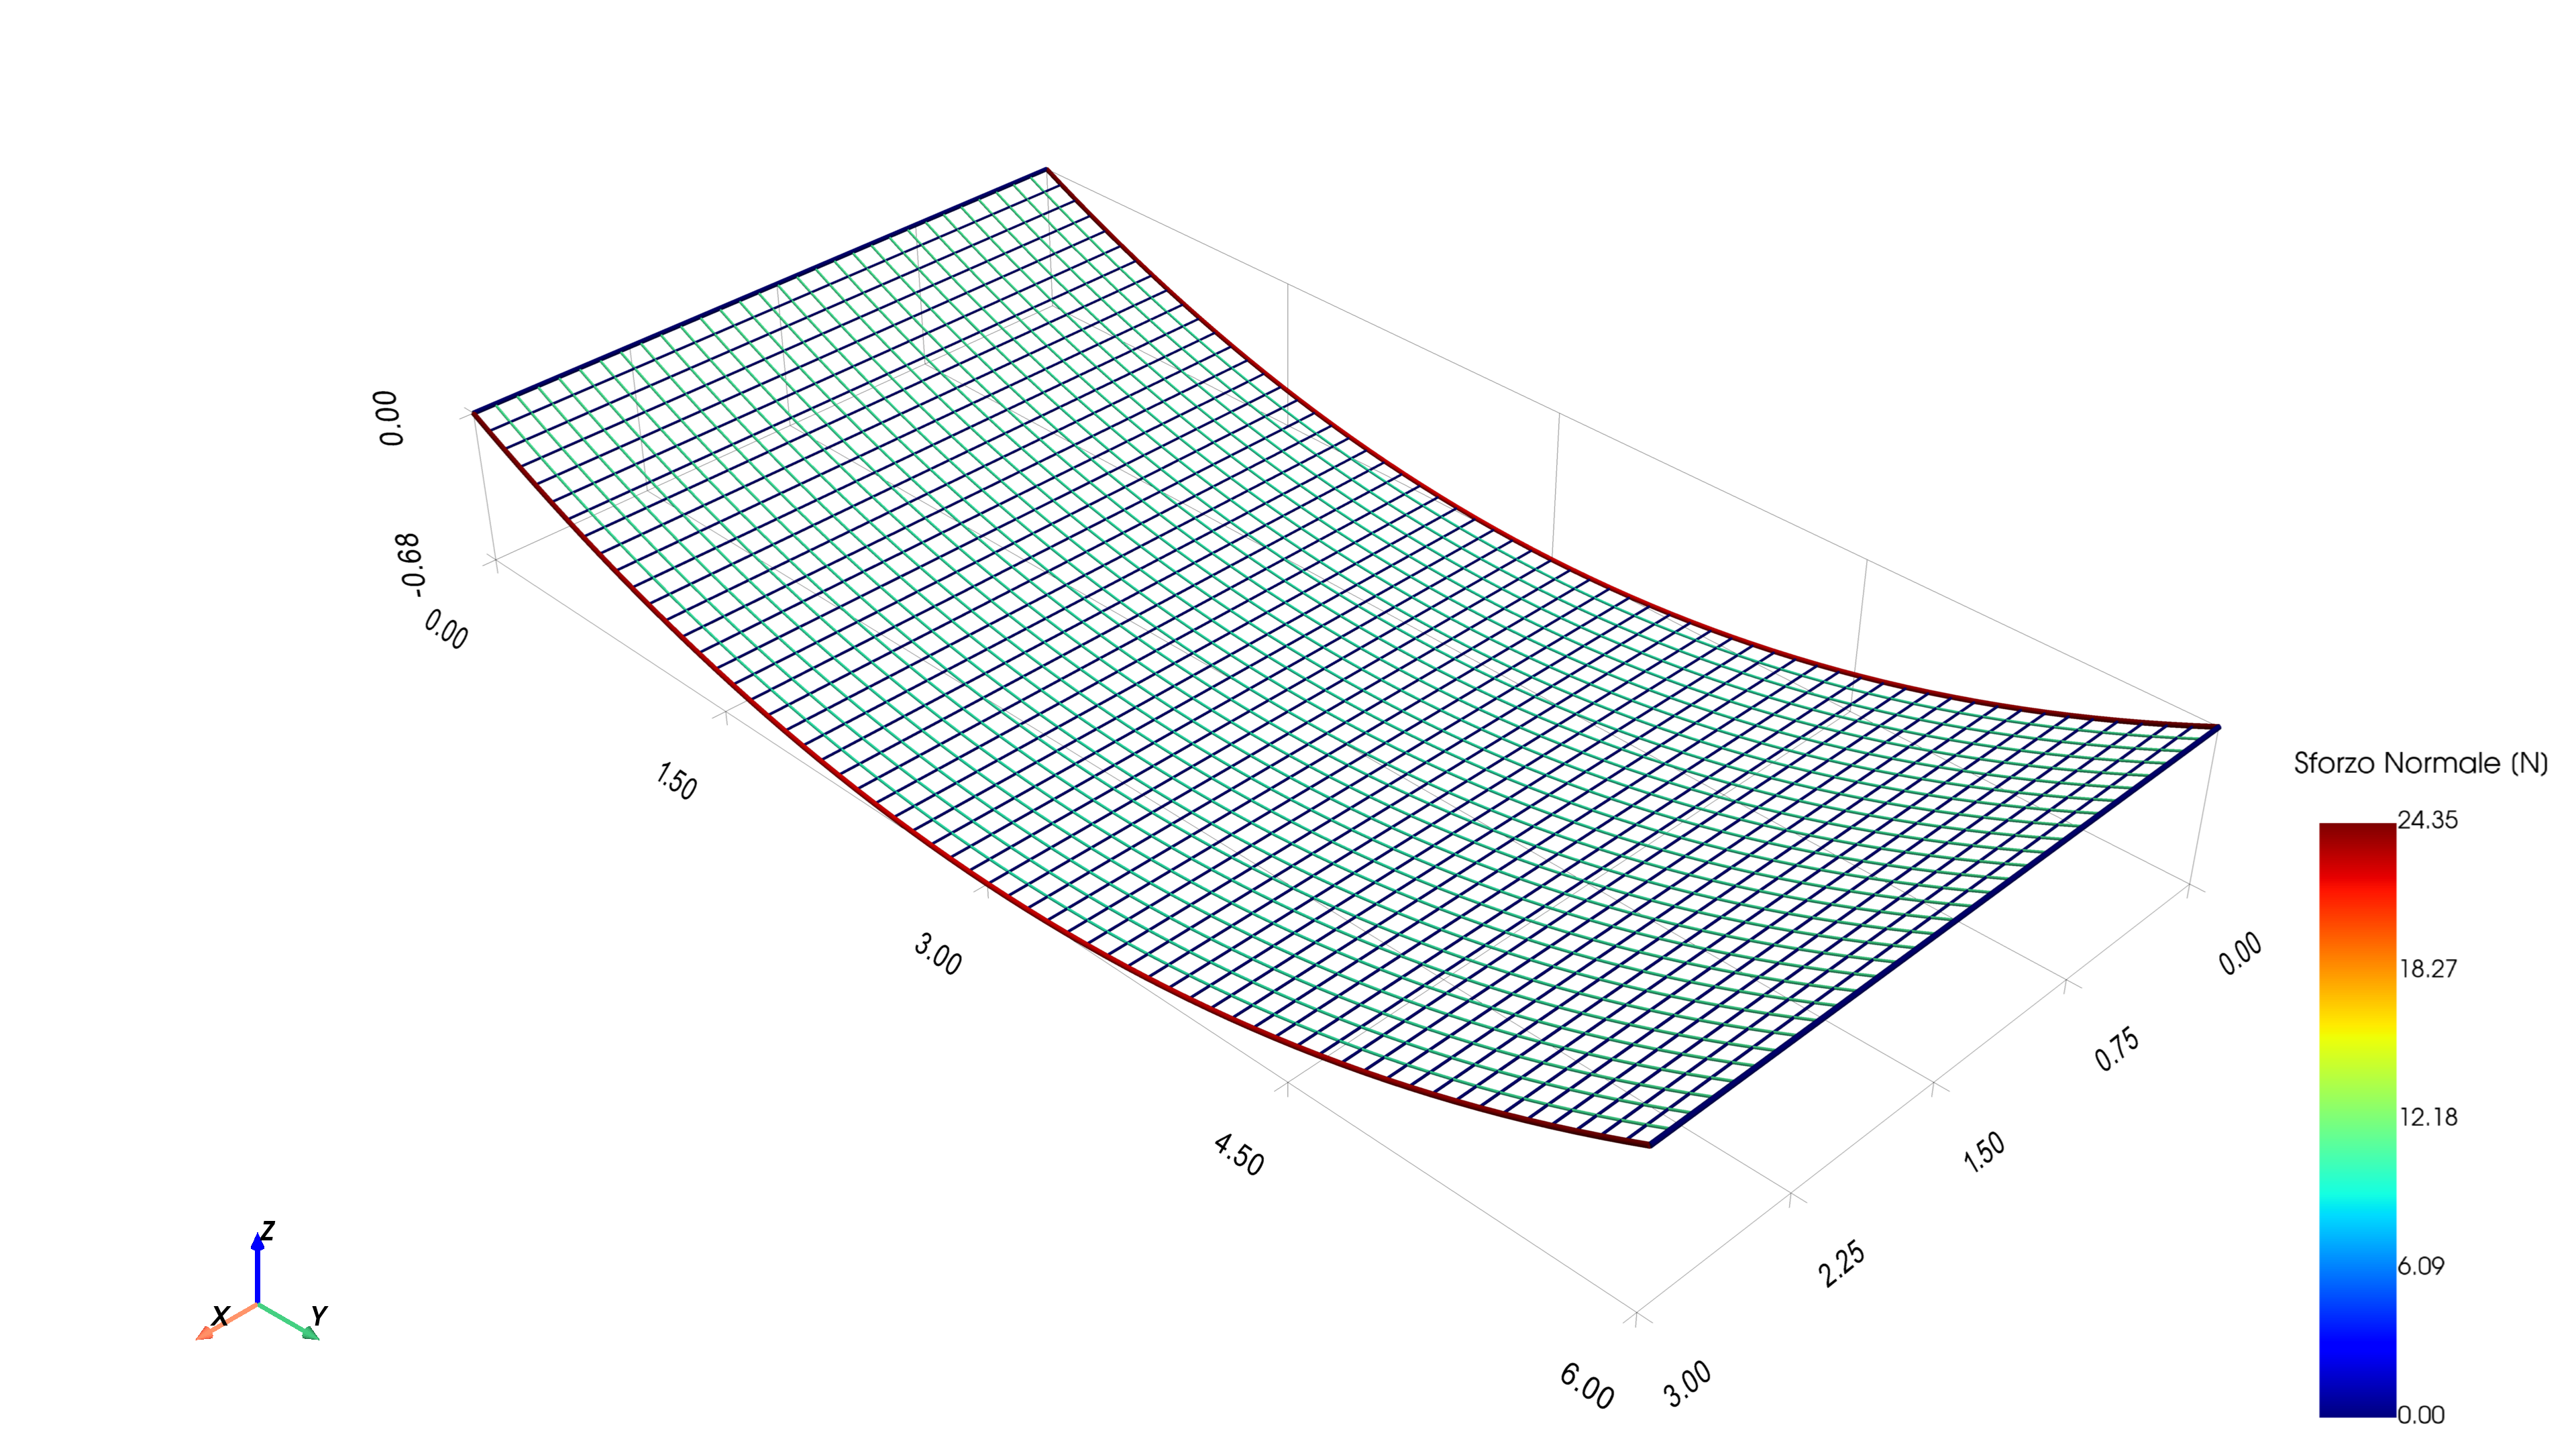
\includegraphics[width=\textwidth]{143_capitoli/capitolo2/immagini_capitolo_2/immagini_vincoli/rete_vincolata_x.png}
    \caption{Rete vincolata lungo i lati paralleli alla direzione 'x'}
    \label{fig:rete_vincolata_x}
\end{figure}

\begin{figure}[H]
    \centering
    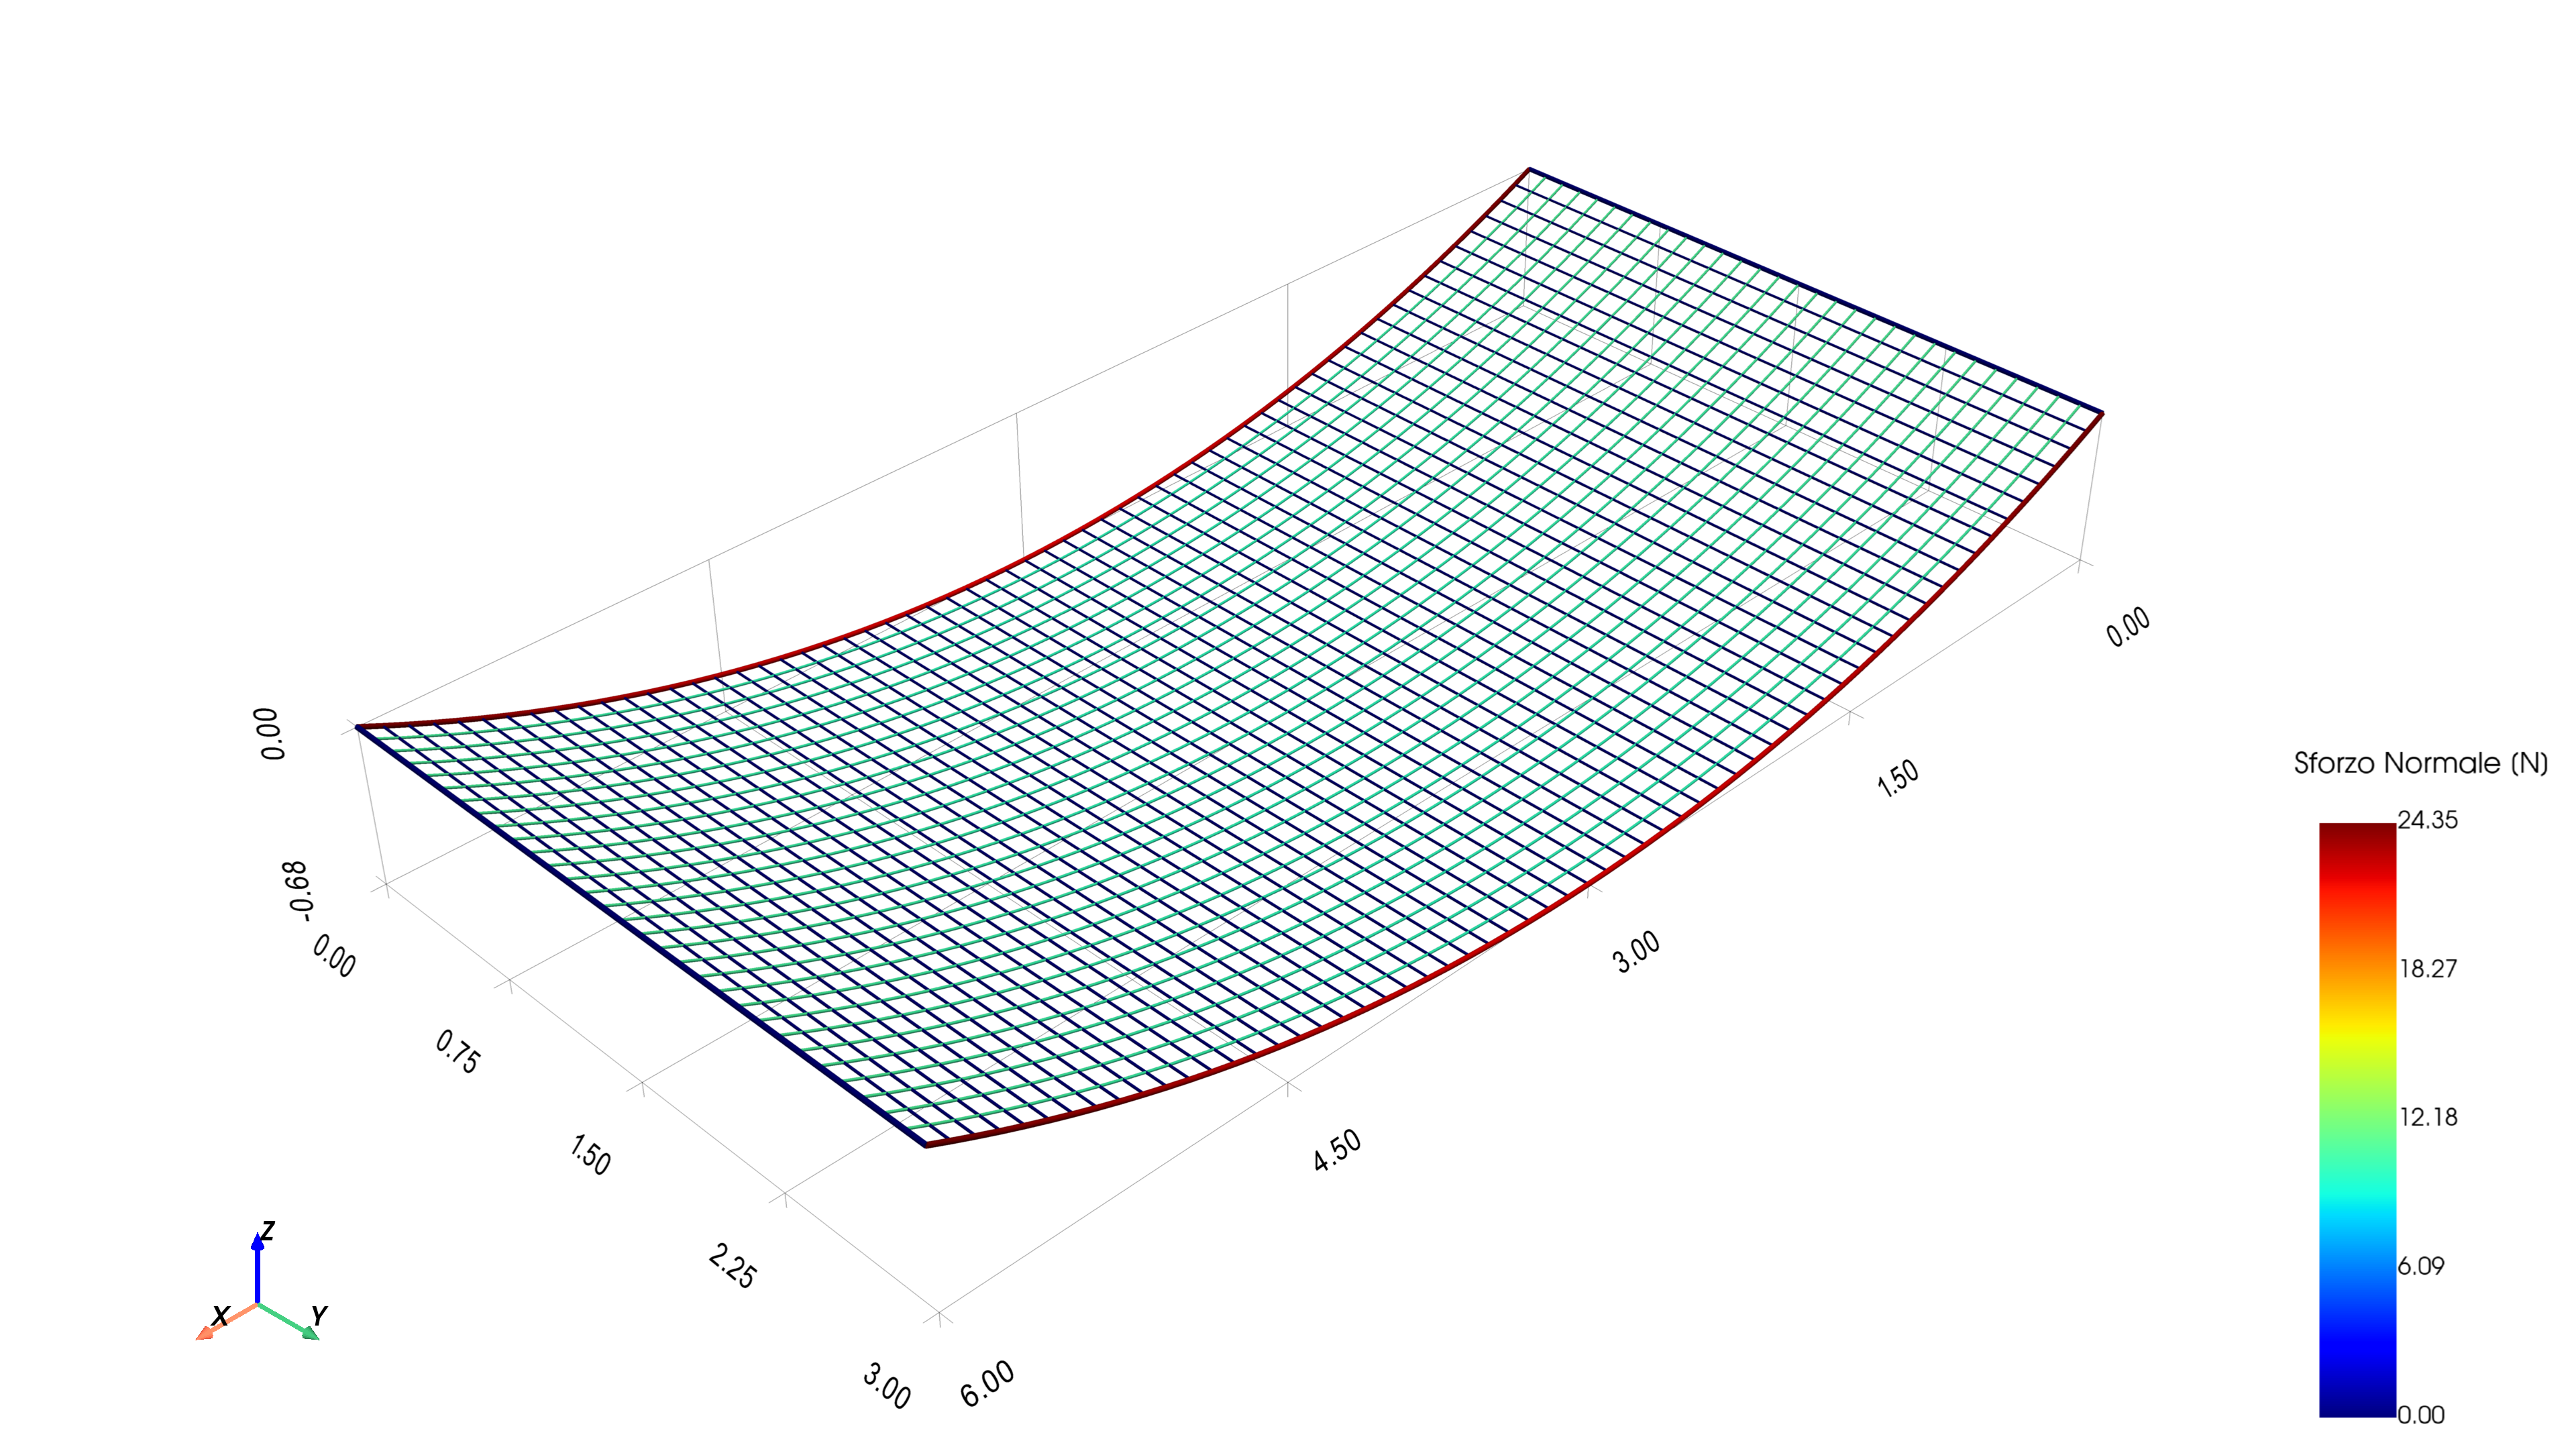
\includegraphics[width=\textwidth]{143_capitoli/capitolo2/immagini_capitolo_2/immagini_vincoli/rete_vincolata_y.png}
    \caption{Rete vincolata lungo i lati paralleli alla direzione 'y'}
    \label{fig:rete_vincolata_y}
\end{figure}

\begin{figure}[H]
    \centering
    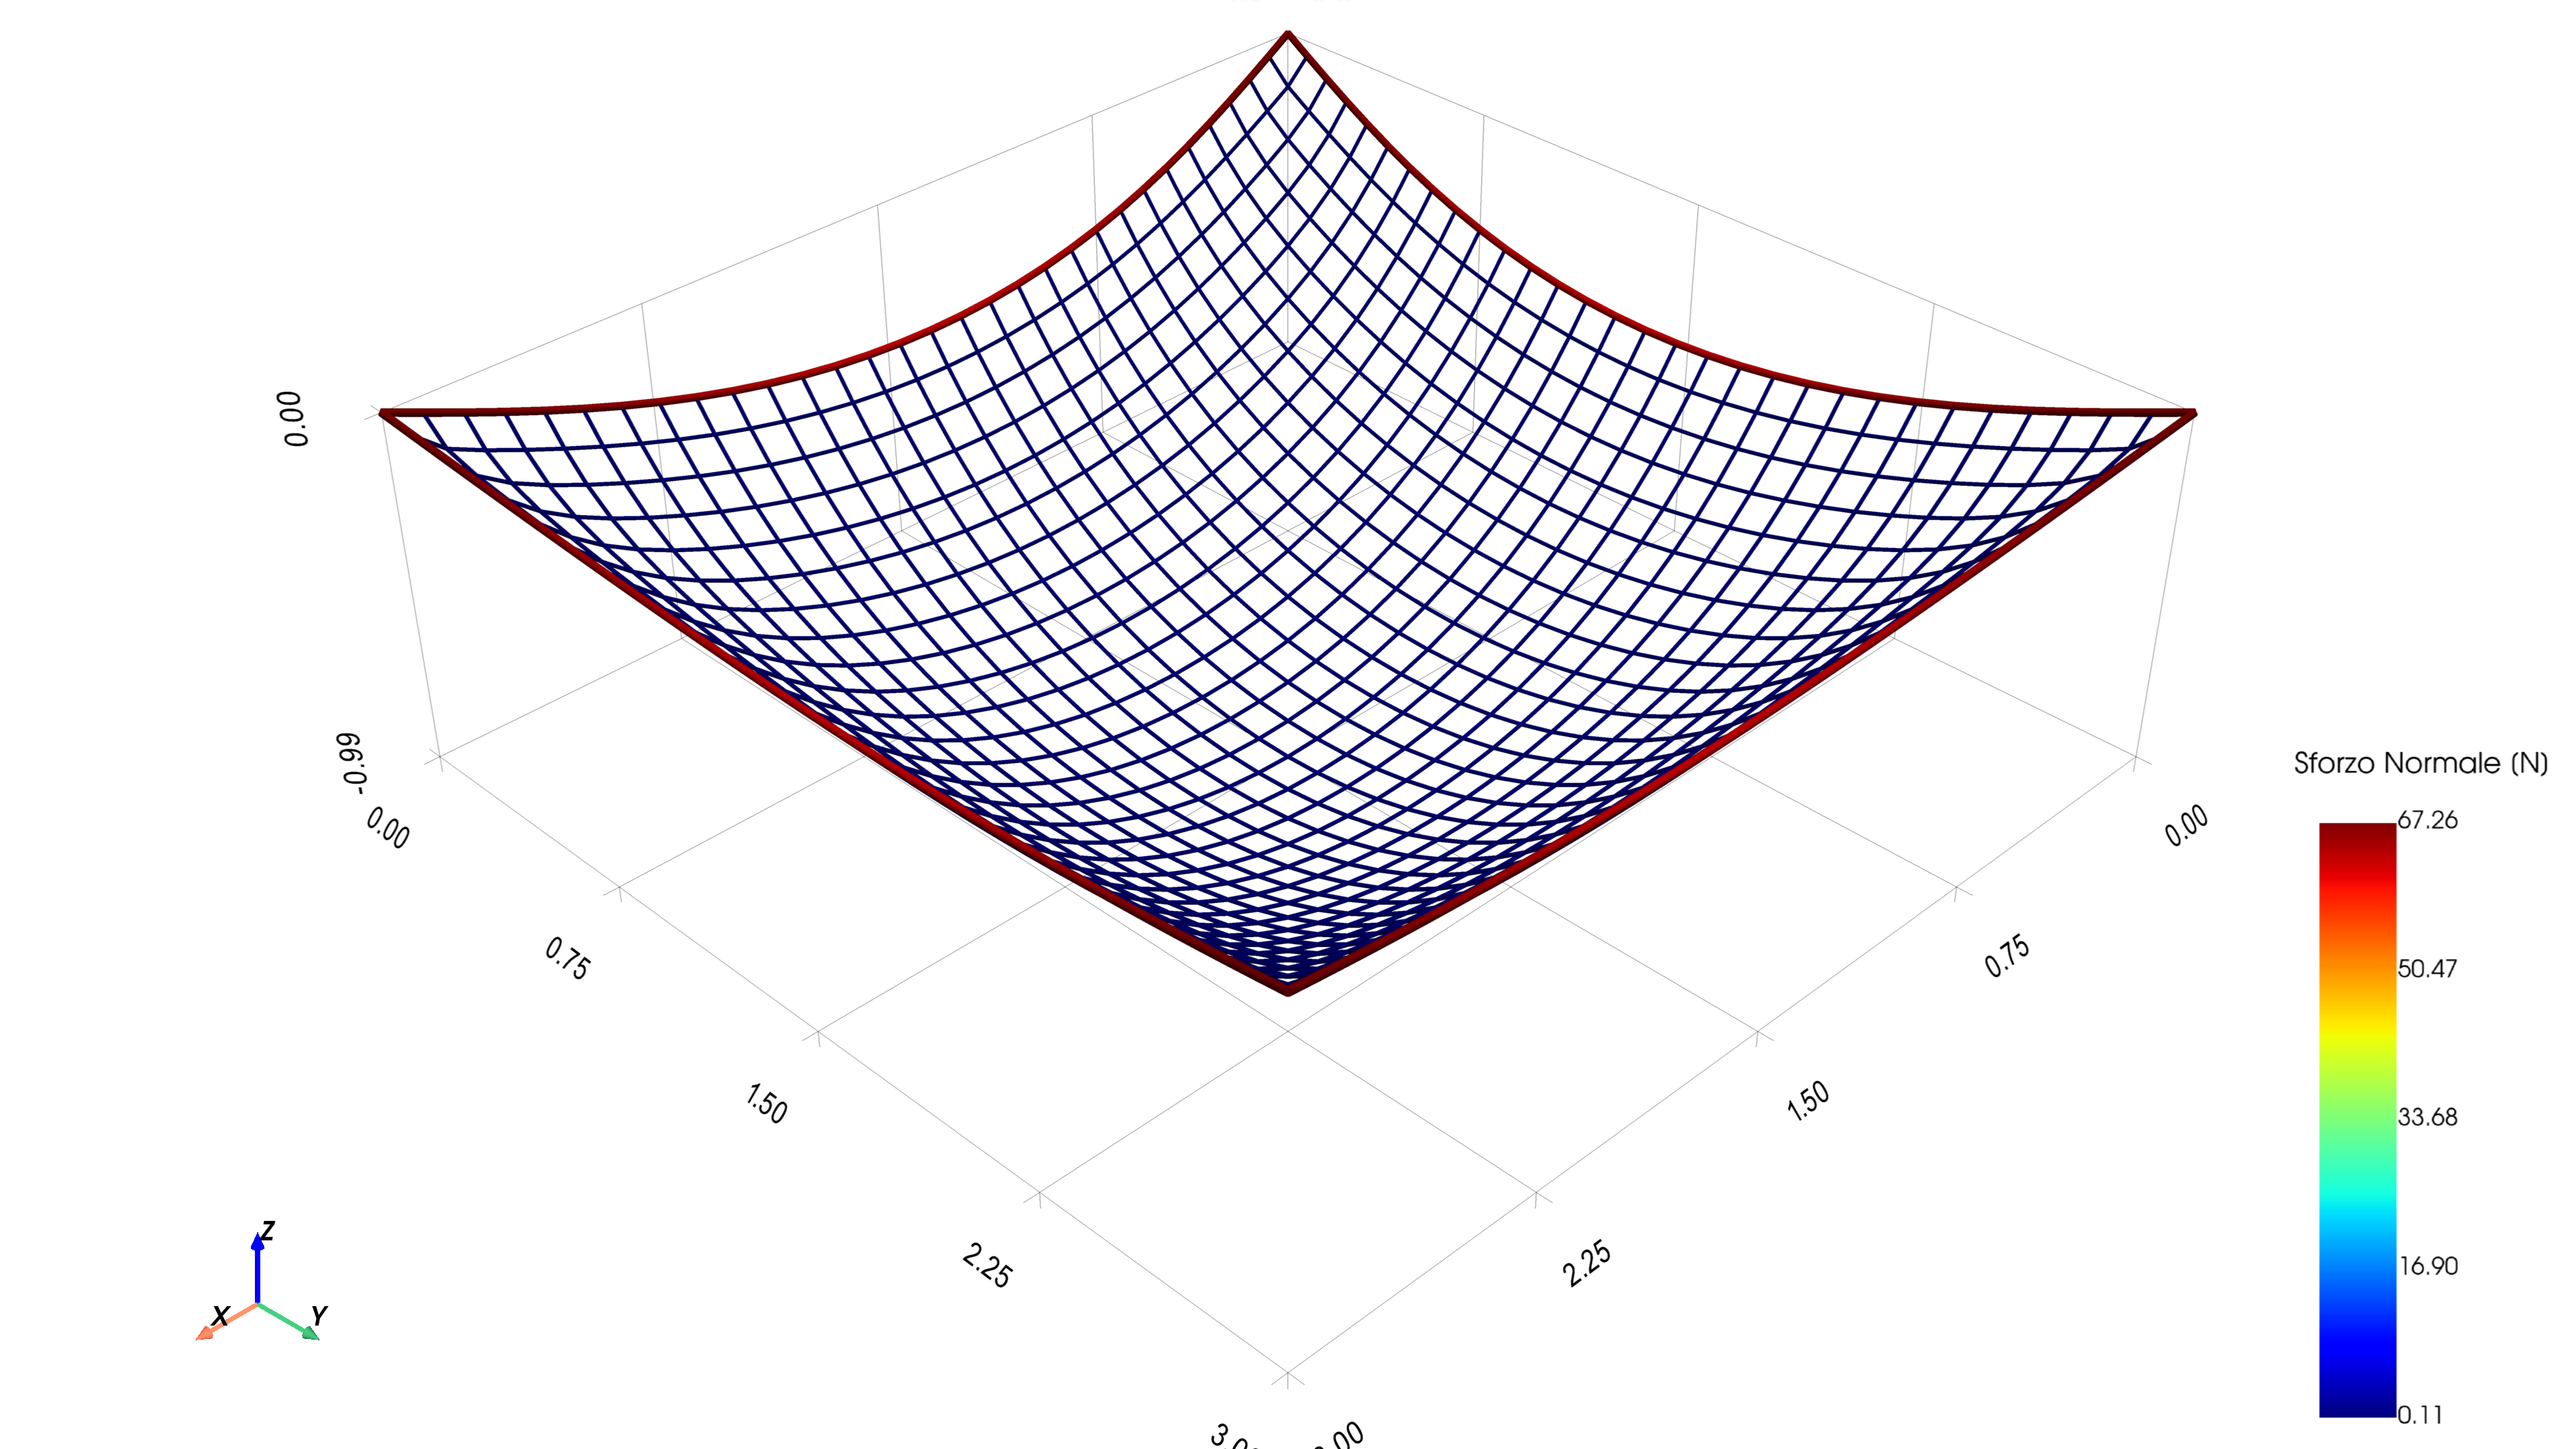
\includegraphics[width=\textwidth]{143_capitoli/capitolo2/immagini_capitolo_2/immagini_vincoli/rete_vincolata_corners.png}
    \caption{Rete vincolata ai nodi d'angolo}
    \label{fig:rete_vincolata_corners}
\end{figure}

\subsection{Area dei cavi}
Come noto dalla Scienza delle Costruzioni, la distribuzione delle forze all'interno di un sistema iperstatico è influenzata dalla ripartizione della rigidezza elastica tra gli elementi strutturali partecipanti. 

Nel caso specifico di strutture a comportamento fortemente non lineare per geometria, in cui l'ipotesi di piccoli spostamenti decade, la risoluzione numerica richiede l'impiego della matrice di rigidezza tangente, definita secondo l'\cref{eq:rigidezza_meccanica_geometrica}. Tale operatore risulta funzione diretta della rigidezza assiale degli elementi e della loro distribuzione spaziale. Di conseguenza, la corretta applicazione delle proprietà sezionali delle funi governa sia l'evoluzione delle stato tensionale sia la convergenza del processo iterativo volto alla soluzione del problema non lineare. 

All'interno del solutore, la rigidezza assiale degli elementi è modellata assumendo il modulo di elasticità $E$ costante in funzione del materiale impiegato e variando l'area trasversale efficace $A$ mediante la definizione di un raggio fittizio dei cavi. E'necessario evidenziare come il raggio imposta alla sezione circolare degli elementi sia un parametro puramente fittizio: le funi reali, infatti, non sono costituite da solidi omogenei a sezione piena, bensì da trefoli orditi secondo specifiche configurazioni geometriche. La presenza di vuoti interstiziali e lo scorrimento relativo tra i fili fanno sì che l'area resistente effettiva $A$ e il modulo elastico equivalente $E$ differiscano significativamente dai corrispondenti valori geometrici di un cilindro compatto di pari diametro. 

Tuttavia, l'assunzione di un comportamento elastico lineare per il materiale (ipotesi pienamente verificata per i problemi di validazione analizzati nel presente paragrafo, in cui le reti sono soggette al solo peso proprio o a carichi concentrati di intensità contenuta) consente di ottenere risultati fisicamente realistici e proporzionali alla rigidezza relativa dei componenti. Sotto l'ipotesi che la variabilità della rigidezza reale sia correlata linearmente alla sezione efficace, il solutore descrive con sufficiente accuratezza il flusso delle forze interne in funzione dei rapporti di rigidezza imposti. 

Il solutore consente di modellare diverse distribuzioni di area trasversale:
\begin{itemize}
   \item Configurazione omogenea: tutti gli elementi fune del dominio presentano la stessa area trasversale;
   \item Configurazione differenziata a due vie: distinzione di proèprietà tra le funi costituenti la maglia interna e le funi di bordo (\textit{border rope});
   \item Configurazione differenziata a tre vie: si ha una caratterizzazione indipendendente per le funi di maglia, le funi di bordo e le funi poste sulle diagonali principali, ove presenti. 
\end{itemize}
Sulla base dello scenario voluto, l'algoritmo genera un vettore che associa a ciascun elemento strutturale, sfruttando l'ordinamento degli elementi visto in \cref{chap:connettività}, l'area corretta. Sviluppi futuri del codice potranno includere mappature ancor più flessibili a supporto della pregettazione. 

Di seguito si riportano i risultati ottenuti per una rete a maglia quadrata con funi di controvento, le cui caratteristiche geometriche e meccaniche sono riassunte in \cref{tab:caratteristiche_area_rete}.
\begin{table}[htbp]
    \centering
    \caption{Proprietà geometriche e meccaniche della rete a maglia quadrata con funi di controvento - analisi di sensibilità alla rigidezza.}
    \vspace{5pt}
    \label{tab:caratteristiche_area_rete}
    \begin{tabularx}{\textwidth}{l c X}
        \hline
        \textbf{Parametro} & \textbf{Simbolo} & \textbf{Valore nominale} \\ \hline
        Dimensione totale della rete & $L_x \times L_y$ & $3.00 \times 3.00$ $[\text{m}]$ \\
        Dimensione della singola maglia & $l_{m_x} \times l_{m_y}$ & $10 \times 10$ $[\text{cm}]$ \\
        Diametro nominale delle funi & $\phi _1$ & $5.0$ $[\text{mm}]$ \\
        Diametro nominale delle funi & $\phi _2$ & $10.0$ $[\text{mm}]$ \\
        Modulo di elasticità longitudinale fune & $E$ & 2.1e9 $[\text{Pa}]$ \\
        Area della sezione trasversale fune & $A_1$ & 19.63 $[\text{mm}^2]$ \\
        Area della sezione trasversale fune & $A_2$ & 78.54 $[\text{mm}^2]$ \\
        Bando iniziale cinematico - x (Slackness) & $L_x/l_x$ & 0 $[\text{\%}]$ \\
        Bando iniziale cinematico - y (Slackness) & $L_y/l_y$ & 0 $[\text{\%}]$ \\ \hline
    \end{tabularx}
\end{table}

\begin{figure}[H]
    \centering
    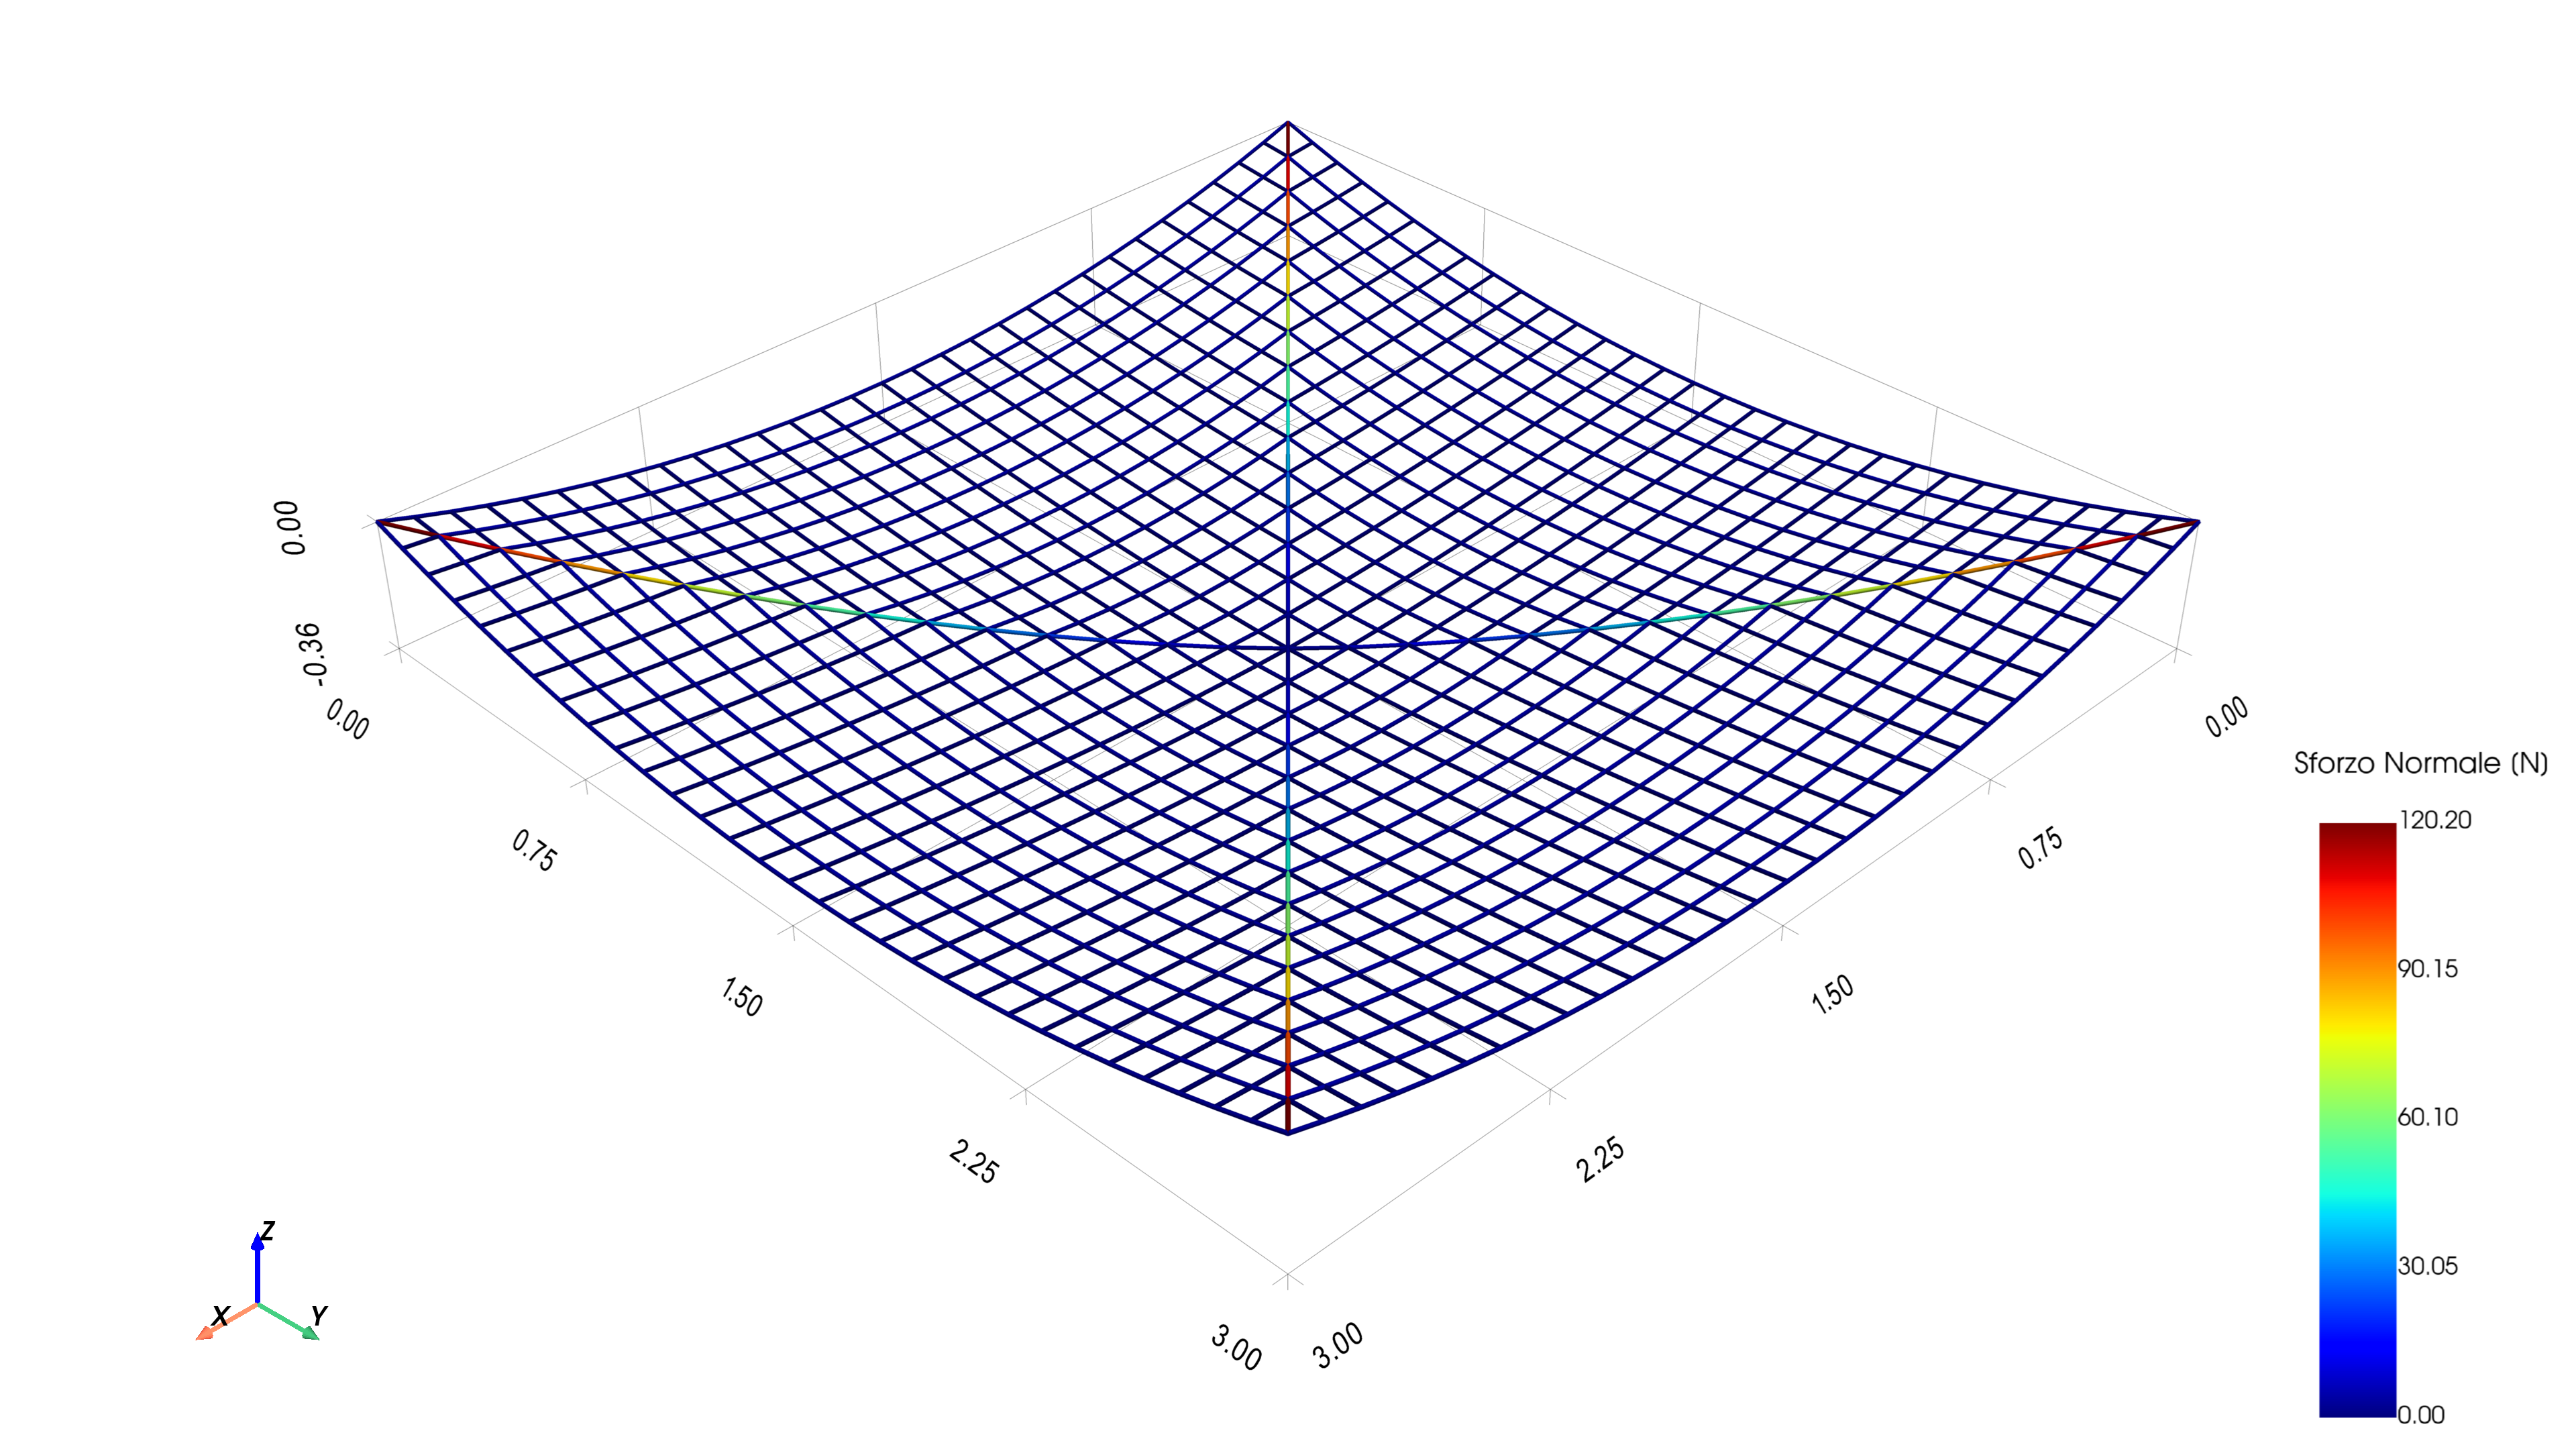
\includegraphics[width=\textwidth]{143_capitoli/capitolo2/immagini_capitolo_2/immagini_area/rete_aree_uguali.png}
    \caption{Rete con configurazione omogenea delle aree degli elementi fune}
    \label{fig:rete_aree_uguali}
\end{figure}

\begin{figure}[H]
    \centering
    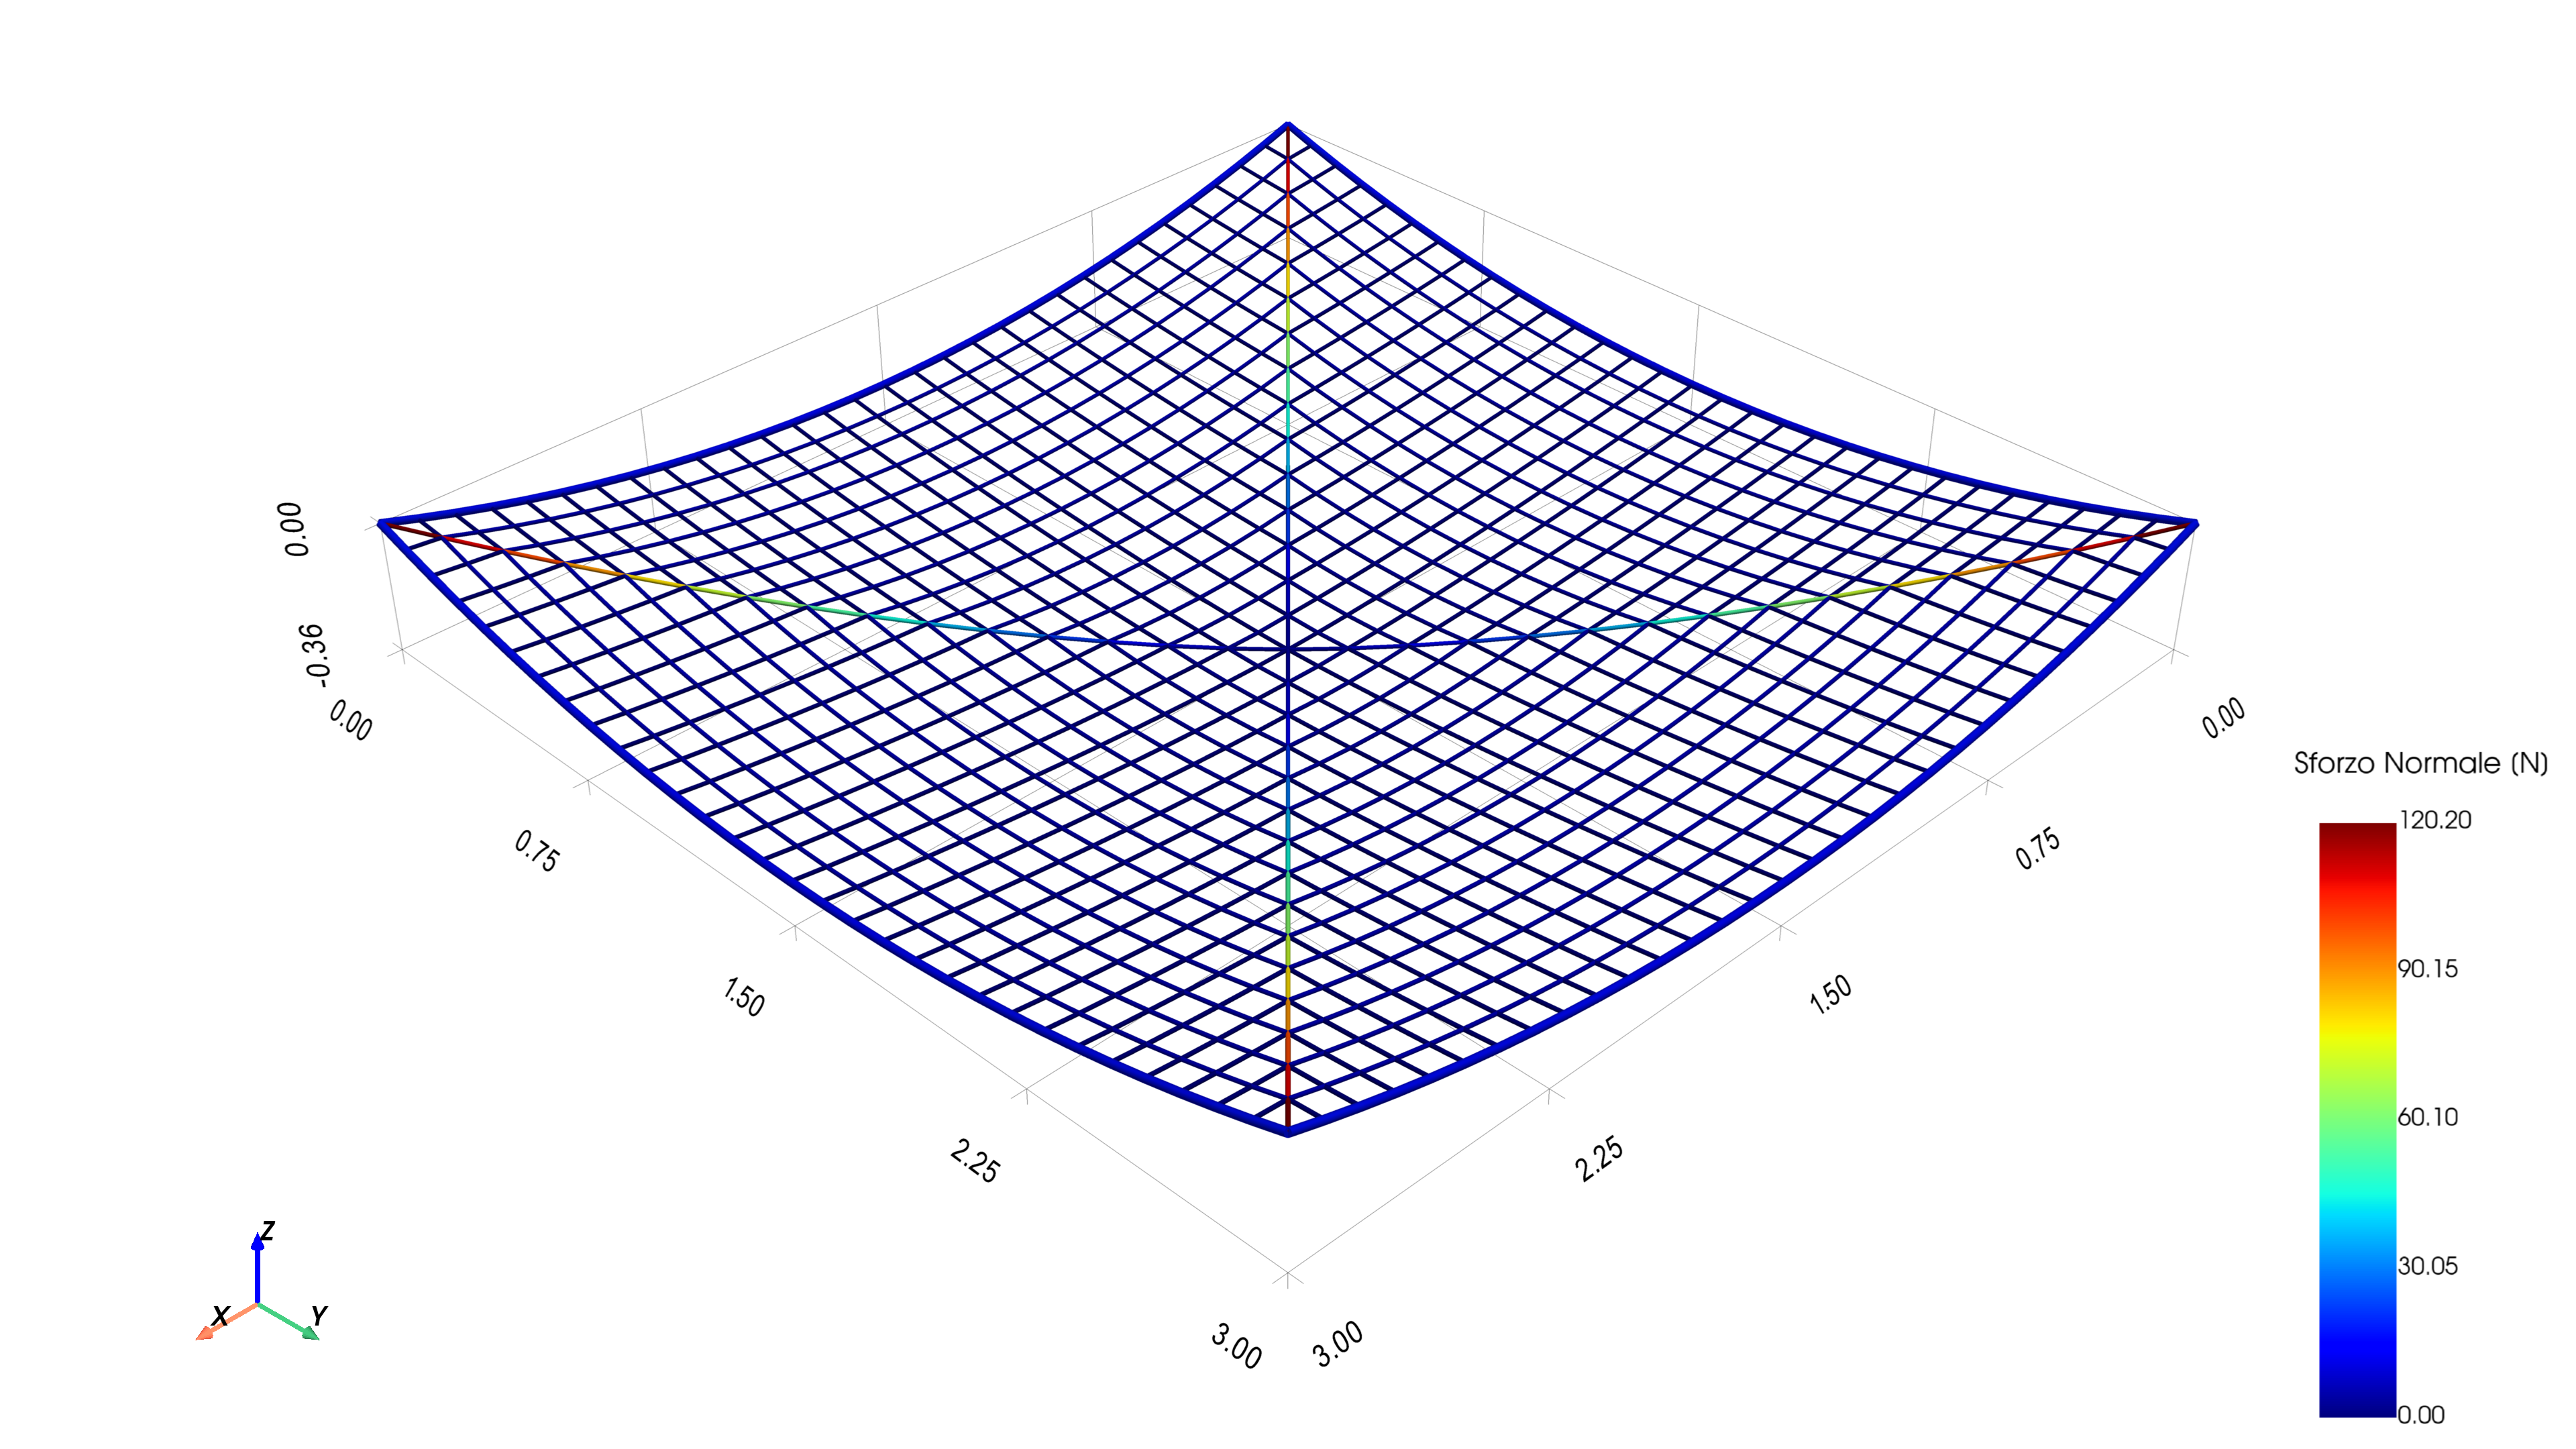
\includegraphics[width=\textwidth]{143_capitoli/capitolo2/immagini_capitolo_2/immagini_area/rete_aree_differenti1.png}
    \caption{Rete con configurazione differenziata a due vie delle aree degli elementi fune}
    \label{fig:rete_aree_diffenti1}
\end{figure}

\begin{figure}[H]
    \centering
    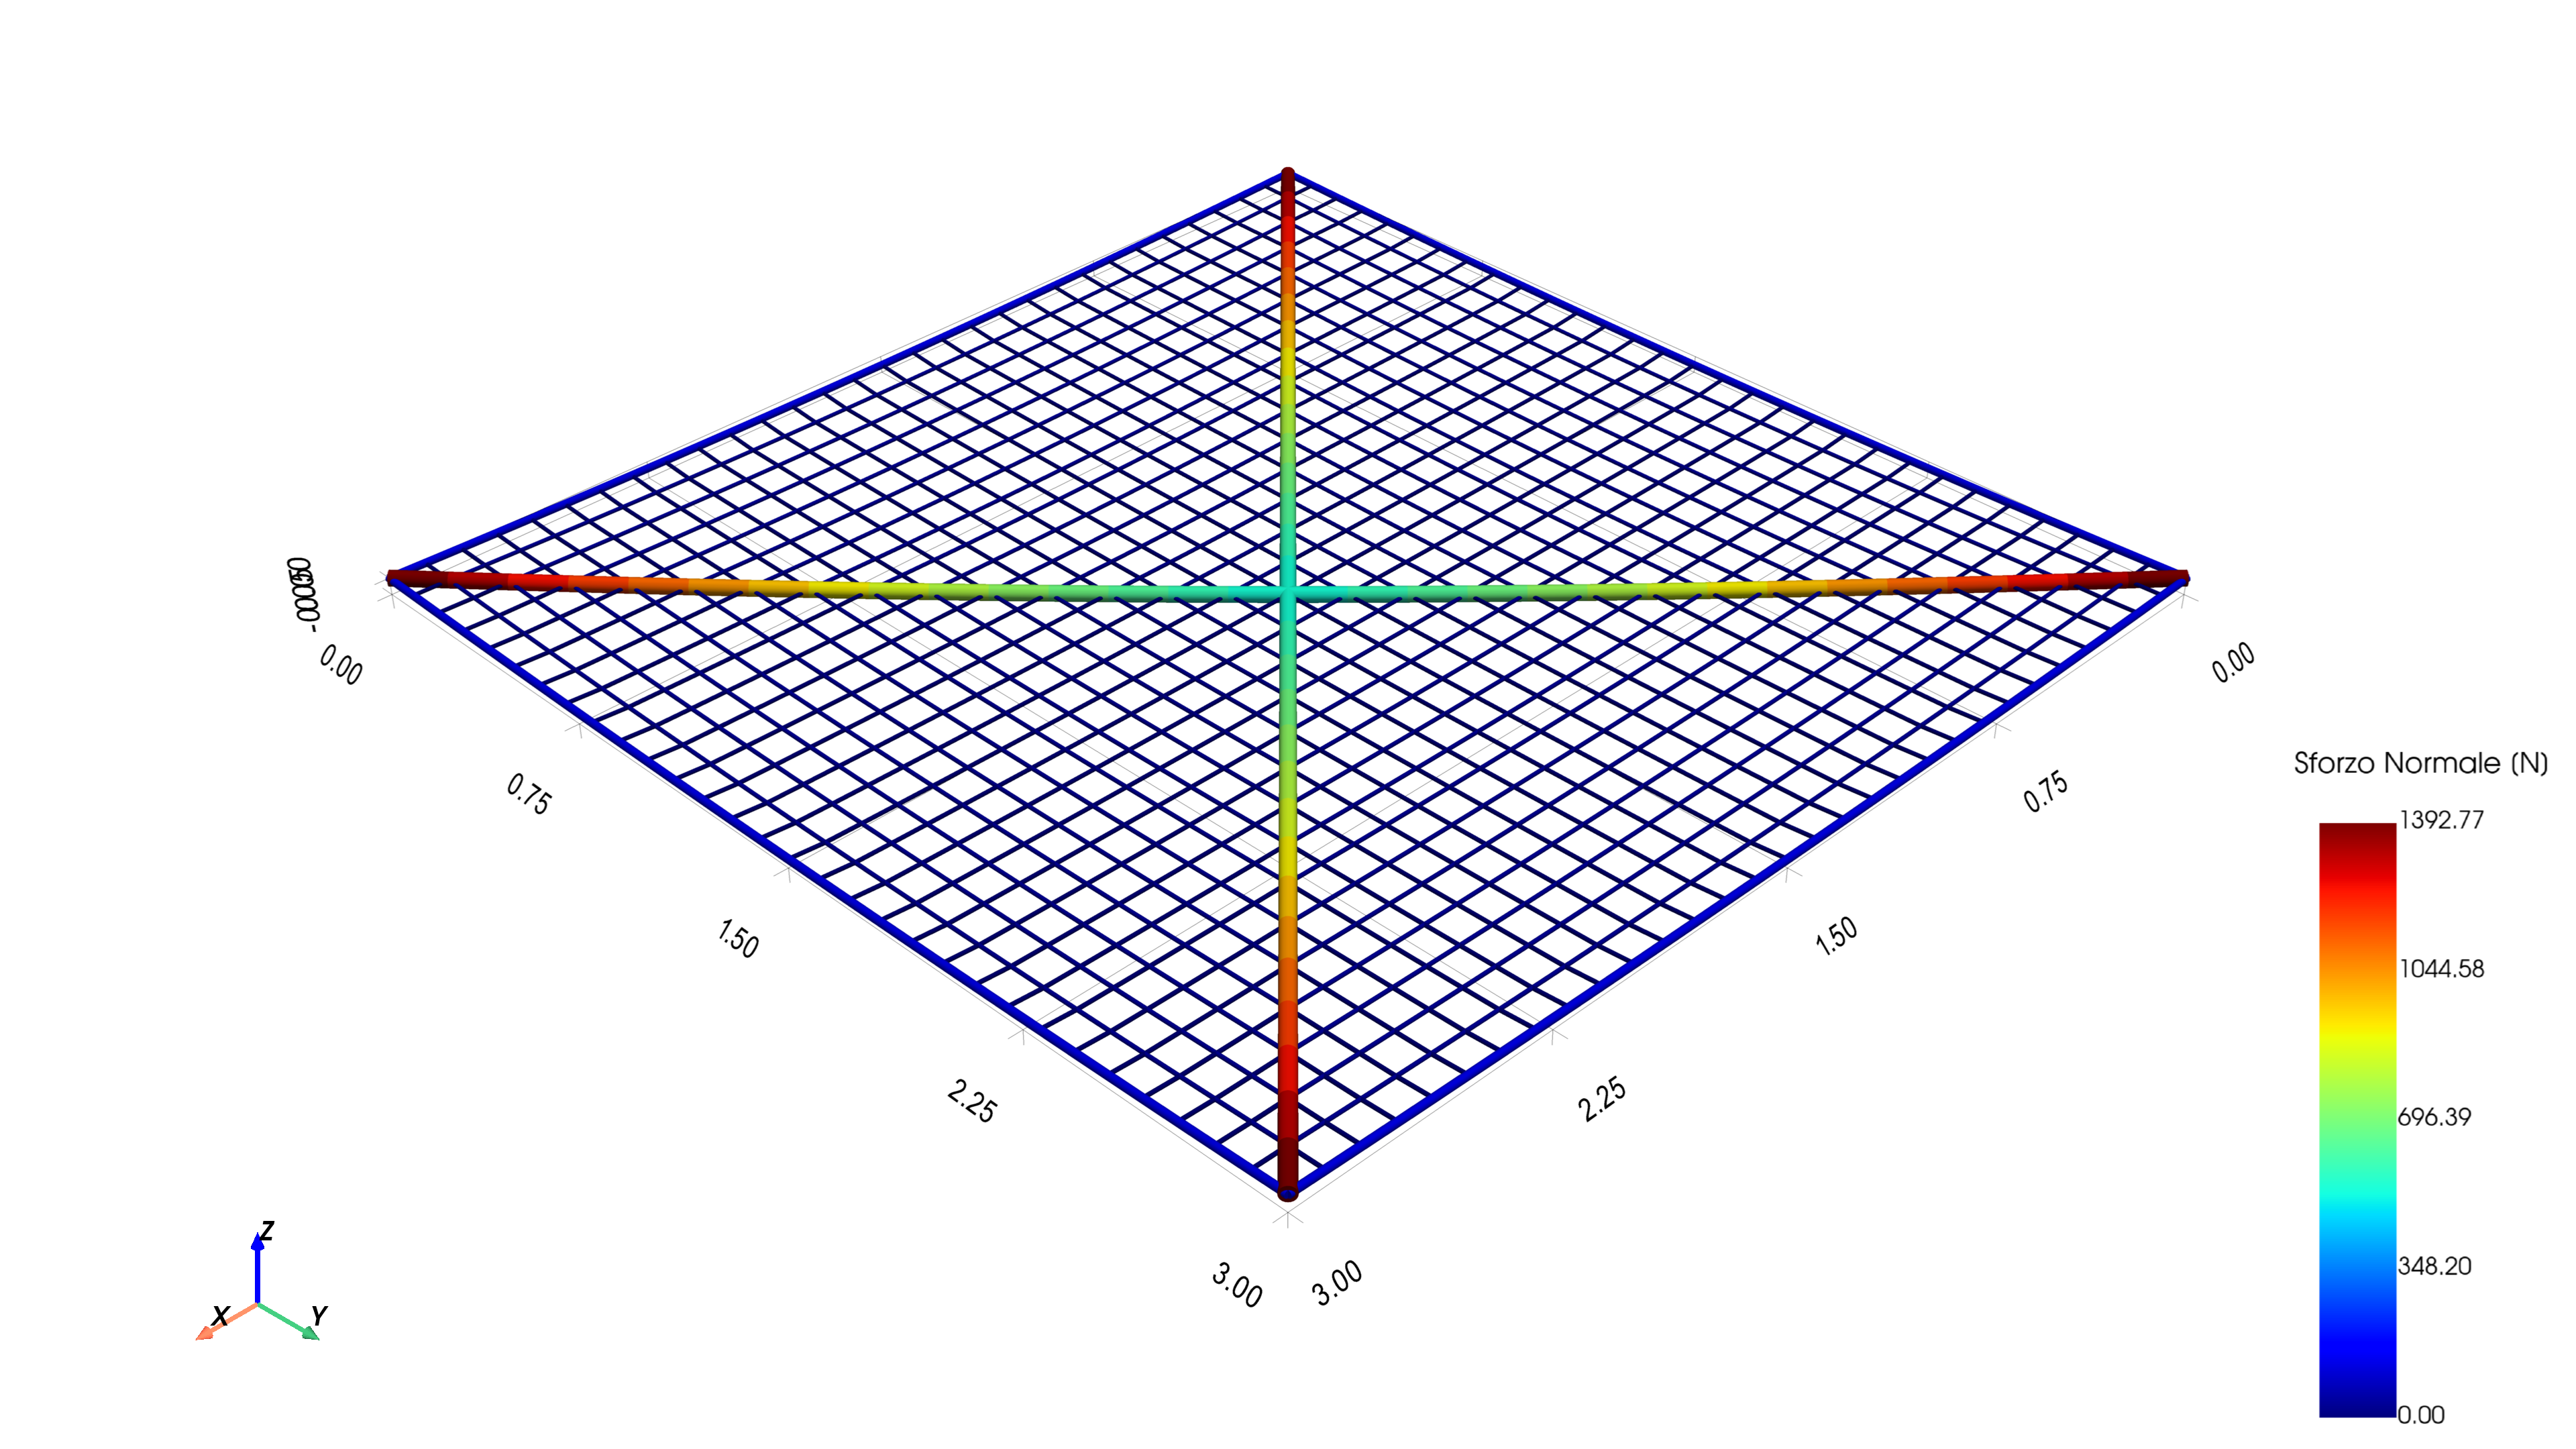
\includegraphics[width=\textwidth]{143_capitoli/capitolo2/immagini_capitolo_2/immagini_area/rete_aree_differenti2.png}
    \caption{Rete con configurazione differenziata a tre vie delle aree degli elementi fune}
    \label{fig:rete_aree_differenti2}
\end{figure}

\subsection{Il fenomeno dello \textit{slack} nelle reti di cavi}
Nella trattazione della fune monodimensionale soggetta al peso proprio, qualora la lunghezza del suo sviluppo risulti superiore alla distanza lineare tra i vincoli di estremità, si definisce la condizione di fune \textit{lasca} o di \textit{slack}. In tale configurazione, la fune si trova in bando ed è caratterizzata da un tiro orizzontale poco significativo. 

In modo analogo, per sistemi discreti bidimensionali si utilizza la dicitura di rete lasca (\textit{net cables with slack}) per indicare una rete in cui lo sviluppo geometrico dei cavi costituenti è maggiore della distanza tra i vincoli perimetrali. Di conseguenza la rete non risulterà soggetta a tensioni elevate in direzione ortogonale a quella dei lati vincolati Tuttavia, il caso in cui entrambi i lati della maglia siano più lunghi dei rispettivi lati vincolati introduce una complessità analitica e strutturale superiore rispetto al caso monodimensionale. 

Il fenomeno dello \textit{slack} si verifica in maniera differenziata in funzione della geometria della mesh assunta: 
\begin{itemize}
    \item Rete a maglia quadrata (\textit{squared mesh} (Q)): se lungo le direzioni principali dell'orditura ($x$ e $y$) lo stato tensionale è idealmente dominato da sforzi normali di trazione, lungo le direzioni inclinate gli sforzi di trazione generano sollecitazioni di taglio. Lungo le diagonali principali che uniscono gli angoli, perciò, avremo una sollecitazione di trazione massima, a cui corrisponde in direzione ortogonale una compressione. Come visibile dai risultati riportati in figura \cref{fig:rete_Q_slack}, si creano delle zone del dominio della rete in cui molti elementi vanno in \textit{slack} perchè compressi.
    \item Rete a maglia romboidale (\textit{diamond mesh} (D)): in questo caso, la maglia risultata ruotata di $45^\circ$ rispetto alla precedente. Di conseguenza la direzione in cui si verifica lo \textit{slack} è ortogonale rispetto al caso della mesh quadrata, come visibile in \cref{fig:rete_D_slack}. Assumendo un dominio in cui  $L_y = L_x = L$, le diagonali di lunghezza $\sqrt{2} L$ rappresentano le direzioni in cui si localizzano i maggiori allungamenti del dominio, inducendo l'allentamento dei cavi disposti lungo le direzioni evidenziate.
\end{itemize}

\begin{figure}[H]
   \centering
    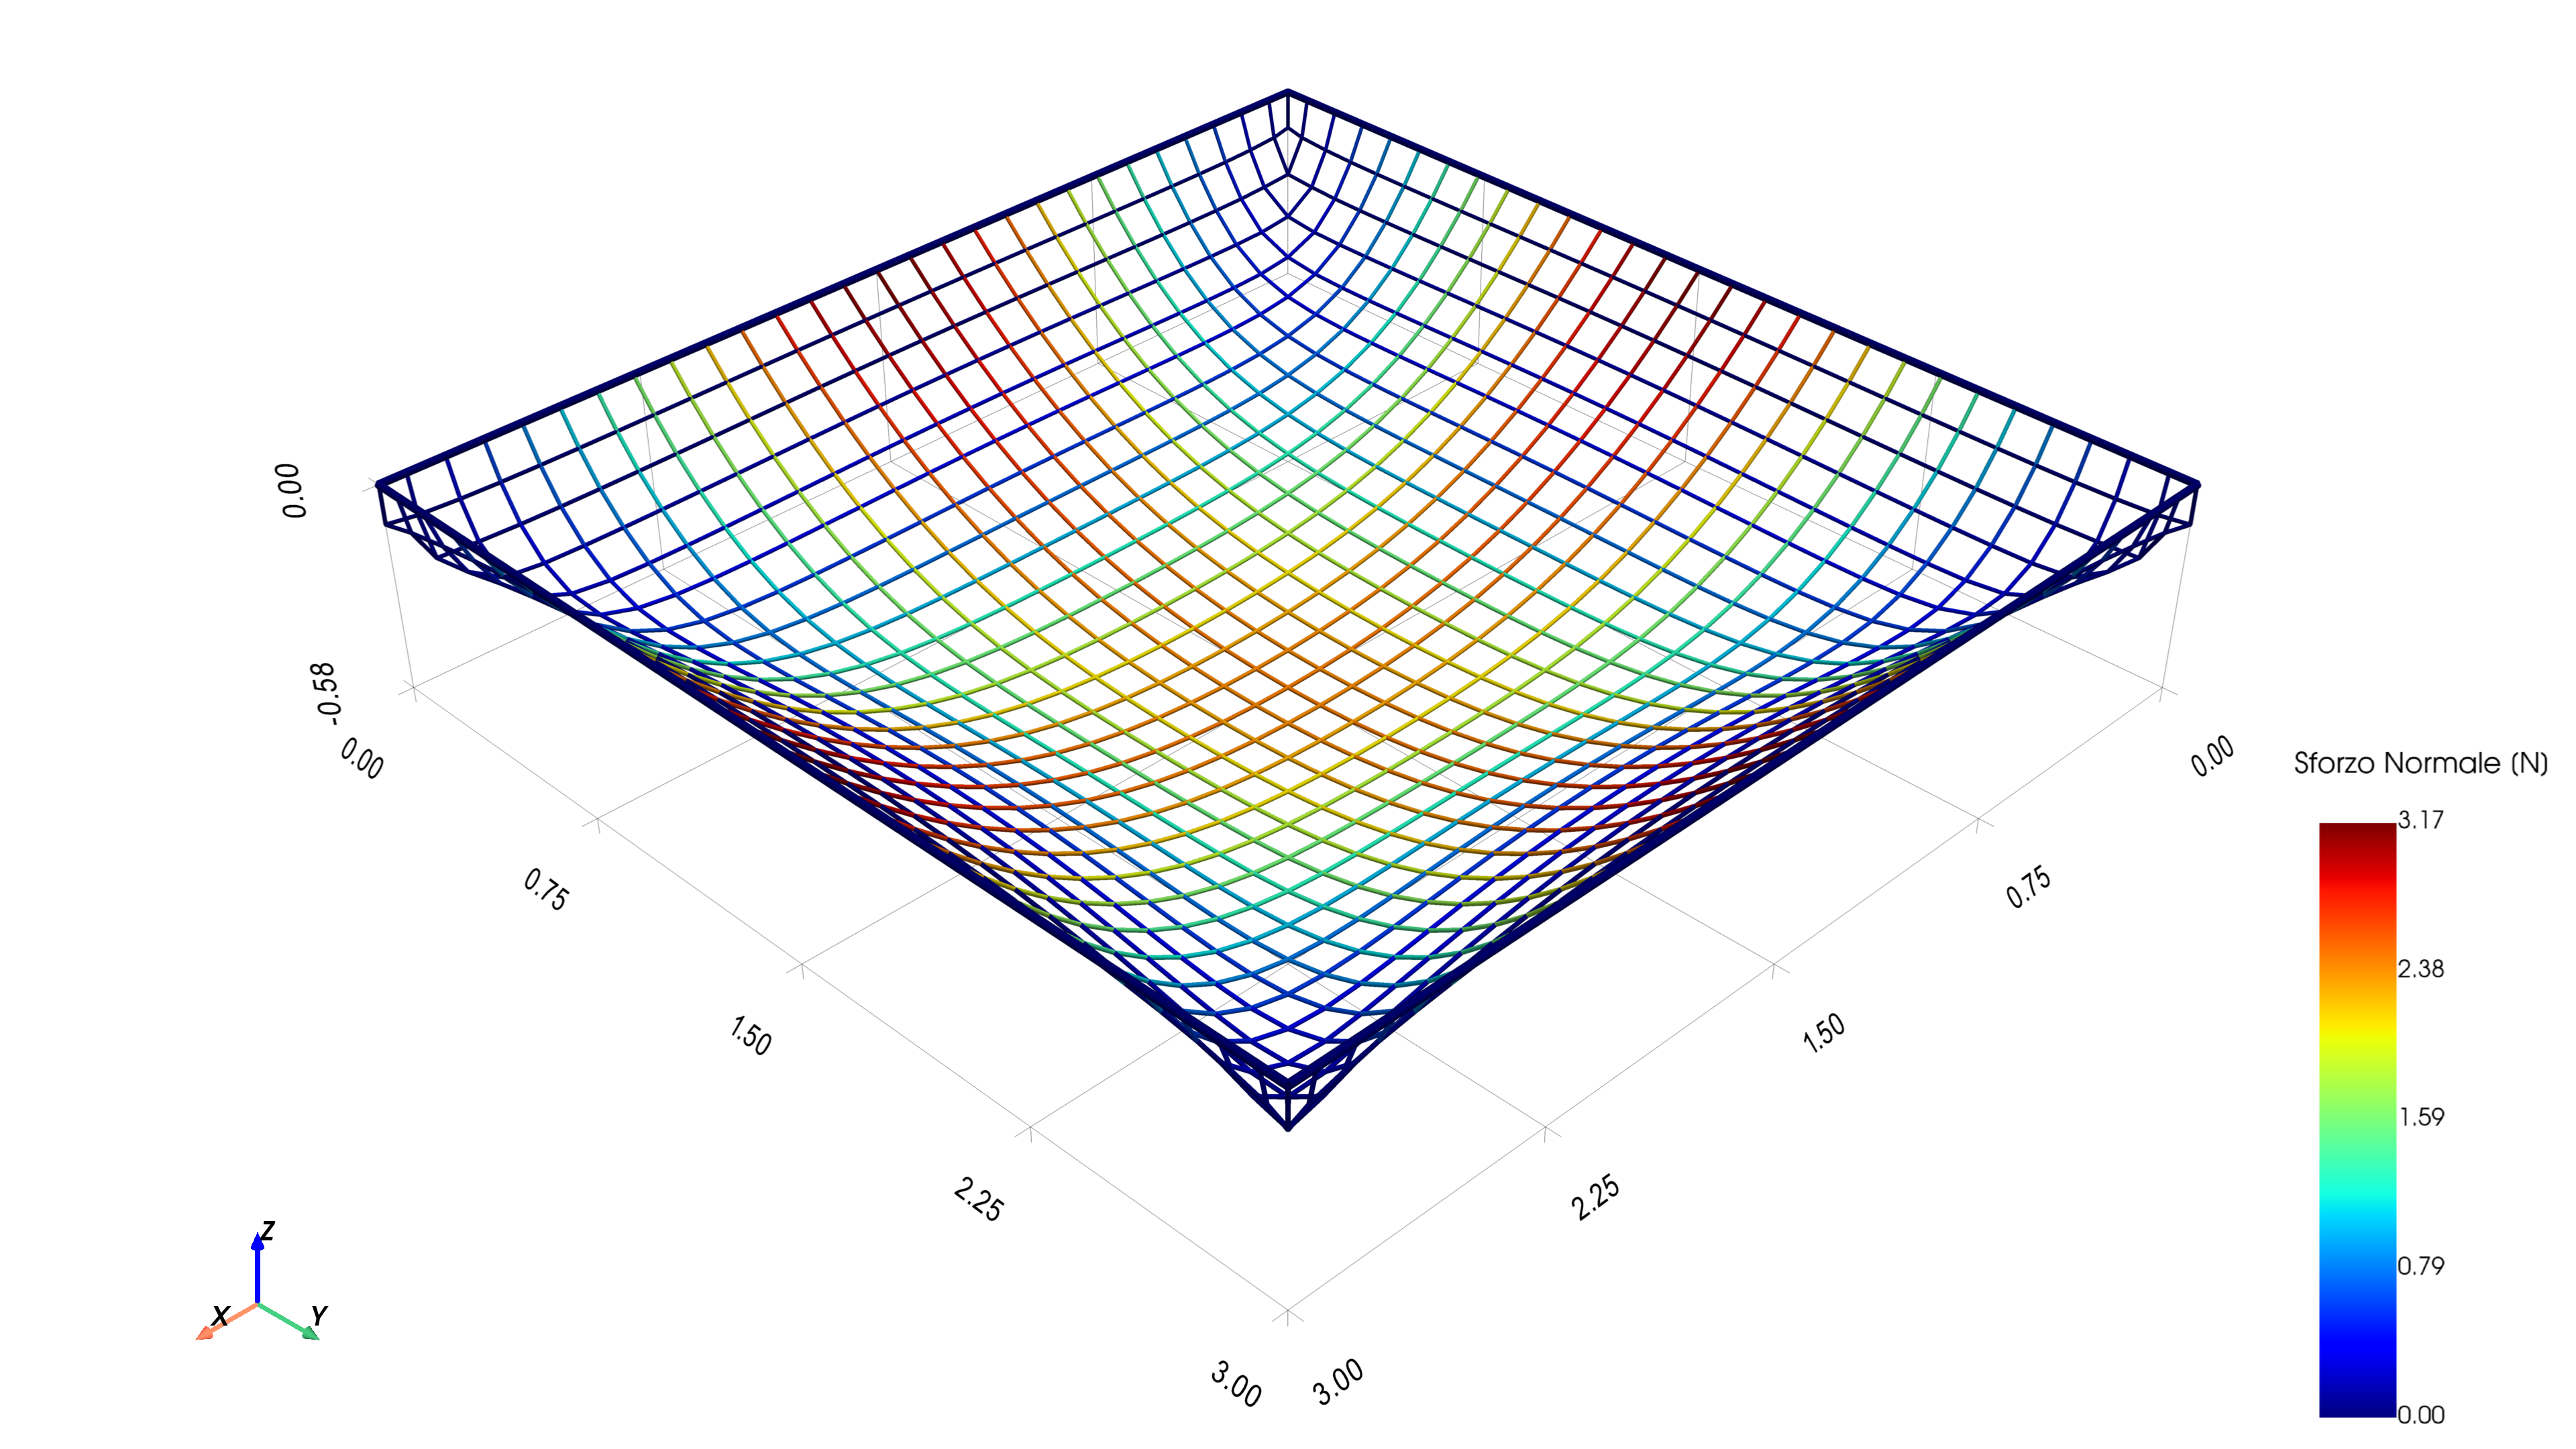
\includegraphics[width=\textwidth]{143_capitoli/capitolo2/immagini_capitolo_2/immagini_slack/rete_Q_slack.png}
    \caption{Rete a maglia quadrata in condizione di slack}
    \label{fig:rete_Q_slack}
\end{figure}

\begin{figure}[H]
   \centering
    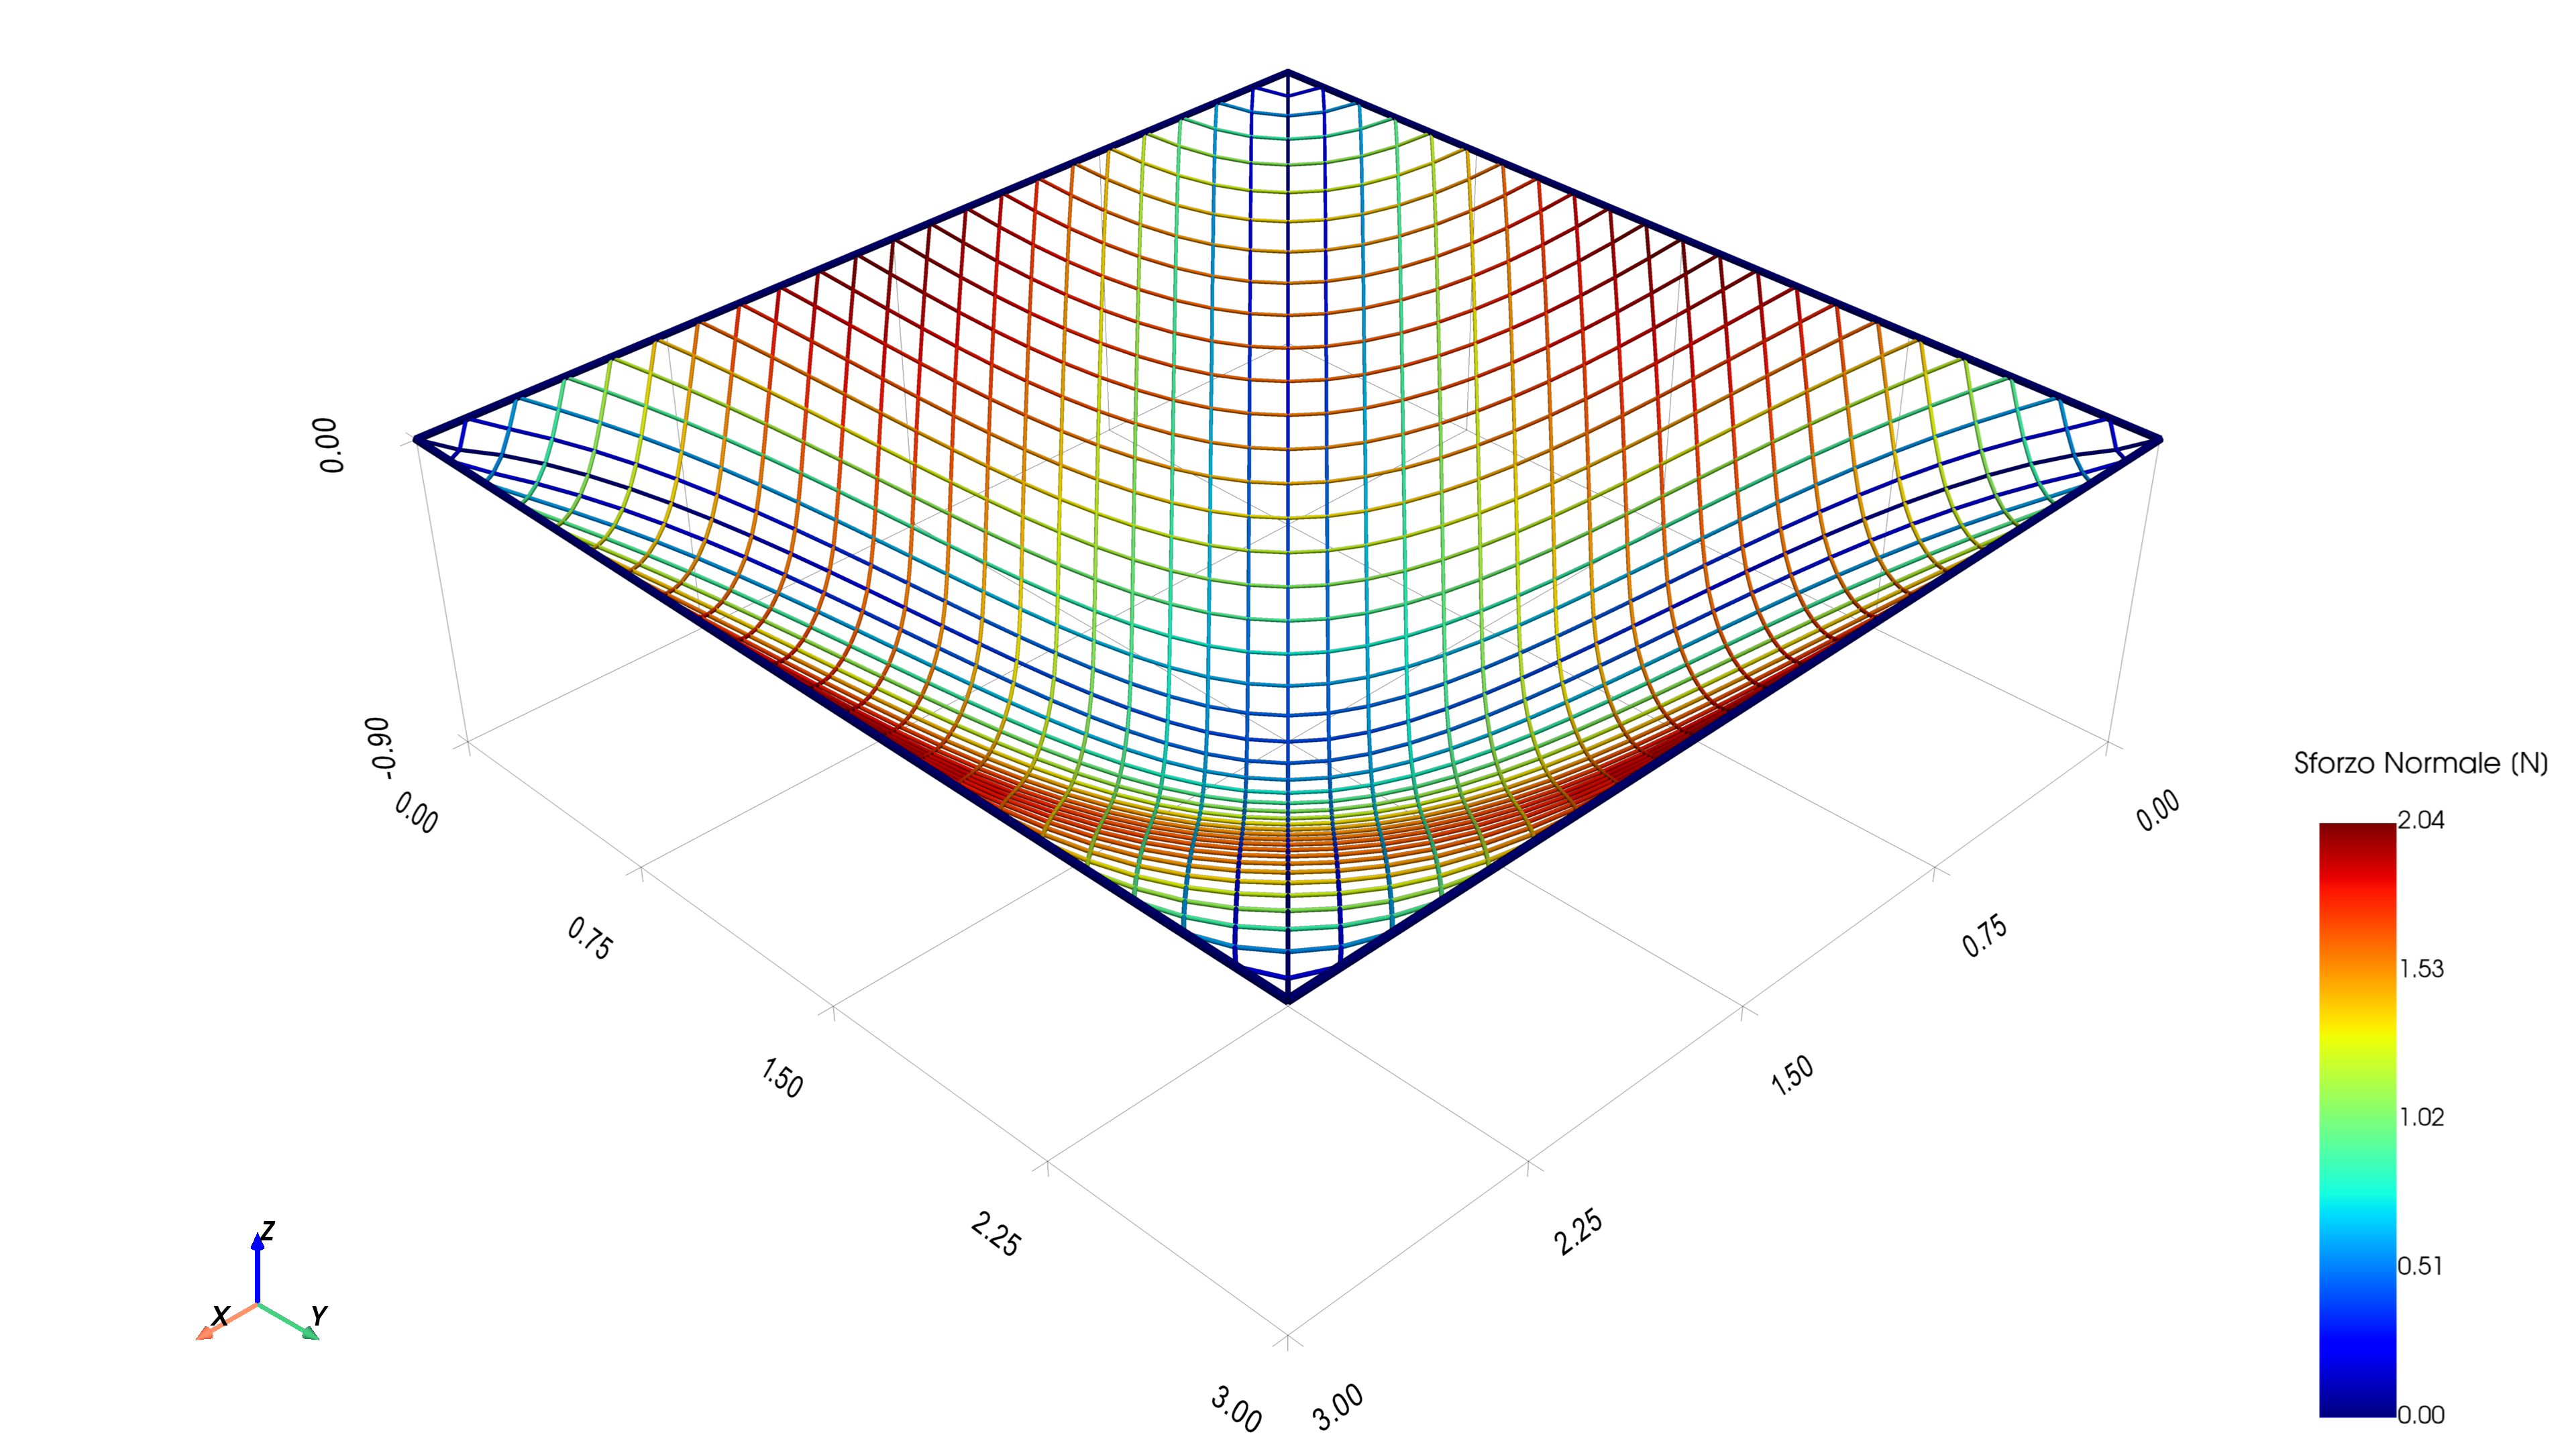
\includegraphics[width=\textwidth]{143_capitoli/capitolo2/immagini_capitolo_2/immagini_slack/rete_D_slack.png}
    \caption{Rete a maglia romboidale in condizione di slack}
    \label{fig:rete_D_slack}
\end{figure}

Questo comportamento discreto trova un parallelo continuo nel campo delle membrane e delle piastre sottili, dove l'insorgere della compressione diagonale provoca un instabilità flessionale fuori dal piano che si manifesta con la formazione di "rughe" parallele alla direzione di trazione principale. In entrambe i sistemi, la struttura modifica la propria topologia tridimensionale attraverso spostamenti fuori dal piano al fine di annullare la compressione interna e minimizzare l'energia potenziale totale del sistema.

Dal punto di vista numerico, l'insorgere dello \textit{slack} comporta l'annullamento delle rigidezza di ampie porzioni della rete. Quando lo sforzo normale nei cavi si annulla la matrice di rigidezza tangente globale del sistema diventa singolare. Fisicamente, ciò corrisponde alla formazione di veri e propri cinematismi locali che rendono il sistema statico indeterminato, ammettendo infinite soluzioni cinematicamente ammissibili. Per superare questa limitazione computazionale e restituire unicità alla soluzione numerica, si ricorre principalmente a due approcci: 

\begin{itemize}
   \item Analisi dinamica: invece di risolvere il problema statico di un sistema labile, si formula un problema dinamico introducendo le forze d'inerzia ed uno smorzamento. L'equazione del moto assume la forma vista in \cref{eq:equilibrio_dinamico_problema}, dove $\underline{p}$ in tal caso è sostituito dal vettore globale delle forze peso definito in \cref{eq:vettore_peso}. Il sistema viene lasciato oscillare sotto l'azione del peso proprio fino a quando lo smorzamento non dissipa l'energia cinetica, conducendo la rete ad una configurazione di equilibrio statico finale, aggirando la singolarità della matrice di rigidezza.
   \item Regolarizzazione della legge costitutiva: uno stratagemma numerico utilizzato nei codici di calcolo consiste nell'evitare che tensione e modulo elastico dell'elemento fune siano nulli. Si introduce una legge costitutiva modificata per la quale quando il cavo subisce un accorciamento, lo sforzo di trazione ed il modulo elastico non scendono a zero ma si stabilizzano su valori infinitesimi positivi (nel nostro caso si è assunto $\sigma \approx 1Pa$ e $E_{eff} \approx 1e^{-2}Pa$). Questa minima rigidezza residua impedisce alla matrice globale di diventare singolare, garantendo la convergenza dell'algoritmo di Newton-Raphson e preservando l'aderenza fisica del modello, in quanto lo sforzo residuo calcolato risulta strutturalmente trascurabile.
\end{itemize}

\subsubsection{Regolarizzazione del legame costitutivo}
Come analizzato in precedenza, il modello costitutivo ideale per un elemento fune in campo elastico, a causa della sua incapacità di sopportare sforzi di compressione, è il modello unilatero denominato \textit{tension-only}. Nella formulazione riportata in \cref{eq:tension_only2}, tale comportamento viene descritto da una funzione bilineare a tratti.

Tuttavia, l'utilizzo di una funzione a tratti presenta un punto in corrispindenza dell'origine in cui la funzione non risulta derivabile. Gli algoritmi di risoluzione come il metodo di Newton-Raphson, mostrano difficoltà di convergenza in presenza di relazioni costitutive non derivabili, a causa delle brusche oscillazioni della rigidezza tangente nei punti di transizione. 

Per superare tale limitazione computazionale e favorire la convergenza numerica nel calcolo delle reti lasche si è adottata la regolarizzazione della legge costitutiva. Nello specifico, la relazione bilineare viene approssimata tramite una funzione derivabile su tutto il suo dominio $(e_{11} \in [-\infty, \infty])$. La relazione costitutiva regolarizzata assume pertanto la forma:
\begin{equation}
   \sigma = \sigma_{min} + \frac{E}{\beta} \ln\left( 1 + e^{\beta e_{11}} \right) 
   \label{eq:bilinear_smooth}
\end{equation}

dove: 
\begin{itemize}
   \item $E$ rappresenta il modulo elastico del materiale nel tratto teso;
   \item $e_{11}$ è la componente assiale del tensore di deformazione di Green-Lagrange;
   \item $\sigma_{min}$ è il valore di tensione minima residua;
   \item $\beta$ è un parametro di regolarizzazione adimensionale che governa la transizione tra il comportamento lasco e quello teso.
\end{itemize}

La scelta del parametro $\beta$ rappresenta un compromesso di fondamentale importanza: l'impiego di valori di $\beta$ elevati consentono di approssimare con estrema fedeltà la legge bilineare ideale, ma introducono gradienti che penalizzano la stabilità dell'algoritmo di soluzione. Al contrario, valori di $\beta$ contenuti migliorano significativamente la convergenza a discapito, però, della rispondenza fisica del modello nell'intorno del punto in cui $e_{11} \approx 0$.

Come mostrato in (mettiamo il riferimento del grafico con i due legami costitutivi smooth e bilineare puro), la formulazione regolarizzata descritta dall'\cref{eq:bilinear_smooth} riprende fedelmente l'andamento della legge \textit{tension-only} classica, garantendo al contempo la continuità della derivata prima su tutto il dominio di definizione. 

\begin{figure}[H]
   \centering
    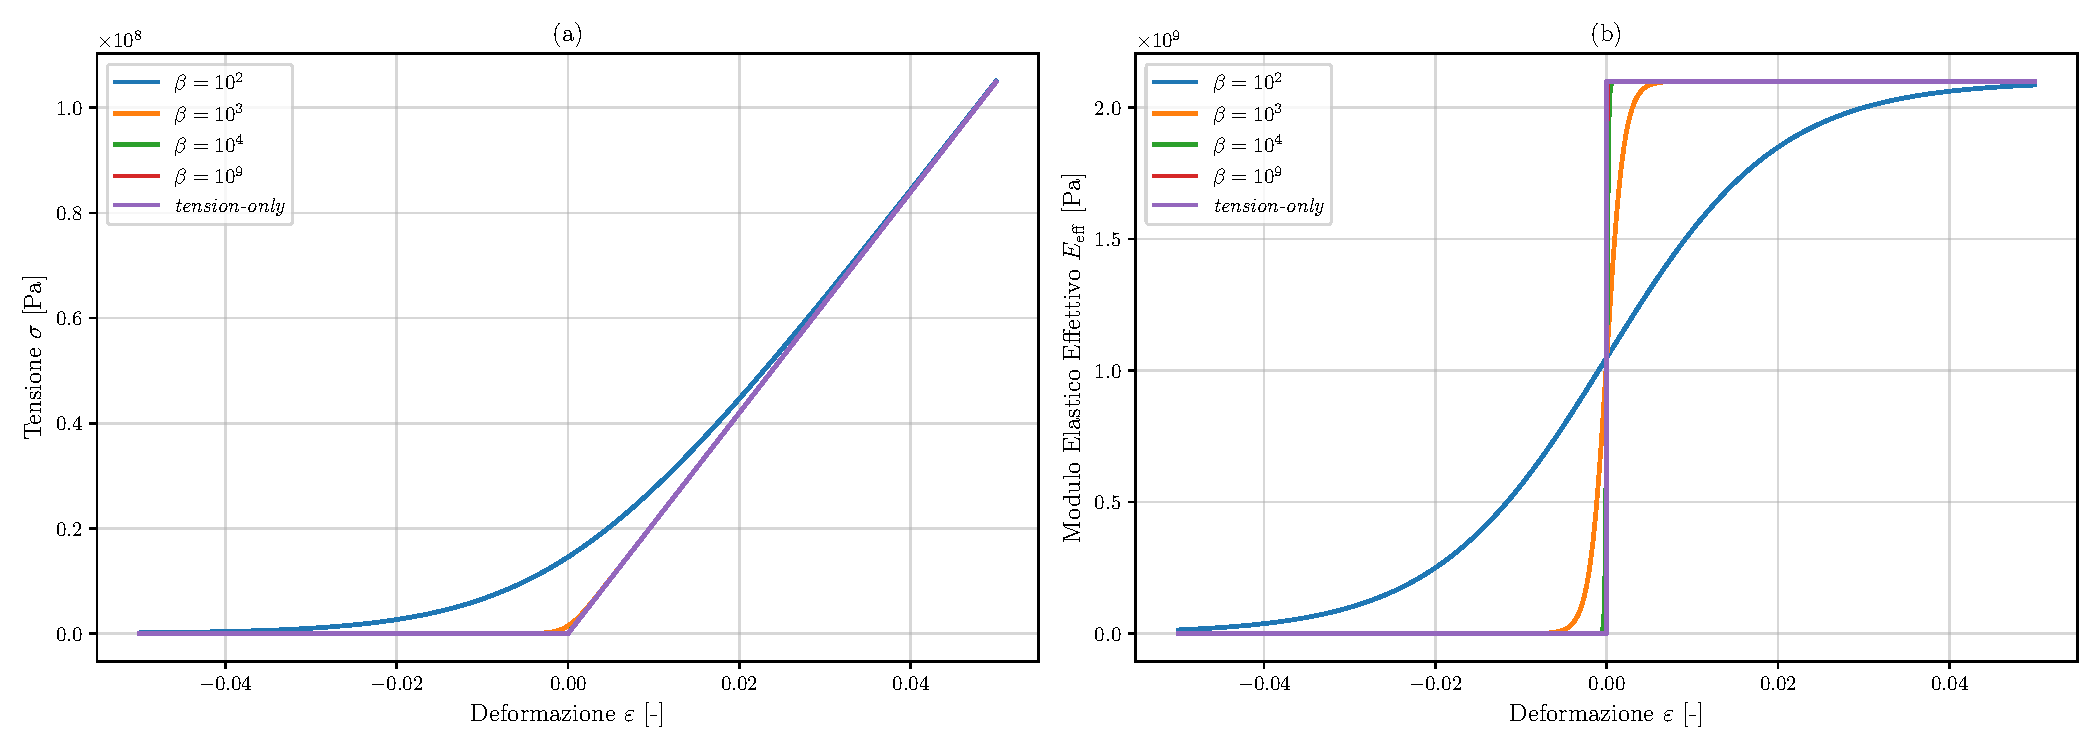
\includegraphics[width=\textwidth]{143_capitoli/capitolo2/immagini_capitolo_2/immagini_slack/Legame_regolarizzato2.pdf}
    \caption{(a) Legame Costitutivo Regolarizzato $\sigma - \varepsilon$ -  (b) Modulo Elastico $E_{\mathrm{eff}} - \varepsilon$}
    \label{fig:legame_costitutivo_regolarizzato}
\end{figure}

\subsubsection{Laschezza della rete}
La valutazione della freccia massima (\textit{sag}) al variare dello sviluppo lineare della rete rispetto alla distanza tra i vincoli può essere espressa quantitativamente attraverso un parametro adimensionale che prende il nome di \textit{rapporto di laschezza} o \textit{slackness ratio}.

Al fine di stimare l'entità della freccia iniziale della rete e garantire il rispetto delle prescrizioni geometriche imposte dalla normativa \cite{EN1263-1} per la prova statica di assorbimento di energia della rete, si è condotta un analisi parametrica su una rete di dimensioni nominali pari a $3\, \text{m} \times 3\,\text{m}$ (come previsto dalla norma circa la stessa prova), ipotizzando un medesimo valore di \textit{rapporto di laschezza} lungo entrambe le direzioni principali. Nello specifico, è stata determinata la curva caratteristica che correla il rapporto di laschezza al valore della freccia massima risultante.

I risultati di tale analisi, relativi sia alla configurazione con rete a maglia quadrata (Q) sia a quella con maglia a geometria romboidale (D), sono illustrati rispettivamente in \cref{fig:diagramma_sag_Q} e in \cref{fig:diagramma_sag_D}. Dall'esame degli andamenti dei grafici si evince che la tolleranza sulla lunghezza dei lati della rete quadrata in esame dovrà essere confinata entro i limiti individuati per le due differenti geometrie, al fine di scongiurare un eccessiva deformabilità o, al contrario, uno stato di coazione iniziale indesiderato.

\begin{figure}[H]
   \centering
    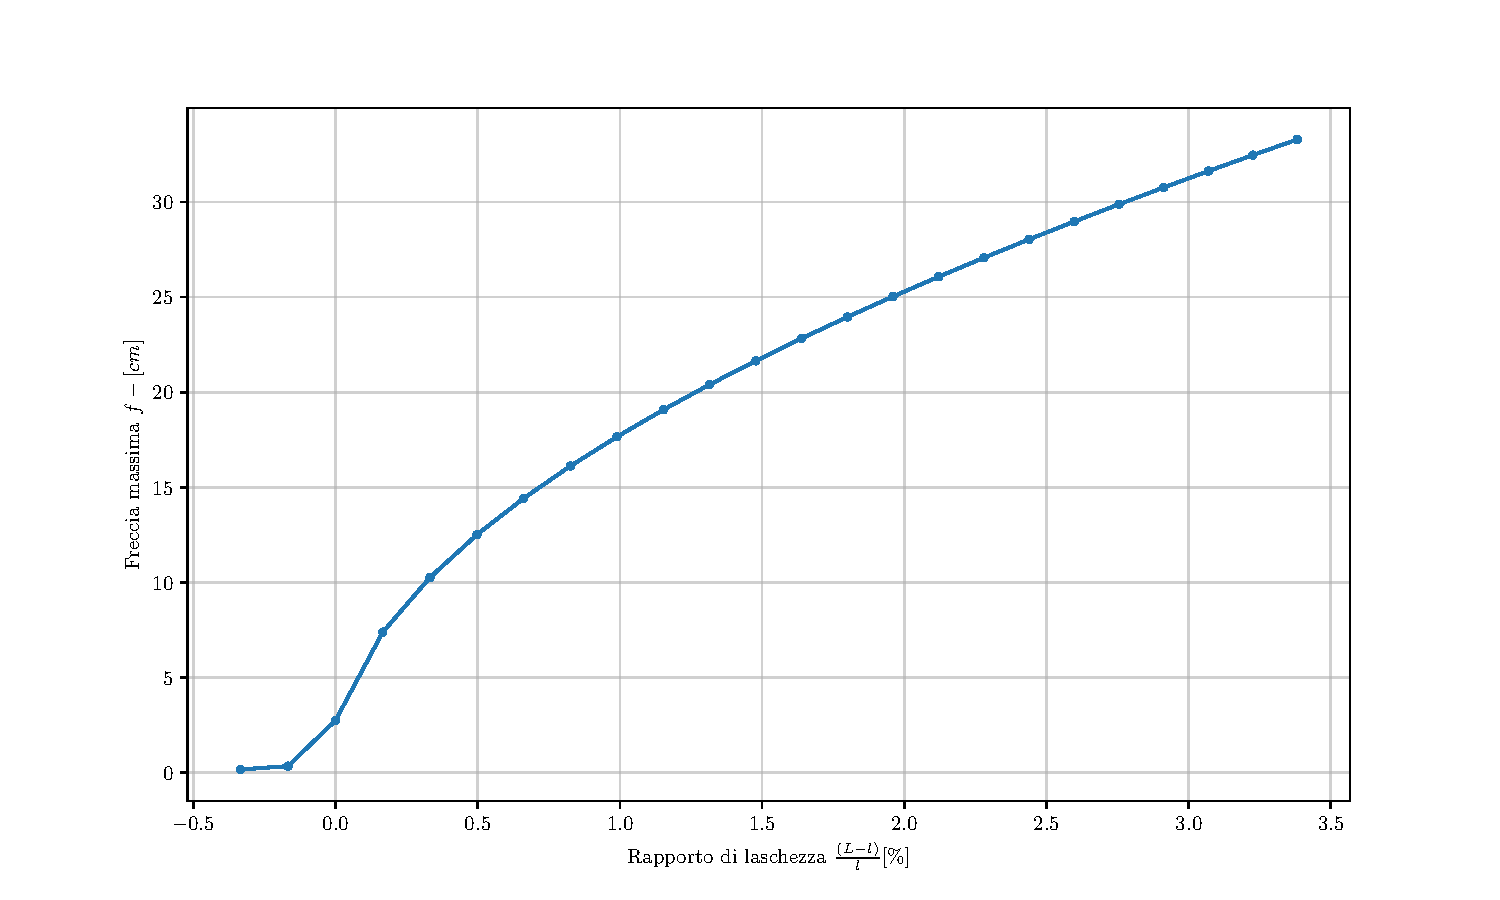
\includegraphics[width=\textwidth]{143_capitoli/capitolo2/immagini_capitolo_2/immagini_slack/grafico_Q.pdf}
    \caption{Diagramma \textit{sag} - \textit{slackness ratio} per una rete a maglia quadrata}
    \label{fig:diagramma_sag_Q}
\end{figure}

\begin{figure}[H]
   \centering
    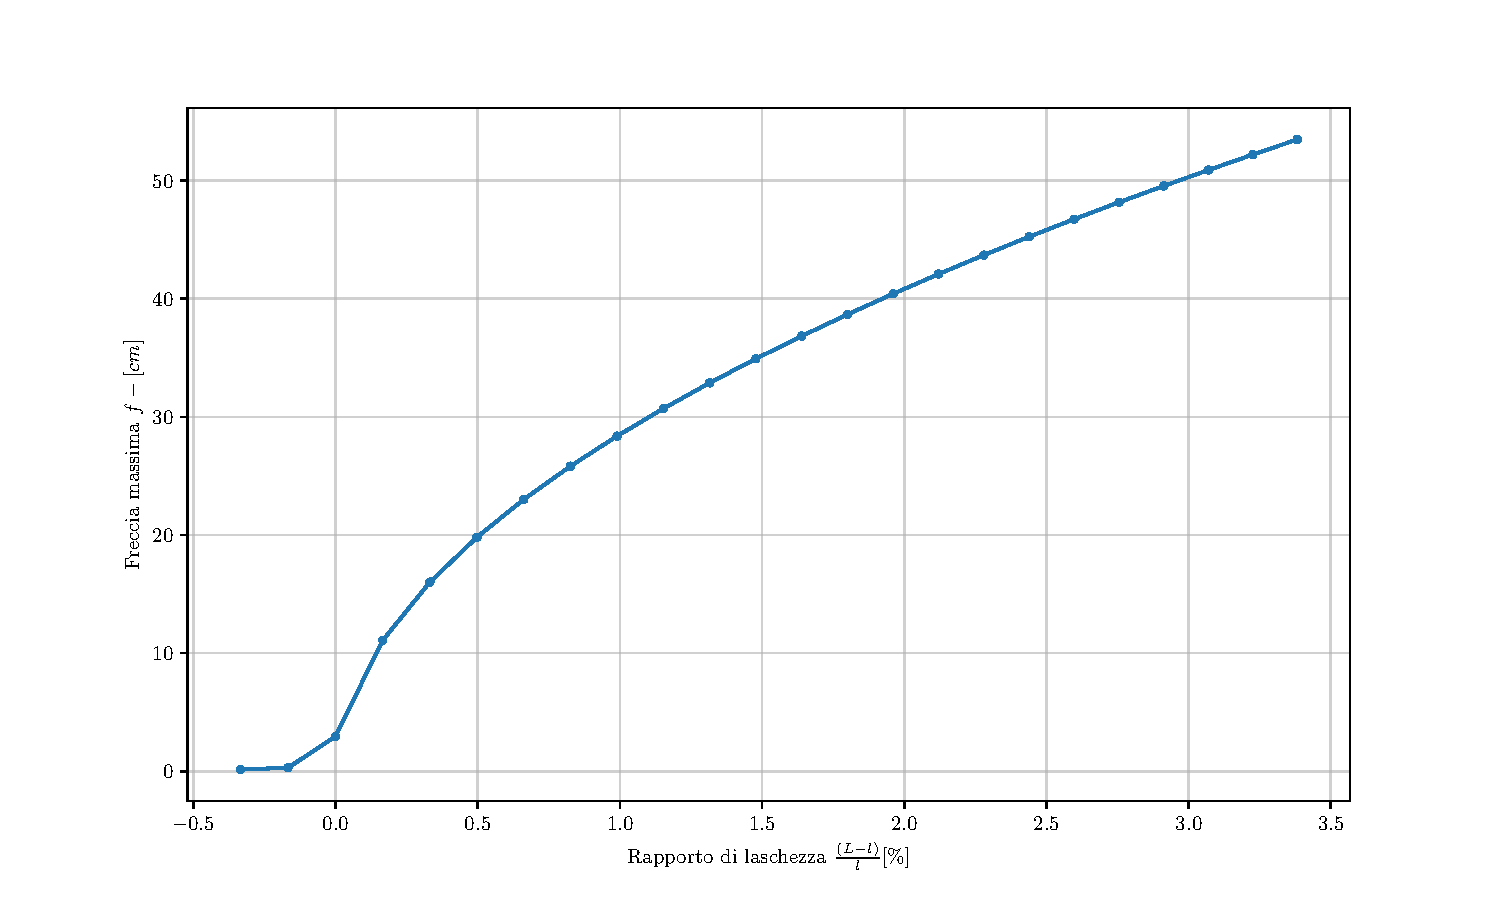
\includegraphics[width=\textwidth]{143_capitoli/capitolo2/immagini_capitolo_2/immagini_slack/grafico_D.pdf}
    \caption{Diagramma \textit{sag} - \textit{slackness ratio} per una rete a maglia romboidale}
    \label{fig:diagramma_sag_D}
\end{figure}

\subsection{Carichi concentrati}
Fino ad ora l'analisi numerica si è concentrata esclusivamente sulla configurazione di equilibrio della rete soggetta al solo peso proprio; nello specifico, nell'\cref{eq:problema_statico} si è assunto che il vettore dei carichi esterni fosse pari a: 
\begin{equation}
   \underline{f}_{ext} = \underline{f}_{g,e}
\end{equation}

Tuttavia, l'algoritmo implementato consente di estendere la trattazione includendo l'applicazione di forze concentrate, caratterizzate da intensità e direzioni arbitrarie, agenti su nodi specifici della mesh. In questo scenario, l'espressione del vettore dei carichi esterni si specifica per mezzo della relazione:
\begin{equation}
   \underline{f}_{ext} = \underline{f}_{g,e} + \underline{f}_{concentrate} 
\end{equation}

Ulteriori sviluppi e applicazioni del codice potranno prevedere l'implementazione di combinazioni lineari di vettori di forze concentrate. Tale approccio consentirà di simulare, in forma discretizzata, distribuizioni di carico continue in funzione delle esigenze dell'utente.

A scopo dimostrativo, in (metto riferimento della figura con rete soggetta a fune concentrata), viene illustrata la configurazione deformata e lo stato tensionale della rete ottenuti applicando una forza concentrata in corrispondenza del nodo di mezzeria. 
